\documentclass[10pt,]{scrartcl}
\usepackage{lmodern}
\usepackage{amssymb,amsmath}
\usepackage{ifxetex,ifluatex}
\usepackage{fixltx2e} % provides \textsubscript
\ifnum 0\ifxetex 1\fi\ifluatex 1\fi=0 % if pdftex
  \usepackage[T1]{fontenc}
  \usepackage[utf8]{inputenc}
\else % if luatex or xelatex
  \ifxetex
    \usepackage{mathspec}
  \else
    \usepackage{fontspec}
  \fi
  \defaultfontfeatures{Ligatures=TeX,Scale=MatchLowercase}
\fi
% use upquote if available, for straight quotes in verbatim environments
\IfFileExists{upquote.sty}{\usepackage{upquote}}{}
% use microtype if available
\IfFileExists{microtype.sty}{%
\usepackage[]{microtype}
\UseMicrotypeSet[protrusion]{basicmath} % disable protrusion for tt fonts
}{}
\PassOptionsToPackage{hyphens}{url} % url is loaded by hyperref
\usepackage[unicode=true]{hyperref}
\PassOptionsToPackage{usenames,dvipsnames}{color} % color is loaded by hyperref
\hypersetup{
            pdftitle={Personal attacks decrease user activity in social networking platforms},
            pdfauthor={Rafal Urbaniak (LoPSE research group, University of Gdansk); Michał Ptaszyński (Kitami Institute of Technology); Patrycja Tempska, Gniewosz Leliwa, Maciej Brochocki, Michał Wroczyński (Samurai Labs)},
            colorlinks=true,
            linkcolor=Maroon,
            citecolor=Blue,
            urlcolor=blue,
            breaklinks=true}
\urlstyle{same}  % don't use monospace font for urls
\usepackage{color}
\usepackage{fancyvrb}
\newcommand{\VerbBar}{|}
\newcommand{\VERB}{\Verb[commandchars=\\\{\}]}
\DefineVerbatimEnvironment{Highlighting}{Verbatim}{commandchars=\\\{\}}
% Add ',fontsize=\small' for more characters per line
\usepackage{framed}
\definecolor{shadecolor}{RGB}{248,248,248}
\newenvironment{Shaded}{\begin{snugshade}}{\end{snugshade}}
\newcommand{\KeywordTok}[1]{\textcolor[rgb]{0.13,0.29,0.53}{\textbf{#1}}}
\newcommand{\DataTypeTok}[1]{\textcolor[rgb]{0.13,0.29,0.53}{#1}}
\newcommand{\DecValTok}[1]{\textcolor[rgb]{0.00,0.00,0.81}{#1}}
\newcommand{\BaseNTok}[1]{\textcolor[rgb]{0.00,0.00,0.81}{#1}}
\newcommand{\FloatTok}[1]{\textcolor[rgb]{0.00,0.00,0.81}{#1}}
\newcommand{\ConstantTok}[1]{\textcolor[rgb]{0.00,0.00,0.00}{#1}}
\newcommand{\CharTok}[1]{\textcolor[rgb]{0.31,0.60,0.02}{#1}}
\newcommand{\SpecialCharTok}[1]{\textcolor[rgb]{0.00,0.00,0.00}{#1}}
\newcommand{\StringTok}[1]{\textcolor[rgb]{0.31,0.60,0.02}{#1}}
\newcommand{\VerbatimStringTok}[1]{\textcolor[rgb]{0.31,0.60,0.02}{#1}}
\newcommand{\SpecialStringTok}[1]{\textcolor[rgb]{0.31,0.60,0.02}{#1}}
\newcommand{\ImportTok}[1]{#1}
\newcommand{\CommentTok}[1]{\textcolor[rgb]{0.56,0.35,0.01}{\textit{#1}}}
\newcommand{\DocumentationTok}[1]{\textcolor[rgb]{0.56,0.35,0.01}{\textbf{\textit{#1}}}}
\newcommand{\AnnotationTok}[1]{\textcolor[rgb]{0.56,0.35,0.01}{\textbf{\textit{#1}}}}
\newcommand{\CommentVarTok}[1]{\textcolor[rgb]{0.56,0.35,0.01}{\textbf{\textit{#1}}}}
\newcommand{\OtherTok}[1]{\textcolor[rgb]{0.56,0.35,0.01}{#1}}
\newcommand{\FunctionTok}[1]{\textcolor[rgb]{0.00,0.00,0.00}{#1}}
\newcommand{\VariableTok}[1]{\textcolor[rgb]{0.00,0.00,0.00}{#1}}
\newcommand{\ControlFlowTok}[1]{\textcolor[rgb]{0.13,0.29,0.53}{\textbf{#1}}}
\newcommand{\OperatorTok}[1]{\textcolor[rgb]{0.81,0.36,0.00}{\textbf{#1}}}
\newcommand{\BuiltInTok}[1]{#1}
\newcommand{\ExtensionTok}[1]{#1}
\newcommand{\PreprocessorTok}[1]{\textcolor[rgb]{0.56,0.35,0.01}{\textit{#1}}}
\newcommand{\AttributeTok}[1]{\textcolor[rgb]{0.77,0.63,0.00}{#1}}
\newcommand{\RegionMarkerTok}[1]{#1}
\newcommand{\InformationTok}[1]{\textcolor[rgb]{0.56,0.35,0.01}{\textbf{\textit{#1}}}}
\newcommand{\WarningTok}[1]{\textcolor[rgb]{0.56,0.35,0.01}{\textbf{\textit{#1}}}}
\newcommand{\AlertTok}[1]{\textcolor[rgb]{0.94,0.16,0.16}{#1}}
\newcommand{\ErrorTok}[1]{\textcolor[rgb]{0.64,0.00,0.00}{\textbf{#1}}}
\newcommand{\NormalTok}[1]{#1}
\usepackage{graphicx,grffile}
\makeatletter
\def\maxwidth{\ifdim\Gin@nat@width>\linewidth\linewidth\else\Gin@nat@width\fi}
\def\maxheight{\ifdim\Gin@nat@height>\textheight\textheight\else\Gin@nat@height\fi}
\makeatother
% Scale images if necessary, so that they will not overflow the page
% margins by default, and it is still possible to overwrite the defaults
% using explicit options in \includegraphics[width, height, ...]{}
\setkeys{Gin}{width=\maxwidth,height=\maxheight,keepaspectratio}
\IfFileExists{parskip.sty}{%
\usepackage{parskip}
}{% else
\setlength{\parindent}{0pt}
\setlength{\parskip}{6pt plus 2pt minus 1pt}
}
\setlength{\emergencystretch}{3em}  % prevent overfull lines
\providecommand{\tightlist}{%
  \setlength{\itemsep}{0pt}\setlength{\parskip}{0pt}}
\setcounter{secnumdepth}{5}
% Redefines (sub)paragraphs to behave more like sections
\ifx\paragraph\undefined\else
\let\oldparagraph\paragraph
\renewcommand{\paragraph}[1]{\oldparagraph{#1}\mbox{}}
\fi
\ifx\subparagraph\undefined\else
\let\oldsubparagraph\subparagraph
\renewcommand{\subparagraph}[1]{\oldsubparagraph{#1}\mbox{}}
\fi

% set default figure placement to htbp
\makeatletter
\def\fps@figure{htbp}
\makeatother

%\documentclass{article}

% %packages
 \usepackage{booktabs}
 \usepackage[sort&compress]{natbib}
\usepackage{graphicx}
\usepackage{longtable}
\usepackage{ragged2e}
\usepackage{etex}
%\usepackage{yfonts}
\usepackage{marvosym}
\usepackage[notextcomp]{kpfonts}
\usepackage{nicefrac}
\newcommand*{\QED}{\hfill \footnotesize {\sc Q.e.d.}}
\usepackage{multicol} 
%\usepackage[textsize=footnotesize]{todonotes}
%\linespread{1.5}

\usepackage{xcolor}

\setlength{\parindent}{10pt}
\setlength{\parskip}{1pt}


%language
%\usepackage{times}
\usepackage{mathptmx}
\usepackage[scaled=0.88]{helvet}

\usepackage{t1enc}
%\usepackage[utf8x]{inputenc}
%\usepackage[polish]{babel}
%\usepackage{polski}

\usepackage{subcaption}


%AMS
\usepackage{amsfonts}
\usepackage{amssymb}
\usepackage{amsthm}
\usepackage{amsmath}

%\usepackage{geometry}
 %\geometry{a4paper,left=35mm,top=20mm,}

%abbreviations
\newcommand{\ra}{\rangle}
\newcommand{\la}{\langle}
\newcommand{\n}{\neg}
\newcommand{\et}{\wedge}
\newcommand{\jt}{\rightarrow}
\newcommand{\ko}[1]{\forall  #1\,}
\newcommand{\ro}{\leftrightarrow}
\newcommand{\exi}[1]{\exists\, {_{#1}}}
\newcommand{\pr}{\mathsf{P}}
\newcommand{\odds}{\mathsf{Odds}}
\newcommand{\ind}{\mathsf{Ind}}
\newcommand{\nf}[2]{\nicefrac{#1\,}{#2}}
\newcommand{\R}[1]{\texttt{#1}}

\newtheorem{q}{\color{blue}Question}


%% Rafal's stuff
\usepackage[margin=1.5in,top=1in]{geometry}
\usepackage[textsize=scriptsize, textwidth = 3cm]{todonotes}
% This is my own comment shading, keep \todo for general stuff, feel free to define your own separate comment colors (usually useful if you use margin comments at tall) For instance, I defined one for Patrycja
\newcommand{\rt}[1]{\todo[color = orange!40]{#1}}
\newcommand{\pt}[1]{\todo[color = blue!40]{#1}}




\newtheorem*{reply*}{Reply}
\usepackage{enumitem}
\newcommand{\question}[1]{\begin{enumerate}[resume,leftmargin=0cm,labelsep=0cm,align=left]
\item #1
\end{enumerate}}

\usepackage{float}

% \setbeamertemplate{blocks}[rounded][shadow=true]
% \setbeamertemplate{itemize items}[ball]
% \AtBeginPart{}
% \AtBeginSection{}
% \AtBeginSubsection{}
% \AtBeginSubsubsection{}
% \setlength{\emergencystretch}{0em}
% \setlength{\parskip}{0pt}
\usepackage{booktabs}
\usepackage{longtable}
\usepackage{array}
\usepackage{multirow}
\usepackage{wrapfig}
\usepackage{float}
\usepackage{colortbl}
\usepackage{pdflscape}
\usepackage{tabu}
\usepackage{threeparttable}
\usepackage{threeparttablex}
\usepackage[normalem]{ulem}
\usepackage{makecell}
\usepackage{xcolor}

\title{Personal attacks decrease user activity in social networking platforms}
\author{\normalsize Rafal Urbaniak
(\href{http://lopsegdansk.blogspot.com/p/lopse-team.html}{LoPSE research
group}, University of Gdansk) \and \normalsize Michał Ptaszyński (Kitami Institute of Technology) \and \normalsize Patrycja Tempska, Gniewosz Leliwa, Maciej Brochocki, Michał
Wroczyński (Samurai Labs)}
\date{}

\begin{document}
\maketitle

\vspace{-2mm}

\begin{abstract}
\noindent \textbf{Abstract.} 
We conduct a large scale data-driven analysis of the effects of online personal attacks on social media user activity. First, we perform a thorough overview of the literature on the influence of social media on user behavior, especially on the impact that negative and aggressive behaviors, such as harassment and cyberbullying, have on users’ engagement in online media platforms. The majority of previous research were  small-scale self-reported studies, which is their limitation. This motivates our data-driven study. We perform a large-scale analysis of messages from Reddit, a discussion website, for a period of two weeks, involving 182,528 posts or comments to posts by 148,317 users. To efficiently collect and analyze the data we apply a high-precision personal attack detection technology. We analyze the obtained data from three perspectives: (i) classical statistical methods, (ii) Bayesian estimation, and (iii) model-theoretic analysis. The three perspectives agree: personal attacks decrease the victims’ activity.
The results can be interpreted as an important signal to social media platforms and policy makers that leaving personal attacks unmoderated is quite likely to disengage the users and in effect depopulate the platform. On the other hand, application of cyberviolence detection technology in combination with various mitigation techniques could improve and strengthen the user community. As more of our lives is taking place online, keeping the virtual space inclusive for all users becomes an important problem which online media platforms need to face.
\end{abstract}

\vspace{2cm}

\textbf{Remark.} In what follows, we sometimes display key pieces of
code and explain what it does. Some not too fascinating pieces of code
are supressed, but the reader can look them up in the associated .Rmd
file and compile their own version.

\section{Technology applied for personal attack detection}
\label{technology}

For the need of this research we define \textit{personal attack} as any
kind of abusive remark made in relation to a person
(\textit{ad hominem}) rather than to the content of the argument
expressed by that person in a discussion. The definition of `personal
attack' subsumes the use of specific terms which compare other people to
animals or objects or making nasty insinuations without providing
evidence. Three examples of typical personal attacks are as follows.

\begin{itemize} 
\item \emph{You are legit mentally retarded homie.}
\item \emph {Eat a bag of dicks, fuckstick.}
\item \emph {Fuck off with your sensitivity you douche.} 
\end{itemize}

The detection of personal attacks was performed using Samurai, a
proprietary technology of Samurai Labs.\footnote{\url{https://www.samurailabs.ai/},
  described in (Ptaszyński, Leliwa, Piech, \& Smywiński-Pohl, 2018;
  Wroczynski \& Leliwa, 2019).} The technology comprises a combination
of symbolic and statistical methods, where each statistical component
(e.g., a deep learning model) is governed by a symbolic component
utilizing a variety of natural language processing methods (e.g.,
tokenization, syntactic parsing, etc.). Symbolic components are used to
determine if a potentially abusive utterance is not a part of a broader
utterance indicating that the first one should not be considered
abusive. For example, an utterance ``you are an idiot'' is potentially
abusive, but it really is not, if it appears as a part of some broader
utterance such as ``I cannot believe he said you are an idiot.'' Another
example of using symbolic components is determining if an abusive phrase
is targeted against an interlocutor (e.g.~using a linking verb to assign
the abusive phrase with a second person as in the ``you are an idiot''
example).

Samurai (Wroczynski \& Leliwa, 2019) employs a compositional approach,
where each problem is divided into a set of corresponding sub-problems
represented with language phenomena (e.g., speech acts), and detected
independently using highly precise contextual models. For example,
personal attacks comprise a high-level category that can be divided into
language phenomena (mid-level categories) such as insulting (using
abusive terms in relation to other people), comparing other people to
animals (e.g., ``looks like a pig'') or objects (e.g., ``smells like an
old sock''), or making insinuating remarks (e.g., ``I heard she had sex
with her students''). Furthermore, each mid-level category can be
further decomposed into low-level categories. For example, insulting can
be expressed by using a linking verb (e.g., ``you are an idiot'') or a
vocative case (e.g. ``stop talking to me, idiot'').

Figure \ref{fig:samuraiexample} illustrates how the input text (``ccant
believ he sad ur an id10+\ldots{}!'') is processed step-by-step
utilizing both statistical and symbolic methods.

\begin{figure}[h]
    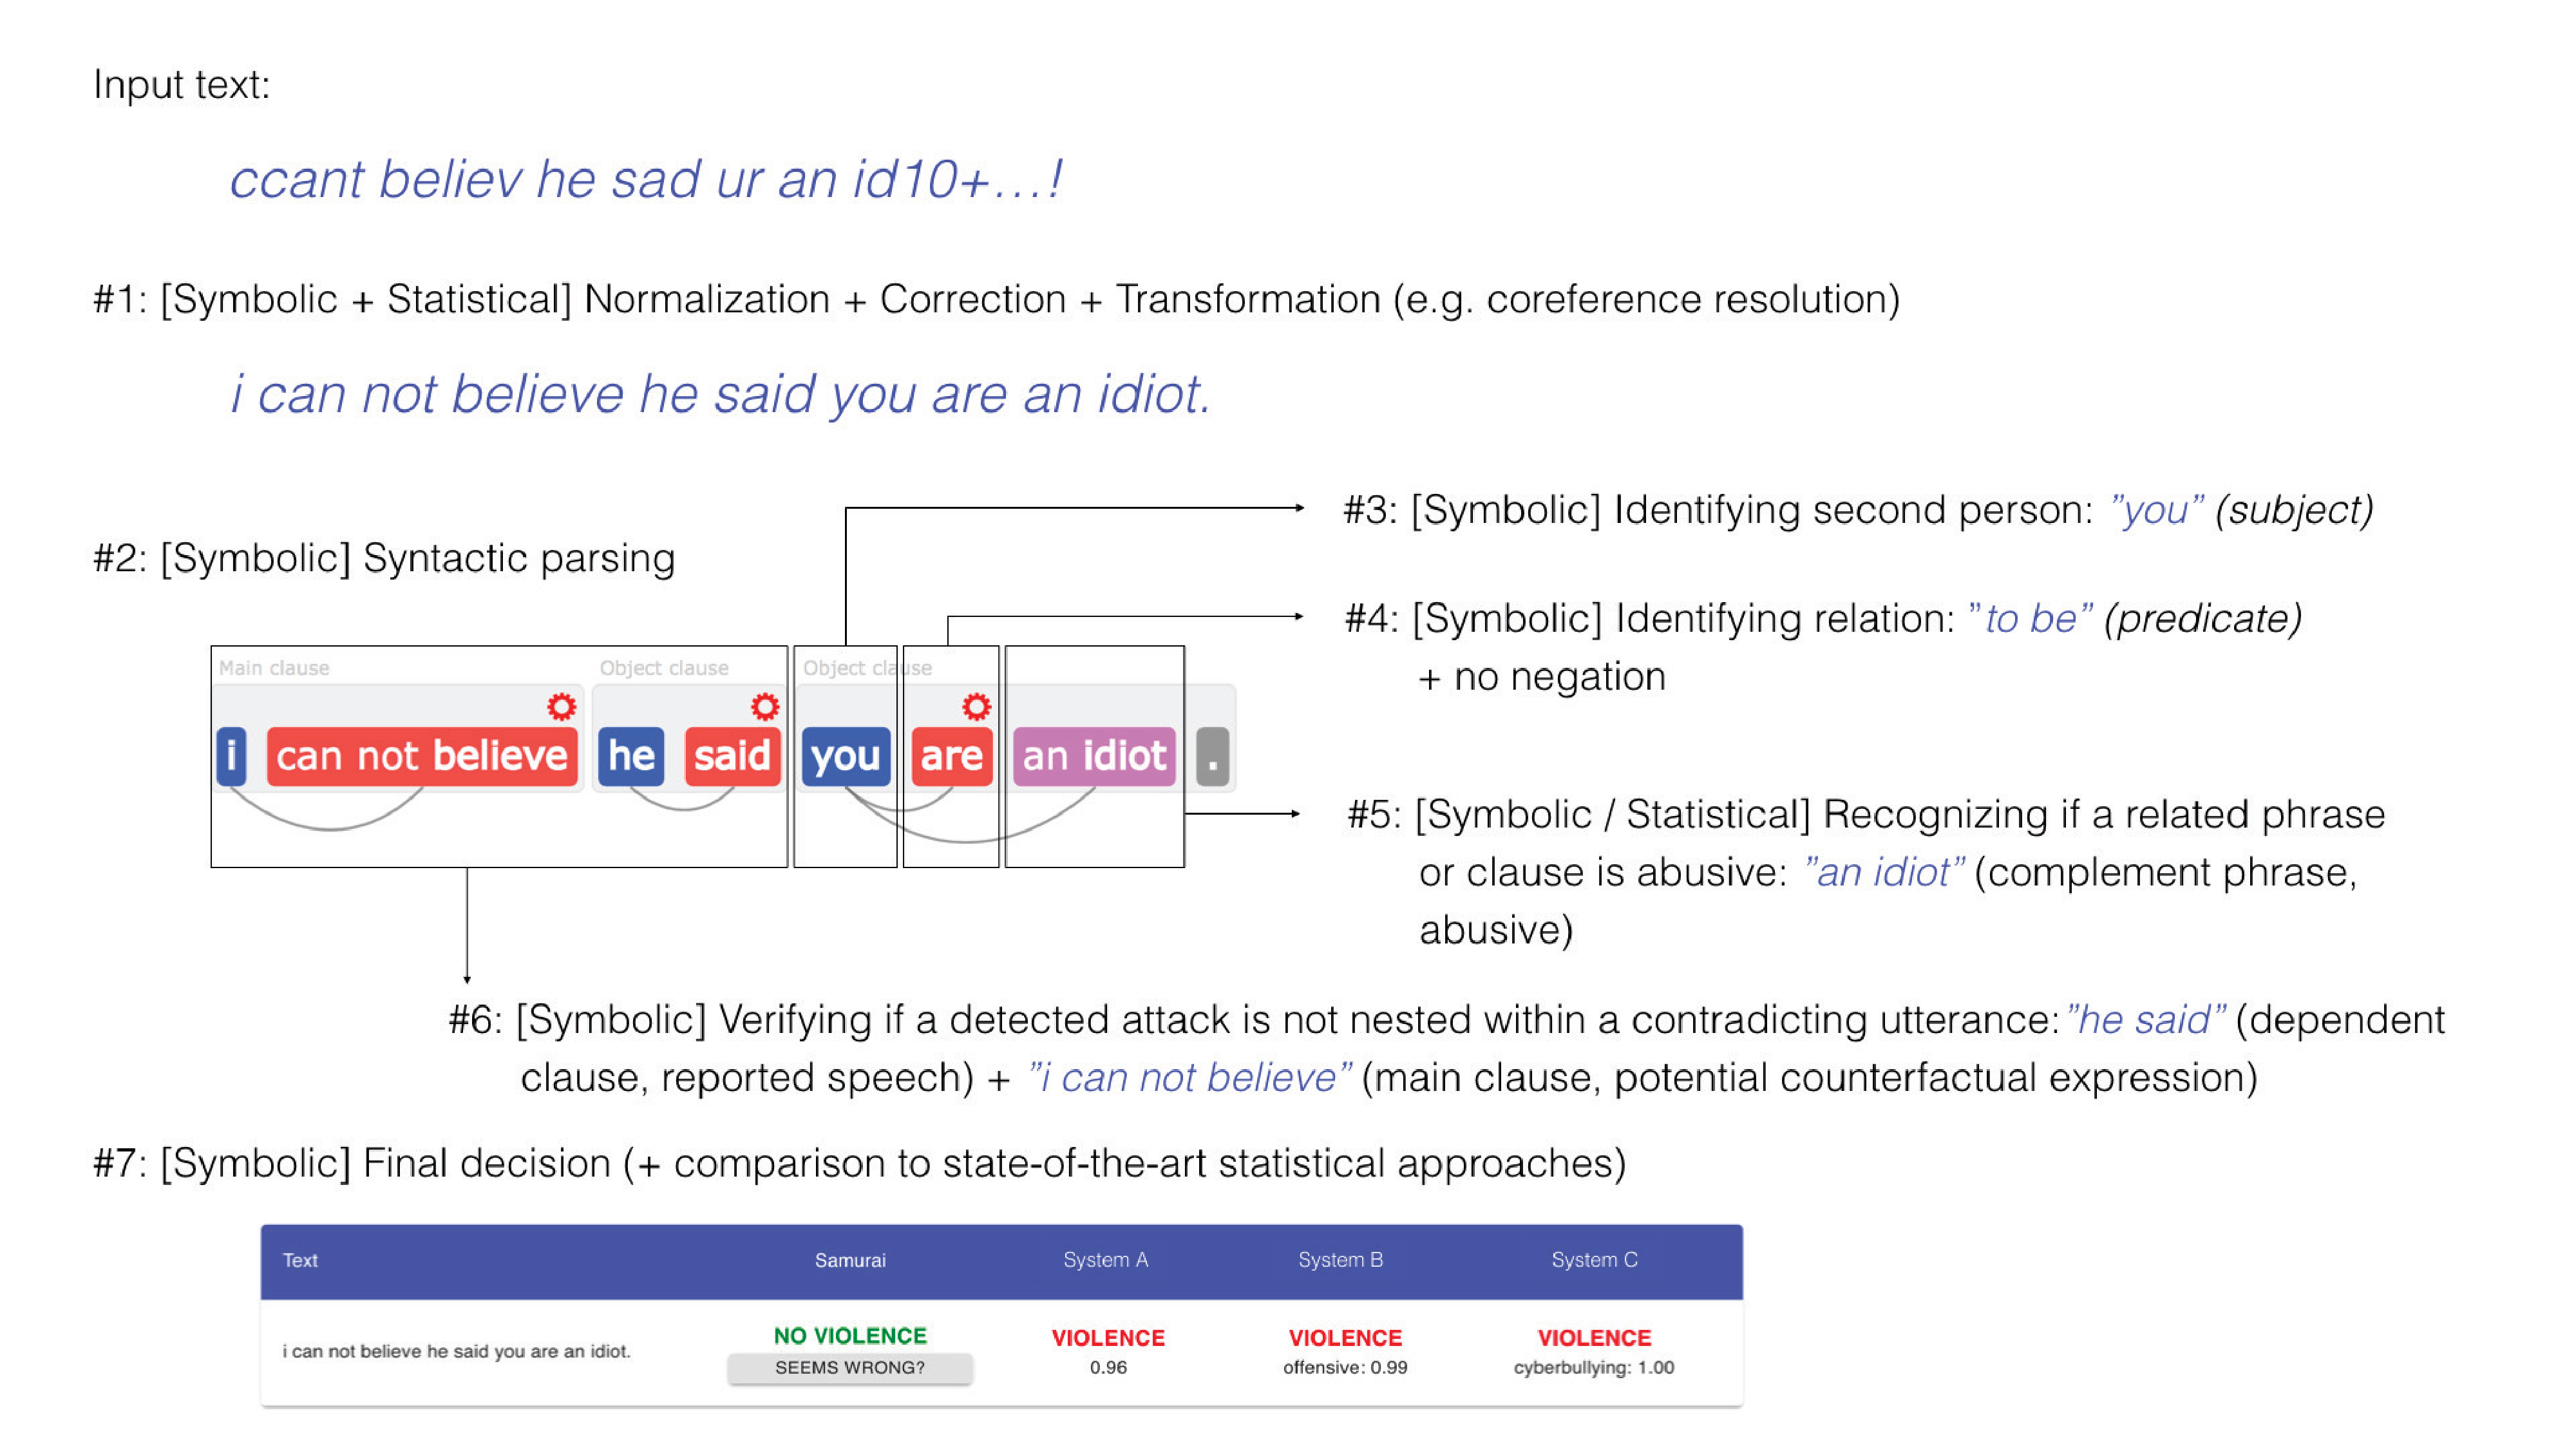
\includegraphics[width=\linewidth]{../images/example-eps-converted-to.pdf}
    \caption{Example of processing of one sentence by the applied Samurai technology.}
    \label{fig:samuraiexample}
\end{figure}

In practice, it means that a whole variety of constructions can be
detected without the need to construct a fixed list of dictionary words
defined \textit{a priori}. Due to utilizing symbolic components that
oversee statistical components, \{\textsf Samurai\} recognizes complex
linguistic phenomena (such as indirect speech, rhetorical figures or
counter-factual expressions) to distinguish personal attacks from normal
communication, greatly reducing the number of false alarms as compared
to others systems used for violence detection. An example of comparison
can be seen in Figure \ref{fig:samuraiexample}, and a full benchmark was
presented in (Ptaszyński et al., 2018).

The detection models utilized in this research were designed to detect
personal attacks targeted against a second person (e.g.~interlocutor,
original author of a post) and a third person/group (e.g., other
participants in the conversation, people not involved in the
conversation, social groups, professional groups), except public figures
(e.g.~politicians, celebrities). With regards to symbolic component of
the system, by ``models'' we mean separate rules (such as, specifying a
candidate for the presence of personal attack, such as the aggressive
word ``idiot,'' which is further disambiguated with a syntactic rule of
citation, e.g., ``{[}he\(\vert\)she\(\vert\)they{]} said {[}SUBJECT{]}
{[}PREDICATE{]}'') or sets of rules, as seen in Figure
\ref{fig:samuraiexample}, e.g.~normalization model contains rules for
transcription normalization, citation detection model contains rules for
citation, etc. With regards to the statistical component, by ``models''
refer to machine learning models trained on large data to classify an
entry into one of the categories (e.g., true personal attack, or false
positive).

Moreover, the symbolic component of the system uses two types of
symbolic rules, namely ``narrow rules'' and ``wide rules.'' The former
have smaller coverage (e.g., are triggered less often), but detect
messages containing personal attacks with high
precision.\footnote{Precision is defined traditionally as the ratio of correctly detected instances among all detected instances.}
The latter, have wider coverage, but their precision is lower. We
decided to set apart the ``narrow'' and ``wide'' subgroups of the
detection models in order to increase the granularity of the analysis.
Firstly, we took only the detection models designed to detect personal
attacks targeted against second person. Secondly, we used these models
on a dataset of 320,000 Reddit comments collected on 2019/05/06.
Thirdly, we randomly picked at most hundred returned results for each
low-level
model\footnote{Low-level models are responsible for detecting low-level categories. Similarly, mid-level models detect mid-level categories, by combining several low-level models, etc.}
(some models are triggered very often while others rarely, so using all
instances would create too much bias). There were 390 low-level models
but many of them returned in less than 100 results. We verified them
manually with the help of expert annotators trained in detection of
personal attacks and selected only those models that achieved at least
90\% of precision. The models with fewer than 100 returned results were
excluded from the selection. After this step, the ``narrow'' subgroup
contained 43 out of 390 low-level models. Finally, we tested all of the
``narrow'' models on a large dataset of 477,851 Reddit comments
collected between 2019/06/01 and 2019/08/31 from two subreddits
(r/MensRights and r/TooAfraidToAsk). Each result of the ``narrow''
models was verified manually by a trained annotator and the ``narrow''
models collectively achieved over 93.3\% of precision. We also tested
the rest of the ``wide'' models on random samples of 100 results for
each model (from the previous dataset of 320,000 Reddit comments) and we
excluded the models that achieved less than 80\% precision. The models
with fewer than 100 results were not excluded from the ``wide'' group.
In this simple setup we detected 24,251 texts containing ``wide''
attacks, where:

\begin{itemize}
\item  5,717 (23.6\%) contained personal attacks against second person detected by the "narrow" models,
\item  8,837 (36.4\%) contained personal attacks against second person detected by "wide" models
% the models other than "narrow",
\item  10,023 (41.3\%) contained personal attacks against third persons / groups.
The sum exceeds 100\% because some of the comments contained personal attacks against both second person and third person / groups. For example, a comment ``Fu$\ast\ast$ you a$\ast\ast$hole, you know that girls from this school are real bit$\ast\ast$es" contains both types of personal attack.
\end{itemize}

Additionally, from the original data of 320,000 Reddit posts we
extracted and annotated 6,769 Reddit posts as either a personal attack
(1) or not (0). To assure that the extracted additional dataset contains
a percentage of Personal Attacks sufficient to perform the evaluation,
the Reddit posts were extracted with an assumption that each post
contains at least one word of a general negative connotation. Our
dictionary of such words contains 6,412 instances, and includes a wide
range of negative words, such as nouns (e.g., ``racist'', ``death'',
``idiot'', ``hell''), verbs (e.g., ``attack'', ``kill'', ``destroy'',
``suck''), adjectives (e.g., ``old'', ``thick'', ``stupid'', ``sick''),
or adverbs (e.g., ``spitefully'', ``tragically'', ``disgustingly''). In
the 6,769 additionally annotated Reddit samples there were 957 actual
Personal Attacks (14\%), from which Samurai correctly assigned 709 (true
positives) and missed 248 (false negatives), which accounts for 74\% of
the Recall rate. Finally, we performed another additional experiment in
which, we used Samurai to annotate completely new 10,000 samples from
Discord messages that did not contain Personal Attacks but contained
vulgar words. The messages were manually checked by two trained
annotators and one additional super-annotator. The result of Samurai on
this additional dataset was a 2\% of false positive rate, with exactly
202 cases misclassified as personal attacks. This accounts for
specificity rate of 98\%.

\section{Study design, data collection, and dataset description}

The raw datasets used have been obtained by \textsf{Samurai Labs}, who
were able to collect \textsf{Reddit} posts and comments without
\textsf{Reddit} moderation or comment removal. All content was
downloaded from the data stream provided by \url{pushshift.io} which
enabled full data dump from Reddit in real-time. The advantage of using
it was access to unmoderated
data.\footnote{As of August 20th, the service is not available. For now, one possible way is to use an API provided by Reddit with a constraint:  Reddit allows for 600 requests every 10 minutes. 10 minutes might be a short time in the case of moderators' reaction, but is enough for AutoModerator or other automated moderation to exert their force, thus leading to a moderated, and therefore incomplete dataset.}
Further, \textsf{Samurai Labs} deployed their personal attacks
recognition algorithms to identify personal attacks.

In the study, experimental manipulation of the crucial independent
variables (personal attacks of various form) to assess their effect on
the dependent variable (users' change in activity) would be unethical
and against the goal of \textsf{Samurai Labs}, which is to detect and
\emph{prevent} online violence. While such a lack of control is a
weakness as compared to typical experiments in psychology, our sample
was both much larger and much more varied than the usual WEIRD (western,
educated, and from industrialized, rich, and democratic countries)
groups used in
psychology.\footnote{Notice, however, that the majority of Reddit users  are based in U.S.}
For instance, (Wise, Hamman, \& Thorson, 2006) examined 59
undergraduates from a political science class at a major Midwestern
university in the USA, (Zong, Yang, \& Bao, 2019) studied 251 students
and faculty members from China who are users of WeChat, and (Valkenburg,
Peter, \& Schouten, 2006) surveyed 881 young users (10-19yo.) of a Dutch
SNS called CU2.

Because of the preponderance of personal attacks online, we could use
the real-life data from \textsf{Reddit} and use the following study
design:

\begin{enumerate}
\def\labelenumi{\arabic{enumi}.}
\item
  All the raw data, comprising of daily lists of posts and comments
  (some of which were used in the study) with time-stamps and author and
  target user names, have been obtained by \textsf{Samurai Labs}, who
  also applied their personal attack detection algorithm to them, adding
  two more variables: \textsf{narrow} and \textsf{wide}. These were the
  raw datasets used in further analysis.
\item
  Practical limitations allowed for data collection for around two
  continuous weeks (day 0 \(\pm\) 7 days). First, we randomly selected
  one weekend day and one working day. These were June 27, 2020
  (Saturday, \textsf{S}) and July 02, 2020 (Thursday, \textsf{R}). The
  activity on those days was used to assign users to groups in the
  following manner. We picked one weekend and one non-weekend day to
  correct for activity shifts over the weekend (the data indeed revealed
  slightly higher activity over the weekends, no other week-day related
  pattern was observed). We could not investigate (or correct for)
  monthly activity variations, because the access to unmoderated data
  was limited.
\item
  For each of these days, a random sample of 100,000 posts or comments
  have been drawn from all content posted on \textsf{Reddit}. Each of
  these datasets went through preliminary user-name based bots removal.
  This is a simple search for typical phrases included in user names,
  such as ``Auto'', ``auto'', ``Bot'', or ``bot''.
\end{enumerate}

For instance, for our initial \textsf{thursdayClean} datased, this
proceeds like this:

\scriptsize

\begin{Shaded}
\begin{Highlighting}[]
\NormalTok{thursdayClean <-}\StringTok{ }\NormalTok{thursdayClean[}\OperatorTok{!}\KeywordTok{grepl}\NormalTok{(}\StringTok{"Auto"}\NormalTok{, thursdayClean}\OperatorTok{$}\NormalTok{author,}
    \DataTypeTok{fixed =} \OtherTok{TRUE}\NormalTok{), ]}
\NormalTok{thursdayClean <-}\StringTok{ }\NormalTok{thursdayClean[}\OperatorTok{!}\KeywordTok{grepl}\NormalTok{(}\StringTok{"auto"}\NormalTok{, thursdayClean}\OperatorTok{$}\NormalTok{author,}
    \DataTypeTok{fixed =} \OtherTok{TRUE}\NormalTok{), ]}
\NormalTok{thursdayClean <-}\StringTok{ }\NormalTok{thursdayClean[}\OperatorTok{!}\KeywordTok{grepl}\NormalTok{(}\StringTok{"Auto"}\NormalTok{, thursdayClean}\OperatorTok{$}\NormalTok{receiver,}
    \DataTypeTok{fixed =} \OtherTok{TRUE}\NormalTok{), ]}
\NormalTok{thursdayClean <-}\StringTok{ }\NormalTok{thursdayClean[}\OperatorTok{!}\KeywordTok{grepl}\NormalTok{(}\StringTok{"auto"}\NormalTok{, thursdayClean}\OperatorTok{$}\NormalTok{receiver,}
    \DataTypeTok{fixed =} \OtherTok{TRUE}\NormalTok{), ]}
\NormalTok{thursdayClean <-}\StringTok{ }\NormalTok{thursdayClean[}\OperatorTok{!}\KeywordTok{grepl}\NormalTok{(}\StringTok{"bot"}\NormalTok{, thursdayClean}\OperatorTok{$}\NormalTok{receiver,}
    \DataTypeTok{fixed =} \OtherTok{TRUE}\NormalTok{), ]}
\NormalTok{thursdayClean <-}\StringTok{ }\NormalTok{thursdayClean[}\OperatorTok{!}\KeywordTok{grepl}\NormalTok{(}\StringTok{"Bot"}\NormalTok{, thursdayClean}\OperatorTok{$}\NormalTok{receiver,}
    \DataTypeTok{fixed =} \OtherTok{TRUE}\NormalTok{), ]}
\end{Highlighting}
\end{Shaded}

\normalsize

\begin{enumerate}
\def\labelenumi{\arabic{enumi}.}
\setcounter{enumi}{3}
\tightlist
\item
  In some cases, content had been deleted by the user or removed by
  Reddit --- in such cases the dataset only contained information that
  some content had been posted but was later removed; since we could not
  access the content of such posts or comments and evaluate them for
  personal attacks, we also excluded them from the study.
\end{enumerate}

Again, this was a fairly straightforward use of grepl:

\scriptsize

\begin{Shaded}
\begin{Highlighting}[]
\NormalTok{thursdayClean <-}\StringTok{ }\NormalTok{thursdayClean[}\OperatorTok{!}\KeywordTok{grepl}\NormalTok{(}\StringTok{"none"}\NormalTok{, thursdayClean}\OperatorTok{$}\NormalTok{receiver,}
    \DataTypeTok{fixed =} \OtherTok{TRUE}\NormalTok{), ]}
\NormalTok{thursdayClean <-}\StringTok{ }\NormalTok{thursdayClean[}\OperatorTok{!}\KeywordTok{grepl}\NormalTok{(}\StringTok{"None"}\NormalTok{, thursdayClean}\OperatorTok{$}\NormalTok{receiver,}
    \DataTypeTok{fixed =} \OtherTok{TRUE}\NormalTok{), ]}
\NormalTok{thursdayClean <-}\StringTok{ }\NormalTok{thursdayClean[}\OperatorTok{!}\KeywordTok{grepl}\NormalTok{(}\StringTok{"<MISSING>"}\NormalTok{, thursdayClean}\OperatorTok{$}\NormalTok{receiver,}
    \DataTypeTok{fixed =} \OtherTok{TRUE}\NormalTok{), ]}
\NormalTok{thursdayClean <-}\StringTok{ }\NormalTok{thursdayClean[}\OperatorTok{!}\KeywordTok{grepl}\NormalTok{(}\StringTok{"[deleted]"}\NormalTok{, thursdayClean}\OperatorTok{$}\NormalTok{receiver,}
    \DataTypeTok{fixed =} \OtherTok{TRUE}\NormalTok{), ]}
\end{Highlighting}
\end{Shaded}

\normalsize

\begin{enumerate}
\def\labelenumi{\arabic{enumi}.}
\setcounter{enumi}{4}
\item
  This left us with 92,943 comments or posts by 75,516 users for
  \textsf{R} and 89,585 comments by 72,801 users for \textsf{S}. While
  we didn't directly track whether content was a post or a comment, we
  paid attention as to whether a piece of content was a reply to a post
  or not (the working assumption was that personal attacks on posts
  might have different impact than attacks on comments). Quite
  consistently, 46\% of content were comments on posts on both days.
\item
  On these two days respectively, 1359 \textsf{R} users (\(1.79\%\))
  received at least one \textsf{narrow} attack, 35 of them received more
  than one (\(0.046\%\)). 302 of \textsf{S} users (\(0.39\%\)) received
  at least one \textsf{narrow} attack and 3 of them more than one
  \textsf{narrow} on that day (\(0.003\%\)). These numbers are estimates
  for a single day, and therefore if the chance of obtaining at least
  one \textsf{narrow} attack in a day is \(1.79\%\), assuming the
  binomial distribution, the estimated probability of obtaining at least
  one \textsf{narrow} attack in a week is 11.9\% in a week and 43\% in a
  month.
\end{enumerate}

\scriptsize

\begin{Shaded}
\begin{Highlighting}[]
\DecValTok{100}  \OperatorTok{*}\StringTok{ }\KeywordTok{round}\NormalTok{(}\DecValTok{1}\OperatorTok{-}\KeywordTok{dbinom}\NormalTok{(}\DecValTok{0}\NormalTok{,}\DecValTok{7}\NormalTok{,}\DataTypeTok{prob =} \DecValTok{1359}\OperatorTok{/}\DecValTok{75516}\NormalTok{),}\DecValTok{3}\NormalTok{)}\StringTok{`}\DataTypeTok{ #week}
\DataTypeTok{100 * round(1-dbinom(0,31,prob = 1359/75516),3)}\StringTok{`} \CommentTok{#month}
\end{Highlighting}
\end{Shaded}

\normalsize

\begin{enumerate}
\def\labelenumi{\arabic{enumi}.}
\setcounter{enumi}{6}
\item
  To ensure a sufficient sample size, we decided not to draw a random
  sub-sample from the \textsf{wide > 1} or \textsf{narrow > 1} class
  comprising 340 users, and included all of them in the Thursday
  treatment group (\textsf{Rtreatment}). Other users were randomly
  sampled from \textsf{wide > 0} and added to \textsf{Rtreatment}, so
  that the group count was 1000.
\item
  An analogous strategy was followed for \textsf{S}. 1338 users belonged
  to \textsf{wide > 0}, 27 to \textsf{wide > 1}, 329 to
  \textsf{narrow > 0} and 3 to \textsf{narrow > 1}. The total of 344
  \textsf{wide > 1} or \textsf{narrow > 1} users was enriched with
  sampled \textsf{wide > 0} users to obtain the \textsf{Streatment}
  group of 1000 users.
\item
  The preliminary \textsf{Rcontrol}/\textsf{Scontrol} groups of 1500
  users each were constructed by sampling 1500 users who posted comments
  on the respective days but did not receive any recognized attacks. The
  group sizes for control groups are higher, because after obtaining
  further information we intended to eliminate those who received any
  attacks before the group selection day (and for practical reasons we
  could only obtain data for this period after the groups were
  selected).
\item
  For each of these groups new dataset was prepared, containing all
  posts or comments made by the users during the period of \(\pm 7\)
  days from the selection day (337,015 for \textsf{Rtreatment}, 149,712
  for \textsf{Rcontrol}, 227,980 for \textsf{Streatment} and 196,999 for
  \textsf{Scontrol}) and all comments made to their posts or comments
  (621,486 for \textsf{Rtreatment}, 170,422 for \textsf{Rcontrol},
  201,614 for \textsf{Streatment} and 204,456 for \textsf{Scontrol}),
  after checking for uniqueness these jointly were 951,949 comments for
  \textsf{Rtreatment}, 318,542 comments for \textsf{Rcontrol}, 404,535
  comments for \textsf{Streatment}, and 380,692 comments for
  \textsf{Scontrol}). The need to collect all comments to the content
  posted by our group members was crucial. We needed this information
  because we needed to check all such comments for personal attacks to
  obtain an adequate count of attacks received by our group members. In
  fact, this turned out to be the most demanding part of data
  collection.
\item
  All these were wrangled into the frequency form, with (1) numbers of
  attacks as recognized by \textsf{narrow} or \textsf{wide} algorithm
  (in the dataset we call these \textsf{high} and \textsf{low}
  respectively), (2) distinction between \textsf{attack on comment} and
  \textsf{attack on post}), and (3) activity counts for each day of the
  study, (4) with added joint counts for the \textsf{befor}e and
  \textsf{after} periods. Frequency data for users outside of the
  control or treatment groups were removed.
\item
  With the frequency form at hand, we could look at outliers. We used a
  fairly robust
  measure.\footnote{The classic outlier detection method takes a datapoint to be an outlier if it is at least two standard deviations from the mean. This method is not robust, because it is susceptible to the masking problem: adding an even more extreme outlier  to the data may easily make an outlier look normal. The boxplot rule that we used replaces standard deviation with the interquartile range which is much less sensitive to outliers.}
  For each of the weekly counts of \textsf{low, high} and
  \textsf{activity} we calculated the interquartile range
  (\textsf{IQR}), as the absolute distance between the first and the
  third quartile and identified as outliers those users which landed at
  least \(1.5\times \textsf{IQR}\) from the respective mean. These
  resulted in a list of 534 ``powerusers'' which we suspected of being
  bots (even though we already removed users whose names suggested they
  were bots) --- all of them were manually checked by
  \textsf{Samurai Labs}. Those identified as bots (only 15 of them) or
  missing (29 of them) were removed. It was impossible to establish
  whether the missing users were bots; there are also two main reasons
  why a user might be missing: (a) account suspended, and (b) user
  deleted. We decided not to include the users who went missing in our
  study, because they would artificially increase the activity drop
  during the period and because we didn't suspect any of the user
  deletions to be caused by personal attacks directed against them
  (although someone might have deleted the account because they were
  attacked, these were power-users who have a high probability of having
  been attacked quite a few times before, so this scenario is unlikely).
\item
  The frequency form of the control sets data was used to remove those
  users who were attacked in the \textsf{before} period (894 out of 1445
  for \textsf{R}, and 982 out of 1447 for \textsf{S} remained).
\item
  A few more unusual data points needed to be removed, because they
  turned out to be users whose comments contained large numbers of
  third-person personal attacks which in fact supported them. Since we
  were interested in the impact of personal attacks directed against a
  user on the user's activity, such unusual cases would distort the
  results. Six were authors of posts or comments which received more
  than 60 \textsf{wide only} attacks each. Upon inspection, all of them
  supported the original users. For instance, two of them were
  third-person comments about not wearing a mask or sneezing in public,
  not attacks on these users. Another example is a female who asked for
  advice about her husband: the comments were supportive of her and
  critical of the husband. Two users with weekly activity count change
  higher than 500 were removed -- they did not seem to be bots but very
  often they posted copy-pasted content and their activity patterns were
  highly irregular with changes most likely attributable to some other
  factors than attacks received. The same holds for a young user we
  removed from the study who displayed activity change near 1000. She
  commented on her own activity during that period as very unusual and
  involving 50 hrs without sleeping. Her activity drop afterwards is
  very likely attributable to other factors than receiving a personal
  attack.
\item
  86 users who did not post anything in the \textsf{before} period were
  also removed.
\item
  In the end, \textsf{R} and \textsf{S} were aligned, centering around
  the selection day (day 8) and the studied group comprised 3673 users.
\end{enumerate}

\footnotesize

\begin{Shaded}
\begin{Highlighting}[]
\CommentTok{# note we load the data here}
\NormalTok{data <-}\StringTok{ }\KeywordTok{read.csv}\NormalTok{(}\StringTok{"../datasets/quittingFinalAnon.csv"}\NormalTok{)[, }\DecValTok{-1}\NormalTok{]}
\end{Highlighting}
\end{Shaded}

\normalsize

A few first lines of the resulting anonymized dataset from which we
removed separate day counts. Note that in the code ``low'' corresponds
to ``wide'' (for ``low precision'') and ``high'' to ``narrow'' attacks
(for ``high precision''). The variables are: (low attacks, high attacks,
low attacks on posts, how attacks on posts, authored content posted) and
retained summary columns.

\begin{itemize}

\item \textsf{user} contains anonymous user numbers.
\item \textsf{sumLowBefore} contains the sum of \textsf{wide}  attacks in days 1-7. \textsf{sumHighBefore} the sum of \textsf{narrow} (attacks in the same period. 
\item \textsf{Pl} and \textsf{Ph} code \textsf{wide} and \textsf{narrow} attacks on posts (we wanted to verify the additional sub-hypothesis that  attacks on a post might have more impact than attacks on comments).

\item \textsf{activityBefore} and \textsf{activityAfter} count comments or posts during days seven days before and seven days after. The intuition is, these shouldn't change much if personal attacks have  no impact on activity.

\item \textsf{group} and \textsf{treatment} include information about which group a user belongs to.

\end{itemize}

\footnotesize 

\begin{table}
\centering\begingroup\fontsize{9}{11}\selectfont

\begin{tabular}{lr}
\toprule
Group & n\\
\midrule
\cellcolor{gray!6}{Rcontrol} & \cellcolor{gray!6}{875}\\
Rtreatment & 935\\
\cellcolor{gray!6}{Scontrol} & \cellcolor{gray!6}{942}\\
Streatment & 921\\
\bottomrule
\end{tabular}
\endgroup{}
\end{table}

\begin{table}
\centering\begingroup\fontsize{9}{11}\selectfont

\resizebox{\linewidth}{!}{
\begin{tabular}{rrrrrrrrlr}
\toprule
user & sumLowBefore & sumHighBefore & sumPlBefore & sumPhBefore & activityBefore & activityAfter & activityDiff & group & treatment\\
\midrule
\cellcolor{gray!6}{1} & \cellcolor{gray!6}{1} & \cellcolor{gray!6}{0} & \cellcolor{gray!6}{1} & \cellcolor{gray!6}{0} & \cellcolor{gray!6}{2} & \cellcolor{gray!6}{0} & \cellcolor{gray!6}{-2} & \cellcolor{gray!6}{Rtreatment} & \cellcolor{gray!6}{1}\\
2 & 5 & 4 & 0 & 0 & 106 & 80 & -26 & Rtreatment & 1\\
\cellcolor{gray!6}{3} & \cellcolor{gray!6}{2} & \cellcolor{gray!6}{1} & \cellcolor{gray!6}{0} & \cellcolor{gray!6}{0} & \cellcolor{gray!6}{29} & \cellcolor{gray!6}{31} & \cellcolor{gray!6}{2} & \cellcolor{gray!6}{Rtreatment} & \cellcolor{gray!6}{1}\\
4 & 6 & 4 & 0 & 0 & 180 & 92 & -88 & Rtreatment & 1\\
\cellcolor{gray!6}{5} & \cellcolor{gray!6}{5} & \cellcolor{gray!6}{2} & \cellcolor{gray!6}{0} & \cellcolor{gray!6}{0} & \cellcolor{gray!6}{116} & \cellcolor{gray!6}{95} & \cellcolor{gray!6}{-21} & \cellcolor{gray!6}{Rtreatment} & \cellcolor{gray!6}{1}\\
\addlinespace
6 & 2 & 0 & 0 & 0 & 124 & 104 & -20 & Rtreatment & 1\\
\bottomrule
\end{tabular}}
\endgroup{}
\end{table}

\normalsize 

\section{Exploration}

First, we visually explore our dataset by looking at the relationship
between the number of received attacks vs.~the activity change counted
as the difference of weekly counts of posts or comments authored in the
second (\textsf{after}) and in the first week (\textsf{before}). We do
this for \textsf{narrow} attacks (Fig. \ref{fig:highPlots}),
\textsf{wide} attacks (Fig. \ref{fig:lowPlots}), where a weaker, but
still negative impact, can be observed, and then we take a look at the
impact of those attacks which were recognized as \textsf{wide only}
(Fig. \ref{fig:lowOnlyPlots}). The distinction between wide and narrow
pertains only to the choice of attack recognition algorithm and does not
directly translate into how offensive an attack was, except that
\textsf{wide} attacks also include third-person ones. Here, the
direction of impact is less clear: while the tendency is negative for
low numbers of attacks, non-linear smoothing suggests that higher
numbers mostly third-person personal attacks seem positively correlated
with activity change. This might suggest that while being attacked has
negative impact on a user's activity, having your post ``supported'' by
other users' third-person attacks has a more motivating effect. We will
look at this issue in a later section, when we analyze the dataset using
regression.

The visualisations in Figure \ref{fig:highPlots} should be understood as
follows. Each point is a user. The \(x\)-axis represents a number of
attacks they received in the \textsf{before} period (so that, for
instance, users with 0 wide attacks are the members of the control
group), and the \(y\)-axis represents the difference between their
activity count \textsf{before} and \textsf{after}. We can see that most
of the users received 0 attacks before (these are our control group
members), with the rest of the group receiving 1, 2, 3, etc. attacks in
the \textsf{before} period with decreasing frequency. The blue line
represents linear regression suggesting negative correlation. The gray
line is constructed using generalized additive mode (gam) smoothing,
which is a fairly standard smoothing method for large datasets (it is
more sensitive to local tendencies and yet avoids overfitting). The
parameters of the gam model (including the level of smoothing) are
chosen by their predictive
accuracy.\footnote{See  the documentation of \textsf{gam} of the \textsf{mgcv} packages for details: \url{https://www.rdocumentation.org/packages/mgcv/versions/1.8-33/topics/gam}.}
Shades indicate the 95\% confidence level interval for predictions from
the linear model.

\footnotesize

\begin{Shaded}
\begin{Highlighting}[]
\KeywordTok{library}\NormalTok{(ggthemes)}
\NormalTok{th <-}\StringTok{ }\KeywordTok{theme_tufte}\NormalTok{()}
\NormalTok{highPlot <-}\StringTok{ }\KeywordTok{ggplot}\NormalTok{(data, }\KeywordTok{aes}\NormalTok{(}\DataTypeTok{x =}\NormalTok{ sumHighBefore, }\DataTypeTok{y =}\NormalTok{ activityDiff)) }\OperatorTok{+}
\StringTok{    }\KeywordTok{geom_jitter}\NormalTok{(}\DataTypeTok{size =} \FloatTok{0.8}\NormalTok{, }\DataTypeTok{alpha =} \FloatTok{0.3}\NormalTok{) }\OperatorTok{+}\StringTok{ }\KeywordTok{geom_smooth}\NormalTok{(}\DataTypeTok{method =} \StringTok{"lm"}\NormalTok{,}
    \DataTypeTok{color =} \StringTok{"skyblue"}\NormalTok{, }\DataTypeTok{fill =} \StringTok{"skyblue"}\NormalTok{, }\DataTypeTok{size =} \FloatTok{0.7}\NormalTok{, }\DataTypeTok{alpha =} \FloatTok{0.8}\NormalTok{) }\OperatorTok{+}
\StringTok{    }\KeywordTok{scale_x_continuous}\NormalTok{(}\DataTypeTok{breaks =} \DecValTok{0}\OperatorTok{:}\KeywordTok{max}\NormalTok{(data}\OperatorTok{$}\NormalTok{sumHighBefore), }\DataTypeTok{limits =} \KeywordTok{c}\NormalTok{(}\OperatorTok{-}\DecValTok{1}\NormalTok{,}
        \KeywordTok{max}\NormalTok{(data}\OperatorTok{$}\NormalTok{sumHighBefore))) }\OperatorTok{+}\StringTok{ }\KeywordTok{ylim}\NormalTok{(}\KeywordTok{c}\NormalTok{(}\OperatorTok{-}\DecValTok{300}\NormalTok{, }\DecValTok{300}\NormalTok{)) }\OperatorTok{+}\StringTok{ }\KeywordTok{geom_smooth}\NormalTok{(}\DataTypeTok{color =} \StringTok{"grey"}\NormalTok{,}
    \DataTypeTok{size =} \FloatTok{0.4}\NormalTok{, }\DataTypeTok{lty =} \DecValTok{2}\NormalTok{, }\DataTypeTok{alpha =} \FloatTok{0.2}\NormalTok{) }\OperatorTok{+}\StringTok{ }\KeywordTok{xlab}\NormalTok{(}\StringTok{"narrow attacks before"}\NormalTok{) }\OperatorTok{+}
\StringTok{    }\KeywordTok{ylab}\NormalTok{(}\StringTok{"activity change after"}\NormalTok{) }\OperatorTok{+}\StringTok{ }\KeywordTok{labs}\NormalTok{(}\DataTypeTok{title =} \StringTok{"Impact of narrow attacks on activity"}\NormalTok{,}
    \DataTypeTok{subtitle =} \StringTok{"weekly counts, n=3673"}\NormalTok{) }\OperatorTok{+}\StringTok{ }\KeywordTok{geom_segment}\NormalTok{(}\KeywordTok{aes}\NormalTok{(}\DataTypeTok{x =} \DecValTok{-1}\NormalTok{,}
    \DataTypeTok{y =} \DecValTok{-100}\NormalTok{, }\DataTypeTok{xend =} \DecValTok{9}\NormalTok{, }\DataTypeTok{yend =} \DecValTok{-100}\NormalTok{), }\DataTypeTok{lty =} \DecValTok{3}\NormalTok{, }\DataTypeTok{size =} \FloatTok{0.1}\NormalTok{, }\DataTypeTok{color =} \StringTok{"gray71"}\NormalTok{,}
    \DataTypeTok{alpha =} \FloatTok{0.2}\NormalTok{) }\OperatorTok{+}\StringTok{ }\KeywordTok{geom_segment}\NormalTok{(}\KeywordTok{aes}\NormalTok{(}\DataTypeTok{x =} \DecValTok{-1}\NormalTok{, }\DataTypeTok{y =} \DecValTok{100}\NormalTok{, }\DataTypeTok{xend =} \DecValTok{9}\NormalTok{,}
    \DataTypeTok{yend =} \DecValTok{100}\NormalTok{), }\DataTypeTok{lty =} \DecValTok{3}\NormalTok{, }\DataTypeTok{size =} \FloatTok{0.1}\NormalTok{, }\DataTypeTok{color =} \StringTok{"gray71"}\NormalTok{, }\DataTypeTok{alpha =} \FloatTok{0.2}\NormalTok{) }\OperatorTok{+}
\StringTok{    }\KeywordTok{geom_segment}\NormalTok{(}\KeywordTok{aes}\NormalTok{(}\DataTypeTok{x =} \DecValTok{-1}\NormalTok{, }\DataTypeTok{y =} \DecValTok{-100}\NormalTok{, }\DataTypeTok{xend =} \DecValTok{-1}\NormalTok{, }\DataTypeTok{yend =} \DecValTok{100}\NormalTok{),}
        \DataTypeTok{lty =} \DecValTok{3}\NormalTok{, }\DataTypeTok{size =} \FloatTok{0.1}\NormalTok{, }\DataTypeTok{color =} \StringTok{"gray71"}\NormalTok{, }\DataTypeTok{alpha =} \FloatTok{0.2}\NormalTok{) }\OperatorTok{+}
\StringTok{    }\KeywordTok{geom_segment}\NormalTok{(}\KeywordTok{aes}\NormalTok{(}\DataTypeTok{x =} \DecValTok{9}\NormalTok{, }\DataTypeTok{y =} \DecValTok{-100}\NormalTok{, }\DataTypeTok{xend =} \DecValTok{9}\NormalTok{, }\DataTypeTok{yend =} \DecValTok{100}\NormalTok{),}
        \DataTypeTok{lty =} \DecValTok{3}\NormalTok{, }\DataTypeTok{size =} \FloatTok{0.1}\NormalTok{, }\DataTypeTok{color =} \StringTok{"gray71"}\NormalTok{, }\DataTypeTok{alpha =} \FloatTok{0.2}\NormalTok{) }\OperatorTok{+}
\StringTok{    }\NormalTok{th}


\NormalTok{highPlotZoomed <-}\StringTok{ }\KeywordTok{ggplot}\NormalTok{(data, }\KeywordTok{aes}\NormalTok{(}\DataTypeTok{x =}\NormalTok{ sumHighBefore, }\DataTypeTok{y =}\NormalTok{ activityDiff)) }\OperatorTok{+}
\StringTok{    }\KeywordTok{geom_jitter}\NormalTok{(}\DataTypeTok{size =} \DecValTok{1}\NormalTok{, }\DataTypeTok{alpha =} \FloatTok{0.2}\NormalTok{) }\OperatorTok{+}\StringTok{ }\KeywordTok{geom_smooth}\NormalTok{(}\DataTypeTok{method =} \StringTok{"lm"}\NormalTok{,}
    \DataTypeTok{color =} \StringTok{"skyblue"}\NormalTok{, }\DataTypeTok{fill =} \StringTok{"skyblue"}\NormalTok{, }\DataTypeTok{size =} \FloatTok{0.7}\NormalTok{, }\DataTypeTok{alpha =} \FloatTok{0.8}\NormalTok{) }\OperatorTok{+}
\StringTok{    }\NormalTok{th }\OperatorTok{+}\StringTok{ }\KeywordTok{scale_x_continuous}\NormalTok{(}\DataTypeTok{breaks =} \DecValTok{0}\OperatorTok{:}\KeywordTok{max}\NormalTok{(data}\OperatorTok{$}\NormalTok{sumHighBefore),}
    \DataTypeTok{limits =} \KeywordTok{c}\NormalTok{(}\OperatorTok{-}\DecValTok{1}\NormalTok{, }\DecValTok{9}\NormalTok{)) }\OperatorTok{+}\StringTok{ }\KeywordTok{ylim}\NormalTok{(}\KeywordTok{c}\NormalTok{(}\OperatorTok{-}\DecValTok{100}\NormalTok{, }\DecValTok{100}\NormalTok{)) }\OperatorTok{+}\StringTok{ }\KeywordTok{geom_smooth}\NormalTok{(}\DataTypeTok{color =} \StringTok{"grey"}\NormalTok{,}
    \DataTypeTok{size =} \FloatTok{0.4}\NormalTok{, }\DataTypeTok{lty =} \DecValTok{2}\NormalTok{, }\DataTypeTok{alpha =} \FloatTok{0.2}\NormalTok{) }\OperatorTok{+}\StringTok{ }\KeywordTok{xlab}\NormalTok{(}\StringTok{"narrow attacks before"}\NormalTok{) }\OperatorTok{+}
\StringTok{    }\KeywordTok{ylab}\NormalTok{(}\StringTok{"activity change after"}\NormalTok{) }\OperatorTok{+}\StringTok{ }\KeywordTok{labs}\NormalTok{(}\DataTypeTok{title =} \StringTok{"Impact of narrow attacks on activity"}\NormalTok{,}
    \DataTypeTok{subtitle =} \StringTok{"weekly counts, zoomed in"}\NormalTok{) }\OperatorTok{+}\StringTok{ }\KeywordTok{geom_hline}\NormalTok{(}\DataTypeTok{yintercept =} \DecValTok{0}\NormalTok{,}
    \DataTypeTok{col =} \StringTok{"red"}\NormalTok{, }\DataTypeTok{size =} \FloatTok{0.2}\NormalTok{, }\DataTypeTok{lty =} \DecValTok{3}\NormalTok{)}
\end{Highlighting}
\end{Shaded}

\normalsize

\begin{figure}
\begin{subfigure}[b]{0.95\textwidth}

\begin{center}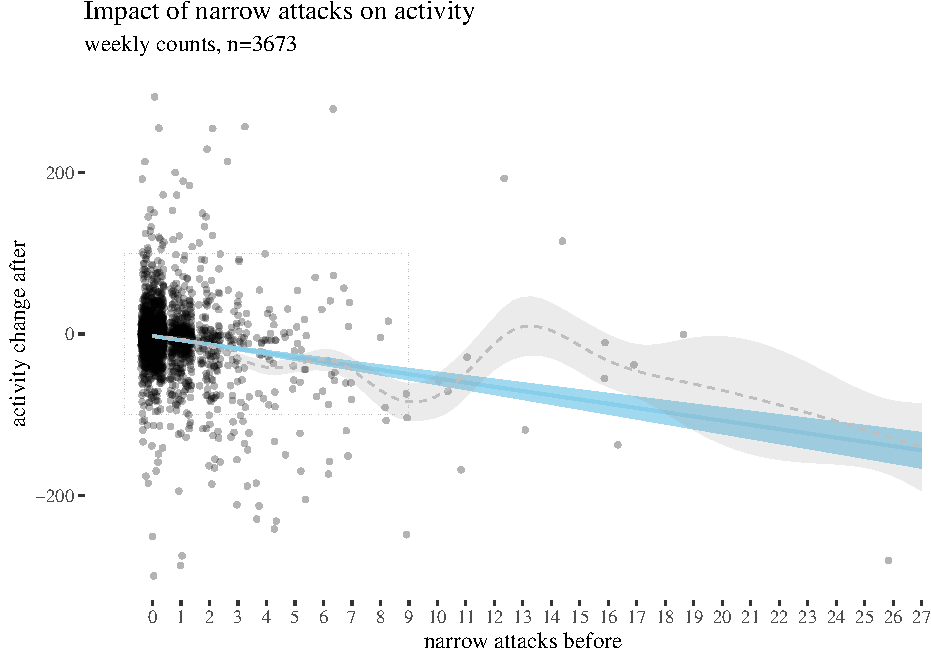
\includegraphics[width=1\linewidth]{redditAnalysisWalkthrough_files/figure-latex/unnamed-chunk-8-1} \end{center}
\caption{Full dataset view (area to be zoomed in is marked).}
\end{subfigure}

\vspace{3mm}
 
\begin{subfigure}[b]{0.95\textwidth}

\begin{center}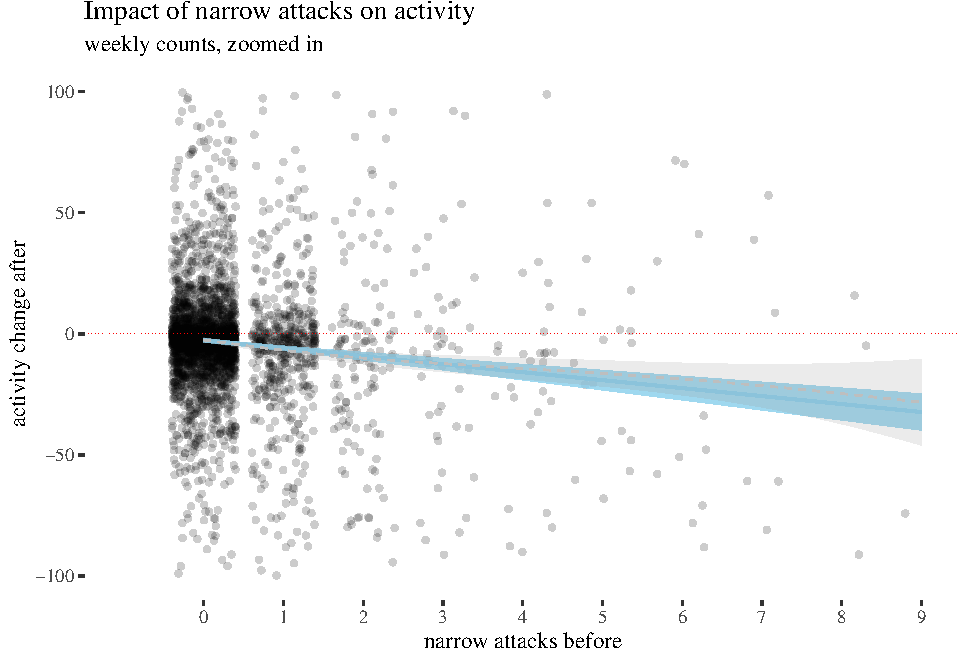
\includegraphics[width=1\linewidth]{redditAnalysisWalkthrough_files/figure-latex/unnamed-chunk-9-1} \end{center}
\caption{Restricted to 0-9 attacks and activity change in the range -100-100, central tendency redrawn, with horizontal reference line at 0.}
\end{subfigure}
\caption{Narrow attacks vs. weekly activity change (jittered), with  linear and gam smoothing.}
\label{fig:highPlots}
\end{figure}

\footnotesize

\begin{Shaded}
\begin{Highlighting}[]
\NormalTok{lowPlot <-}\StringTok{ }\KeywordTok{ggplot}\NormalTok{(data, }\KeywordTok{aes}\NormalTok{(}\DataTypeTok{x =}\NormalTok{ sumLowBefore, }\DataTypeTok{y =}\NormalTok{ activityDiff)) }\OperatorTok{+}
\StringTok{    }\KeywordTok{geom_jitter}\NormalTok{(}\DataTypeTok{size =} \FloatTok{0.8}\NormalTok{, }\DataTypeTok{alpha =} \FloatTok{0.3}\NormalTok{) }\OperatorTok{+}\StringTok{ }\KeywordTok{geom_smooth}\NormalTok{(}\DataTypeTok{method =} \StringTok{"lm"}\NormalTok{,}
    \DataTypeTok{color =} \StringTok{"skyblue"}\NormalTok{, }\DataTypeTok{fill =} \StringTok{"skyblue"}\NormalTok{, }\DataTypeTok{size =} \FloatTok{0.7}\NormalTok{, }\DataTypeTok{alpha =} \FloatTok{0.8}\NormalTok{) }\OperatorTok{+}
\StringTok{    }\NormalTok{th }\OperatorTok{+}\StringTok{ }\KeywordTok{geom_smooth}\NormalTok{(}\DataTypeTok{color =} \StringTok{"grey"}\NormalTok{, }\DataTypeTok{size =} \FloatTok{0.4}\NormalTok{, }\DataTypeTok{lty =} \DecValTok{2}\NormalTok{, }\DataTypeTok{alpha =} \FloatTok{0.2}\NormalTok{) }\OperatorTok{+}
\StringTok{    }\KeywordTok{xlab}\NormalTok{(}\StringTok{"wide attacks before"}\NormalTok{) }\OperatorTok{+}\StringTok{ }\KeywordTok{ylab}\NormalTok{(}\StringTok{"activity change after"}\NormalTok{) }\OperatorTok{+}
\StringTok{    }\KeywordTok{labs}\NormalTok{(}\DataTypeTok{title =} \StringTok{"Impact of wide attacks on activity"}\NormalTok{, }\DataTypeTok{subtitle =} \StringTok{"weekly counts, n=3673"}\NormalTok{) }\OperatorTok{+}
\StringTok{    }\KeywordTok{geom_segment}\NormalTok{(}\KeywordTok{aes}\NormalTok{(}\DataTypeTok{x =} \DecValTok{-1}\NormalTok{, }\DataTypeTok{y =} \DecValTok{-150}\NormalTok{, }\DataTypeTok{xend =} \DecValTok{15}\NormalTok{, }\DataTypeTok{yend =} \DecValTok{-150}\NormalTok{),}
        \DataTypeTok{lty =} \DecValTok{3}\NormalTok{, }\DataTypeTok{size =} \FloatTok{0.1}\NormalTok{, }\DataTypeTok{color =} \StringTok{"gray71"}\NormalTok{, }\DataTypeTok{alpha =} \FloatTok{0.2}\NormalTok{) }\OperatorTok{+}
\StringTok{    }\KeywordTok{geom_segment}\NormalTok{(}\KeywordTok{aes}\NormalTok{(}\DataTypeTok{x =} \DecValTok{-1}\NormalTok{, }\DataTypeTok{y =} \DecValTok{150}\NormalTok{, }\DataTypeTok{xend =} \DecValTok{15}\NormalTok{, }\DataTypeTok{yend =} \DecValTok{150}\NormalTok{),}
        \DataTypeTok{lty =} \DecValTok{3}\NormalTok{, }\DataTypeTok{size =} \FloatTok{0.1}\NormalTok{, }\DataTypeTok{color =} \StringTok{"gray71"}\NormalTok{, }\DataTypeTok{alpha =} \FloatTok{0.2}\NormalTok{) }\OperatorTok{+}
\StringTok{    }\KeywordTok{geom_segment}\NormalTok{(}\KeywordTok{aes}\NormalTok{(}\DataTypeTok{x =} \DecValTok{-1}\NormalTok{, }\DataTypeTok{y =} \DecValTok{-150}\NormalTok{, }\DataTypeTok{xend =} \DecValTok{-1}\NormalTok{, }\DataTypeTok{yend =} \DecValTok{150}\NormalTok{),}
        \DataTypeTok{lty =} \DecValTok{3}\NormalTok{, }\DataTypeTok{size =} \FloatTok{0.1}\NormalTok{, }\DataTypeTok{color =} \StringTok{"gray71"}\NormalTok{, }\DataTypeTok{alpha =} \FloatTok{0.2}\NormalTok{) }\OperatorTok{+}
\StringTok{    }\KeywordTok{geom_segment}\NormalTok{(}\KeywordTok{aes}\NormalTok{(}\DataTypeTok{x =} \DecValTok{15}\NormalTok{, }\DataTypeTok{y =} \DecValTok{-150}\NormalTok{, }\DataTypeTok{xend =} \DecValTok{15}\NormalTok{, }\DataTypeTok{yend =} \DecValTok{150}\NormalTok{),}
        \DataTypeTok{lty =} \DecValTok{3}\NormalTok{, }\DataTypeTok{size =} \FloatTok{0.1}\NormalTok{, }\DataTypeTok{color =} \StringTok{"gray71"}\NormalTok{, }\DataTypeTok{alpha =} \FloatTok{0.2}\NormalTok{) }\OperatorTok{+}
\StringTok{    }\KeywordTok{xlim}\NormalTok{(}\KeywordTok{c}\NormalTok{(}\OperatorTok{-}\DecValTok{1}\NormalTok{, }\KeywordTok{max}\NormalTok{(data}\OperatorTok{$}\NormalTok{sumLowBefore)))}



\NormalTok{lowPlotZoomed <-}\StringTok{ }\KeywordTok{ggplot}\NormalTok{(data, }\KeywordTok{aes}\NormalTok{(}\DataTypeTok{x =}\NormalTok{ sumLowBefore, }\DataTypeTok{y =}\NormalTok{ activityDiff)) }\OperatorTok{+}
\StringTok{    }\KeywordTok{geom_jitter}\NormalTok{(}\DataTypeTok{size =} \DecValTok{1}\NormalTok{, }\DataTypeTok{alpha =} \FloatTok{0.2}\NormalTok{) }\OperatorTok{+}\StringTok{ }\KeywordTok{geom_smooth}\NormalTok{(}\DataTypeTok{method =} \StringTok{"lm"}\NormalTok{,}
    \DataTypeTok{color =} \StringTok{"skyblue"}\NormalTok{, }\DataTypeTok{fill =} \StringTok{"skyblue"}\NormalTok{, }\DataTypeTok{size =} \FloatTok{0.7}\NormalTok{, }\DataTypeTok{alpha =} \FloatTok{0.8}\NormalTok{) }\OperatorTok{+}
\StringTok{    }\NormalTok{th }\OperatorTok{+}\StringTok{ }\KeywordTok{scale_x_continuous}\NormalTok{(}\DataTypeTok{breaks =} \DecValTok{0}\OperatorTok{:}\KeywordTok{max}\NormalTok{(data}\OperatorTok{$}\NormalTok{sumLowBefore),}
    \DataTypeTok{limits =} \KeywordTok{c}\NormalTok{(}\OperatorTok{-}\DecValTok{1}\NormalTok{, }\DecValTok{15}\NormalTok{)) }\OperatorTok{+}\StringTok{ }\KeywordTok{ylim}\NormalTok{(}\KeywordTok{c}\NormalTok{(}\OperatorTok{-}\DecValTok{150}\NormalTok{, }\DecValTok{150}\NormalTok{)) }\OperatorTok{+}\StringTok{ }\KeywordTok{geom_smooth}\NormalTok{(}\DataTypeTok{color =} \StringTok{"grey"}\NormalTok{,}
    \DataTypeTok{size =} \FloatTok{0.4}\NormalTok{, }\DataTypeTok{lty =} \DecValTok{2}\NormalTok{, }\DataTypeTok{alpha =} \FloatTok{0.2}\NormalTok{) }\OperatorTok{+}\StringTok{ }\KeywordTok{xlab}\NormalTok{(}\StringTok{"wide attacks before"}\NormalTok{) }\OperatorTok{+}
\StringTok{    }\KeywordTok{ylab}\NormalTok{(}\StringTok{"activity change after"}\NormalTok{) }\OperatorTok{+}\StringTok{ }\KeywordTok{labs}\NormalTok{(}\DataTypeTok{title =} \StringTok{"Impact of wide attacks on activity"}\NormalTok{,}
    \DataTypeTok{subtitle =} \StringTok{"weekly counts, zoomed in"}\NormalTok{) }\OperatorTok{+}\StringTok{ }\KeywordTok{geom_hline}\NormalTok{(}\DataTypeTok{yintercept =} \DecValTok{0}\NormalTok{,}
    \DataTypeTok{col =} \StringTok{"red"}\NormalTok{, }\DataTypeTok{size =} \FloatTok{0.2}\NormalTok{, }\DataTypeTok{lty =} \DecValTok{3}\NormalTok{)}
\end{Highlighting}
\end{Shaded}

\normalsize

\begin{figure}
\begin{subfigure}[b]{0.95\textwidth}

\begin{center}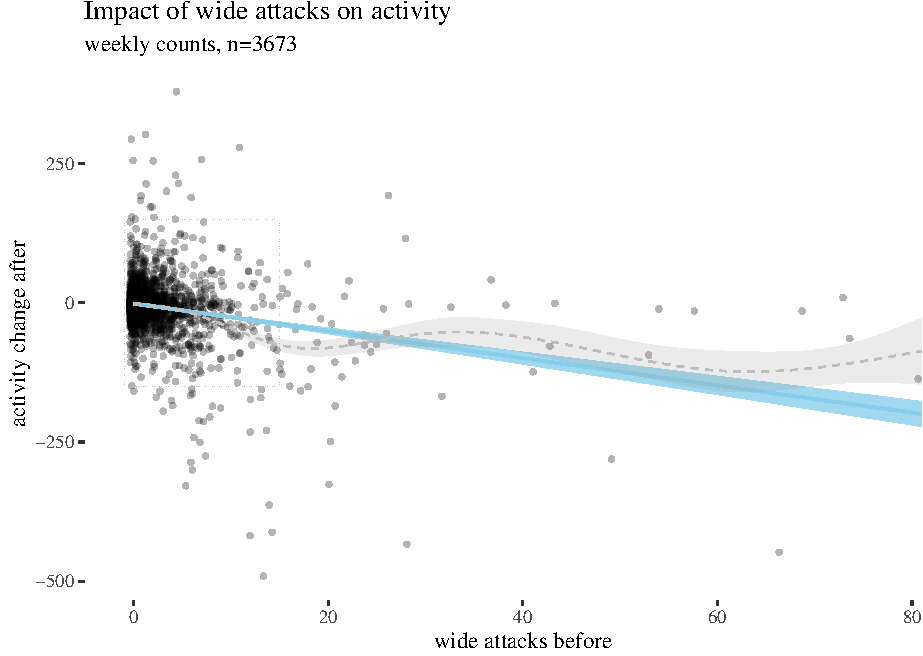
\includegraphics[width=1\linewidth]{redditAnalysisWalkthrough_files/figure-latex/unnamed-chunk-11-1} \end{center}
\caption{Full dataset view (area to be zoomed in is marked).}
\end{subfigure}
 
\begin{subfigure}[b]{0.95\textwidth}

\begin{center}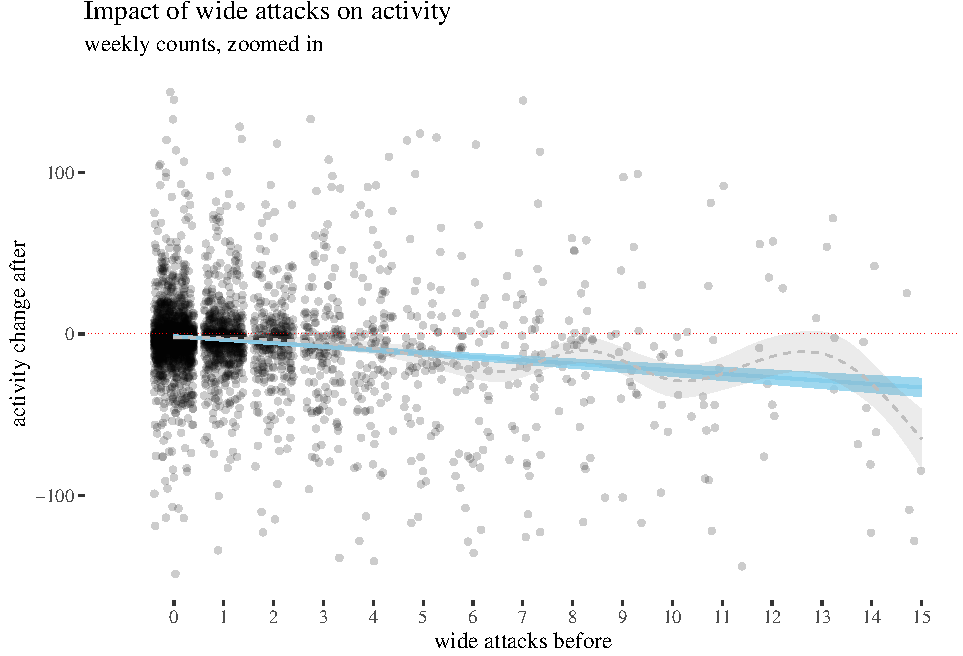
\includegraphics[width=1\linewidth]{redditAnalysisWalkthrough_files/figure-latex/unnamed-chunk-12-1} \end{center}
\caption{Restricted to 0-15 attacks and activity change in the range -150-150, central tendency redrawn, with horizontal reference line at 0.}
\end{subfigure}
\caption{Wide attacks vs. weekly activity change (jittered), with  linear and gam smoothing.}
\label{fig:lowPlots}
\end{figure}

\footnotesize

\begin{Shaded}
\begin{Highlighting}[]
\NormalTok{lowOnlyPlot <-}\StringTok{ }\KeywordTok{ggplot}\NormalTok{(data, }\KeywordTok{aes}\NormalTok{(}\DataTypeTok{x =}\NormalTok{ (sumLowBefore }\OperatorTok{-}\StringTok{ }\NormalTok{sumHighBefore),}
    \DataTypeTok{y =}\NormalTok{ activityDiff)) }\OperatorTok{+}\StringTok{ }\KeywordTok{geom_jitter}\NormalTok{(}\DataTypeTok{size =} \FloatTok{0.8}\NormalTok{, }\DataTypeTok{alpha =} \FloatTok{0.3}\NormalTok{) }\OperatorTok{+}
\StringTok{    }\KeywordTok{geom_smooth}\NormalTok{(}\DataTypeTok{method =} \StringTok{"lm"}\NormalTok{, }\DataTypeTok{color =} \StringTok{"skyblue"}\NormalTok{, }\DataTypeTok{fill =} \StringTok{"skyblue"}\NormalTok{,}
        \DataTypeTok{size =} \FloatTok{0.7}\NormalTok{, }\DataTypeTok{alpha =} \FloatTok{0.8}\NormalTok{) }\OperatorTok{+}\StringTok{ }\NormalTok{th }\OperatorTok{+}\StringTok{ }\KeywordTok{geom_smooth}\NormalTok{(}\DataTypeTok{color =} \StringTok{"grey"}\NormalTok{,}
    \DataTypeTok{size =} \FloatTok{0.4}\NormalTok{, }\DataTypeTok{lty =} \DecValTok{2}\NormalTok{, }\DataTypeTok{alpha =} \FloatTok{0.2}\NormalTok{) }\OperatorTok{+}\StringTok{ }\KeywordTok{xlab}\NormalTok{(}\StringTok{"wide only attacks before"}\NormalTok{) }\OperatorTok{+}
\StringTok{    }\KeywordTok{ylab}\NormalTok{(}\StringTok{"activity change after"}\NormalTok{) }\OperatorTok{+}\StringTok{ }\KeywordTok{labs}\NormalTok{(}\DataTypeTok{title =} \StringTok{"Impact of wide only attacks on activity"}\NormalTok{,}
    \DataTypeTok{subtitle =} \StringTok{"weekly counts, n=3673"}\NormalTok{) }\OperatorTok{+}\StringTok{ }\KeywordTok{geom_segment}\NormalTok{(}\KeywordTok{aes}\NormalTok{(}\DataTypeTok{x =} \DecValTok{-1}\NormalTok{,}
    \DataTypeTok{y =} \DecValTok{-150}\NormalTok{, }\DataTypeTok{xend =} \DecValTok{15}\NormalTok{, }\DataTypeTok{yend =} \DecValTok{-150}\NormalTok{), }\DataTypeTok{lty =} \DecValTok{3}\NormalTok{, }\DataTypeTok{size =} \FloatTok{0.1}\NormalTok{, }\DataTypeTok{color =} \StringTok{"gray71"}\NormalTok{,}
    \DataTypeTok{alpha =} \FloatTok{0.2}\NormalTok{) }\OperatorTok{+}\StringTok{ }\KeywordTok{geom_segment}\NormalTok{(}\KeywordTok{aes}\NormalTok{(}\DataTypeTok{x =} \DecValTok{-1}\NormalTok{, }\DataTypeTok{y =} \DecValTok{150}\NormalTok{, }\DataTypeTok{xend =} \DecValTok{15}\NormalTok{,}
    \DataTypeTok{yend =} \DecValTok{150}\NormalTok{), }\DataTypeTok{lty =} \DecValTok{3}\NormalTok{, }\DataTypeTok{size =} \FloatTok{0.1}\NormalTok{, }\DataTypeTok{color =} \StringTok{"gray71"}\NormalTok{, }\DataTypeTok{alpha =} \FloatTok{0.2}\NormalTok{) }\OperatorTok{+}
\StringTok{    }\KeywordTok{geom_segment}\NormalTok{(}\KeywordTok{aes}\NormalTok{(}\DataTypeTok{x =} \DecValTok{-1}\NormalTok{, }\DataTypeTok{y =} \DecValTok{-150}\NormalTok{, }\DataTypeTok{xend =} \DecValTok{-1}\NormalTok{, }\DataTypeTok{yend =} \DecValTok{150}\NormalTok{),}
        \DataTypeTok{lty =} \DecValTok{3}\NormalTok{, }\DataTypeTok{size =} \FloatTok{0.1}\NormalTok{, }\DataTypeTok{color =} \StringTok{"gray71"}\NormalTok{, }\DataTypeTok{alpha =} \FloatTok{0.2}\NormalTok{) }\OperatorTok{+}
\StringTok{    }\KeywordTok{geom_segment}\NormalTok{(}\KeywordTok{aes}\NormalTok{(}\DataTypeTok{x =} \DecValTok{15}\NormalTok{, }\DataTypeTok{y =} \DecValTok{-150}\NormalTok{, }\DataTypeTok{xend =} \DecValTok{15}\NormalTok{, }\DataTypeTok{yend =} \DecValTok{150}\NormalTok{),}
        \DataTypeTok{lty =} \DecValTok{3}\NormalTok{, }\DataTypeTok{size =} \FloatTok{0.1}\NormalTok{, }\DataTypeTok{color =} \StringTok{"gray71"}\NormalTok{, }\DataTypeTok{alpha =} \FloatTok{0.2}\NormalTok{) }\OperatorTok{+}
\StringTok{    }\KeywordTok{xlim}\NormalTok{(}\KeywordTok{c}\NormalTok{(}\OperatorTok{-}\DecValTok{1}\NormalTok{, }\KeywordTok{max}\NormalTok{(data}\OperatorTok{$}\NormalTok{sumLowBefore)))}


\NormalTok{lowOnlyPlotZoomed <-}\StringTok{ }\KeywordTok{ggplot}\NormalTok{(data, }\KeywordTok{aes}\NormalTok{(}\DataTypeTok{x =}\NormalTok{ (sumLowBefore }\OperatorTok{-}\StringTok{ }\NormalTok{sumHighBefore),}
    \DataTypeTok{y =}\NormalTok{ activityDiff)) }\OperatorTok{+}\StringTok{ }\KeywordTok{geom_jitter}\NormalTok{(}\DataTypeTok{size =} \DecValTok{1}\NormalTok{, }\DataTypeTok{alpha =} \FloatTok{0.2}\NormalTok{) }\OperatorTok{+}
\StringTok{    }\KeywordTok{geom_smooth}\NormalTok{(}\DataTypeTok{method =} \StringTok{"lm"}\NormalTok{, }\DataTypeTok{color =} \StringTok{"skyblue"}\NormalTok{, }\DataTypeTok{fill =} \StringTok{"skyblue"}\NormalTok{,}
        \DataTypeTok{size =} \FloatTok{0.7}\NormalTok{, }\DataTypeTok{alpha =} \FloatTok{0.8}\NormalTok{) }\OperatorTok{+}\StringTok{ }\NormalTok{th }\OperatorTok{+}\StringTok{ }\KeywordTok{scale_x_continuous}\NormalTok{(}\DataTypeTok{breaks =} \DecValTok{0}\OperatorTok{:}\KeywordTok{max}\NormalTok{(data}\OperatorTok{$}\NormalTok{sumLowBefore),}
    \DataTypeTok{limits =} \KeywordTok{c}\NormalTok{(}\OperatorTok{-}\DecValTok{1}\NormalTok{, }\DecValTok{15}\NormalTok{)) }\OperatorTok{+}\StringTok{ }\KeywordTok{ylim}\NormalTok{(}\KeywordTok{c}\NormalTok{(}\OperatorTok{-}\DecValTok{150}\NormalTok{, }\DecValTok{150}\NormalTok{)) }\OperatorTok{+}\StringTok{ }\KeywordTok{geom_smooth}\NormalTok{(}\DataTypeTok{color =} \StringTok{"grey"}\NormalTok{,}
    \DataTypeTok{size =} \FloatTok{0.4}\NormalTok{, }\DataTypeTok{lty =} \DecValTok{2}\NormalTok{, }\DataTypeTok{alpha =} \FloatTok{0.2}\NormalTok{) }\OperatorTok{+}\StringTok{ }\KeywordTok{xlab}\NormalTok{(}\StringTok{"wide only attacks before"}\NormalTok{) }\OperatorTok{+}
\StringTok{    }\KeywordTok{ylab}\NormalTok{(}\StringTok{"activity change after"}\NormalTok{) }\OperatorTok{+}\StringTok{ }\KeywordTok{labs}\NormalTok{(}\DataTypeTok{title =} \StringTok{"Impact of wide only attacks on activity"}\NormalTok{,}
    \DataTypeTok{subtitle =} \StringTok{"weekly counts, zoomed in"}\NormalTok{) }\OperatorTok{+}\StringTok{ }\KeywordTok{geom_hline}\NormalTok{(}\DataTypeTok{yintercept =} \DecValTok{0}\NormalTok{,}
    \DataTypeTok{col =} \StringTok{"red"}\NormalTok{, }\DataTypeTok{size =} \FloatTok{0.2}\NormalTok{, }\DataTypeTok{lty =} \DecValTok{3}\NormalTok{)}
\end{Highlighting}
\end{Shaded}

\normalsize

\begin{figure}
\Centering
\begin{subfigure}[b]{0.95\textwidth}

\begin{center}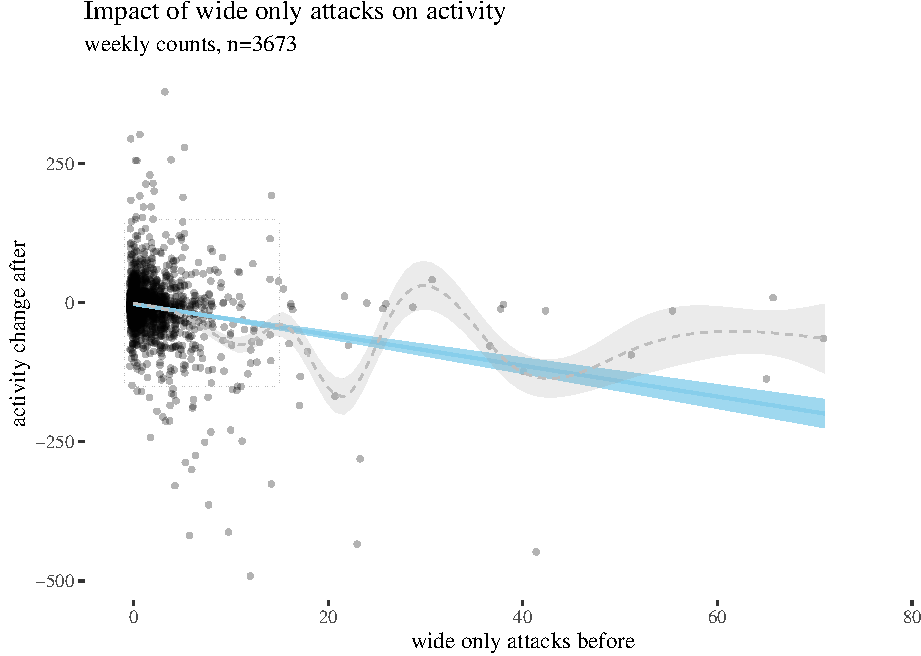
\includegraphics[width=1\linewidth]{redditAnalysisWalkthrough_files/figure-latex/unnamed-chunk-14-1} \end{center}
\caption{Full dataset view (area to be zoomed in is marked).}
\end{subfigure}
 
\begin{subfigure}[b]{0.95\textwidth}

\begin{center}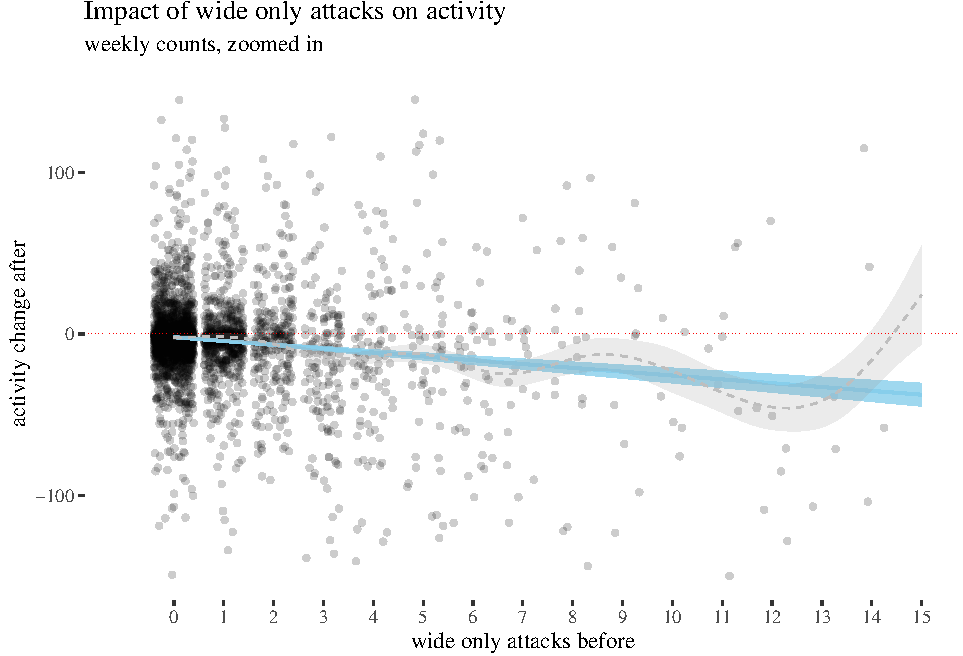
\includegraphics[width=1\linewidth]{redditAnalysisWalkthrough_files/figure-latex/unnamed-chunk-15-1} \end{center}
\caption{Restricted to 0-15 attacks and activity change in the range -150-150, central tendency redrawn, with horizontal reference line at 0.}
\end{subfigure}
\caption{Wide only attacks vs. weekly activity change (jittered), with  linear and gam smoothing.}
\label{fig:lowOnlyPlots}
\end{figure}

The above visualises the activity change in terms of weekly counts.
However, arguably, a change of -20 for a user who posts 500 times a week
has different weight than for a user who posts 30 times. For this
reason, we also need to look at changes in proportion, calculated by the
following formula:

\begin{align}
\mathsf{activityScore} = & \frac{\mathsf{activityDifference}}{\mathsf{activityBefore}}
\end{align}

We zoom in to densely populated areas of the plot for
\textsf{activityScore} as a function of the three types of attacks in
Figure \ref{fig:propActivity}. The impact is still negative, more so for
\textsf{narrow} attacks, and less so for other types. Note that for
mathematical reasons the score minimum is -1 (user activity cannot drop
more than 100\%), and so the graph looks assymetric around the
horizontal line.

\footnotesize

\begin{Shaded}
\begin{Highlighting}[]
\NormalTok{rescale <-}\StringTok{ }\ControlFlowTok{function}\NormalTok{(diff, act) \{}
\NormalTok{    diff}\OperatorTok{/}\NormalTok{act}
\NormalTok{\}}
\NormalTok{data}\OperatorTok{$}\NormalTok{activityScore <-}\StringTok{ }\KeywordTok{rescale}\NormalTok{(data}\OperatorTok{$}\NormalTok{activityDiff, data}\OperatorTok{$}\NormalTok{activityBefore)}

\NormalTok{propPlotHigh <-}\StringTok{ }\KeywordTok{ggplot}\NormalTok{(data, }\KeywordTok{aes}\NormalTok{(}\DataTypeTok{x =}\NormalTok{ sumHighBefore, }\DataTypeTok{y =}\NormalTok{ activityScore)) }\OperatorTok{+}
\StringTok{    }\KeywordTok{geom_jitter}\NormalTok{(}\DataTypeTok{size =} \FloatTok{0.8}\NormalTok{, }\DataTypeTok{alpha =} \FloatTok{0.3}\NormalTok{) }\OperatorTok{+}\StringTok{ }\KeywordTok{geom_smooth}\NormalTok{(}\DataTypeTok{method =} \StringTok{"lm"}\NormalTok{,}
    \DataTypeTok{color =} \StringTok{"skyblue"}\NormalTok{, }\DataTypeTok{fill =} \StringTok{"skyblue"}\NormalTok{, }\DataTypeTok{size =} \FloatTok{0.7}\NormalTok{, }\DataTypeTok{alpha =} \FloatTok{0.8}\NormalTok{) }\OperatorTok{+}
\StringTok{    }\NormalTok{th }\OperatorTok{+}\StringTok{ }\KeywordTok{xlab}\NormalTok{(}\StringTok{"narrow attacks before"}\NormalTok{) }\OperatorTok{+}\StringTok{ }\KeywordTok{ylab}\NormalTok{(}\StringTok{"proportional activity change"}\NormalTok{) }\OperatorTok{+}
\StringTok{    }\KeywordTok{labs}\NormalTok{(}\DataTypeTok{title =} \StringTok{"Impact of narrow attacks on proportional activity"}\NormalTok{,}
        \DataTypeTok{subtitle =} \StringTok{"n=3673"}\NormalTok{) }\OperatorTok{+}\StringTok{ }\KeywordTok{scale_y_continuous}\NormalTok{(}\DataTypeTok{limits =} \KeywordTok{c}\NormalTok{(}\OperatorTok{-}\DecValTok{1}\NormalTok{,}
    \DecValTok{10}\NormalTok{)) }\OperatorTok{+}\StringTok{ }\KeywordTok{geom_hline}\NormalTok{(}\DataTypeTok{yintercept =} \DecValTok{0}\NormalTok{, }\DataTypeTok{col =} \StringTok{"red"}\NormalTok{, }\DataTypeTok{size =} \FloatTok{0.2}\NormalTok{,}
    \DataTypeTok{lty =} \DecValTok{3}\NormalTok{) }\OperatorTok{+}\StringTok{ }\KeywordTok{scale_x_continuous}\NormalTok{(}\DataTypeTok{breaks =} \DecValTok{1}\OperatorTok{:}\DecValTok{15}\NormalTok{, }\DataTypeTok{limits =} \KeywordTok{c}\NormalTok{(}\OperatorTok{-}\DecValTok{1}\NormalTok{,}
    \DecValTok{10}\NormalTok{)) }\OperatorTok{+}\StringTok{ }\KeywordTok{geom_smooth}\NormalTok{(}\DataTypeTok{color =} \StringTok{"grey"}\NormalTok{, }\DataTypeTok{size =} \FloatTok{0.4}\NormalTok{, }\DataTypeTok{lty =} \DecValTok{2}\NormalTok{, }\DataTypeTok{alpha =} \FloatTok{0.2}\NormalTok{)}

\NormalTok{propPlotLow <-}\StringTok{ }\KeywordTok{ggplot}\NormalTok{(data, }\KeywordTok{aes}\NormalTok{(}\DataTypeTok{x =}\NormalTok{ sumLowBefore, }\DataTypeTok{y =}\NormalTok{ activityScore)) }\OperatorTok{+}
\StringTok{    }\KeywordTok{geom_jitter}\NormalTok{(}\DataTypeTok{size =} \FloatTok{0.8}\NormalTok{, }\DataTypeTok{alpha =} \FloatTok{0.3}\NormalTok{) }\OperatorTok{+}\StringTok{ }\KeywordTok{geom_smooth}\NormalTok{(}\DataTypeTok{method =} \StringTok{"lm"}\NormalTok{,}
    \DataTypeTok{color =} \StringTok{"skyblue"}\NormalTok{, }\DataTypeTok{fill =} \StringTok{"skyblue"}\NormalTok{, }\DataTypeTok{size =} \FloatTok{0.7}\NormalTok{, }\DataTypeTok{alpha =} \FloatTok{0.8}\NormalTok{) }\OperatorTok{+}
\StringTok{    }\NormalTok{th }\OperatorTok{+}\StringTok{ }\KeywordTok{xlab}\NormalTok{(}\StringTok{"wide attacks before"}\NormalTok{) }\OperatorTok{+}\StringTok{ }\KeywordTok{ylab}\NormalTok{(}\StringTok{"proportional activity change"}\NormalTok{) }\OperatorTok{+}
\StringTok{    }\KeywordTok{labs}\NormalTok{(}\DataTypeTok{title =} \StringTok{"Impact of wide attacks on proportional activity"}\NormalTok{,}
        \DataTypeTok{subtitle =} \StringTok{"n=3673"}\NormalTok{) }\OperatorTok{+}\StringTok{ }\KeywordTok{scale_y_continuous}\NormalTok{(}\DataTypeTok{limits =} \KeywordTok{c}\NormalTok{(}\OperatorTok{-}\DecValTok{1}\NormalTok{,}
    \DecValTok{10}\NormalTok{)) }\OperatorTok{+}\StringTok{ }\KeywordTok{geom_hline}\NormalTok{(}\DataTypeTok{yintercept =} \DecValTok{0}\NormalTok{, }\DataTypeTok{col =} \StringTok{"red"}\NormalTok{, }\DataTypeTok{size =} \FloatTok{0.2}\NormalTok{,}
    \DataTypeTok{lty =} \DecValTok{3}\NormalTok{) }\OperatorTok{+}\StringTok{ }\KeywordTok{scale_x_continuous}\NormalTok{(}\DataTypeTok{breaks =} \DecValTok{1}\OperatorTok{:}\DecValTok{15}\NormalTok{, }\DataTypeTok{limits =} \KeywordTok{c}\NormalTok{(}\OperatorTok{-}\DecValTok{1}\NormalTok{,}
    \DecValTok{10}\NormalTok{)) }\OperatorTok{+}\StringTok{ }\KeywordTok{geom_smooth}\NormalTok{(}\DataTypeTok{color =} \StringTok{"grey"}\NormalTok{, }\DataTypeTok{size =} \FloatTok{0.4}\NormalTok{, }\DataTypeTok{lty =} \DecValTok{2}\NormalTok{, }\DataTypeTok{alpha =} \FloatTok{0.2}\NormalTok{)}


\NormalTok{propPlotLowOnly <-}\StringTok{ }\KeywordTok{ggplot}\NormalTok{(data, }\KeywordTok{aes}\NormalTok{(}\DataTypeTok{x =}\NormalTok{ sumLowBefore }\OperatorTok{-}\StringTok{ }\NormalTok{sumHighBefore,}
    \DataTypeTok{y =}\NormalTok{ activityScore)) }\OperatorTok{+}\StringTok{ }\KeywordTok{geom_jitter}\NormalTok{(}\DataTypeTok{size =} \FloatTok{0.8}\NormalTok{, }\DataTypeTok{alpha =} \FloatTok{0.3}\NormalTok{) }\OperatorTok{+}
\StringTok{    }\KeywordTok{geom_smooth}\NormalTok{(}\DataTypeTok{method =} \StringTok{"lm"}\NormalTok{, }\DataTypeTok{color =} \StringTok{"skyblue"}\NormalTok{, }\DataTypeTok{fill =} \StringTok{"skyblue"}\NormalTok{,}
        \DataTypeTok{size =} \FloatTok{0.7}\NormalTok{, }\DataTypeTok{alpha =} \FloatTok{0.8}\NormalTok{) }\OperatorTok{+}\StringTok{ }\NormalTok{th }\OperatorTok{+}\StringTok{ }\KeywordTok{xlab}\NormalTok{(}\StringTok{"wide only attacks before"}\NormalTok{) }\OperatorTok{+}
\StringTok{    }\KeywordTok{ylab}\NormalTok{(}\StringTok{"proportional activity change"}\NormalTok{) }\OperatorTok{+}\StringTok{ }\KeywordTok{labs}\NormalTok{(}\DataTypeTok{title =} \StringTok{"Impact of wide only attacks on proportional activity"}\NormalTok{,}
    \DataTypeTok{subtitle =} \StringTok{"n=3673"}\NormalTok{) }\OperatorTok{+}\StringTok{ }\KeywordTok{scale_y_continuous}\NormalTok{(}\DataTypeTok{limits =} \KeywordTok{c}\NormalTok{(}\OperatorTok{-}\DecValTok{1}\NormalTok{,}
    \DecValTok{10}\NormalTok{)) }\OperatorTok{+}\StringTok{ }\KeywordTok{geom_hline}\NormalTok{(}\DataTypeTok{yintercept =} \DecValTok{0}\NormalTok{, }\DataTypeTok{col =} \StringTok{"red"}\NormalTok{, }\DataTypeTok{size =} \FloatTok{0.2}\NormalTok{,}
    \DataTypeTok{lty =} \DecValTok{3}\NormalTok{) }\OperatorTok{+}\StringTok{ }\KeywordTok{scale_x_continuous}\NormalTok{(}\DataTypeTok{breaks =} \DecValTok{1}\OperatorTok{:}\DecValTok{15}\NormalTok{, }\DataTypeTok{limits =} \KeywordTok{c}\NormalTok{(}\OperatorTok{-}\DecValTok{1}\NormalTok{,}
    \DecValTok{10}\NormalTok{)) }\OperatorTok{+}\StringTok{ }\KeywordTok{geom_smooth}\NormalTok{(}\DataTypeTok{color =} \StringTok{"grey"}\NormalTok{, }\DataTypeTok{size =} \FloatTok{0.4}\NormalTok{, }\DataTypeTok{lty =} \DecValTok{2}\NormalTok{, }\DataTypeTok{alpha =} \FloatTok{0.2}\NormalTok{)}
\end{Highlighting}
\end{Shaded}

\normalsize

\begin{figure}
\begin{subfigure}[b]{0.75\textwidth}

\begin{center}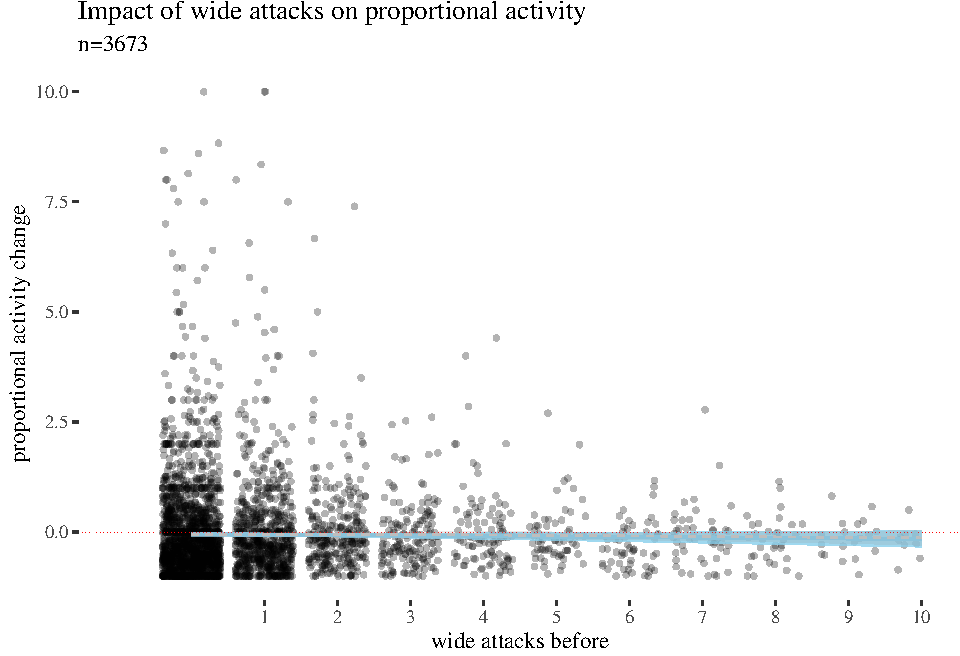
\includegraphics[width=1\linewidth]{redditAnalysisWalkthrough_files/figure-latex/unnamed-chunk-17-1} \end{center}
\end{subfigure}
 
 \vspace{3mm}
\begin{subfigure}[b]{0.75\textwidth}

\begin{center}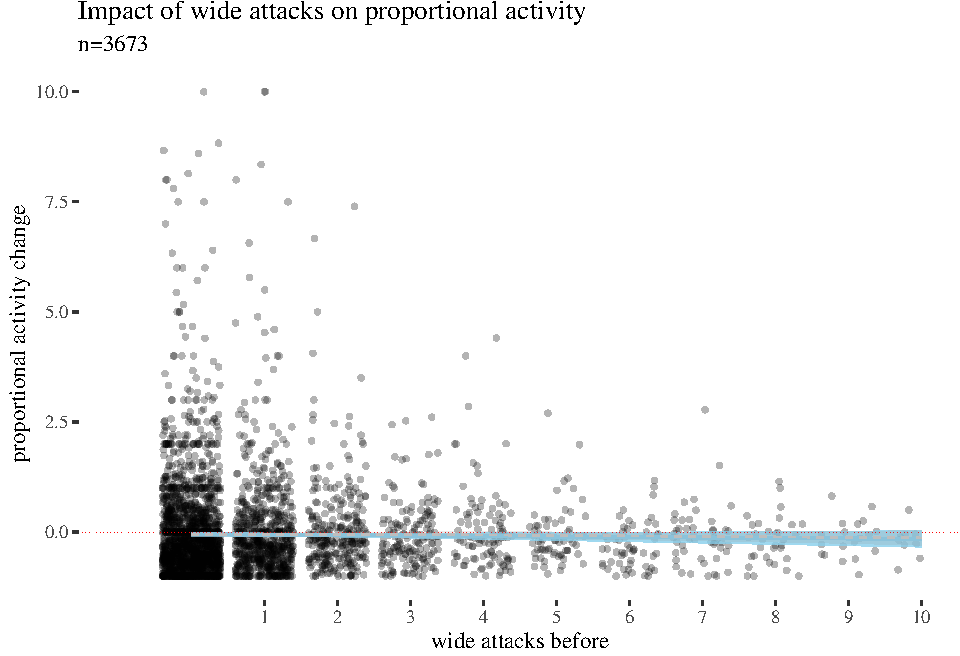
\includegraphics[width=1\linewidth]{redditAnalysisWalkthrough_files/figure-latex/unnamed-chunk-18-1} \end{center}
\end{subfigure}


\vspace{3mm}
\begin{subfigure}[b]{0.75\textwidth}

\begin{center}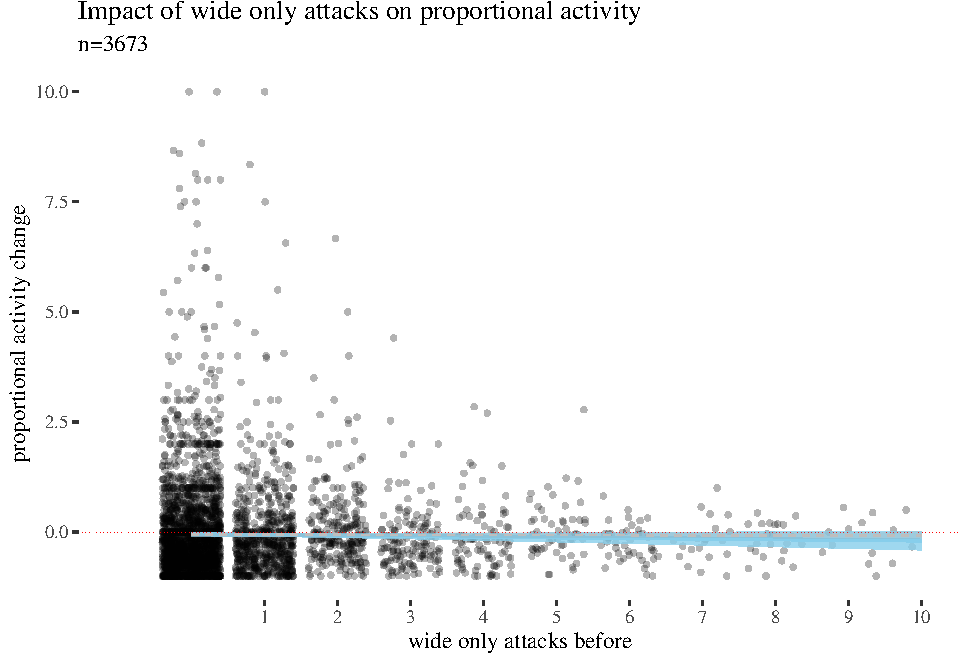
\includegraphics[width=1\linewidth]{redditAnalysisWalkthrough_files/figure-latex/unnamed-chunk-19-1} \end{center}

\end{subfigure}


\caption{Impact of attacks of three types on proportional activity change.}
\label{fig:propActivity}
\end{figure}

\section{Classical estimation}

Next, we focus on the uncertainties involved. One standard way to
estimate them is to use a one-sample t-tests to estimate the means and
95\% confidence intervals for \textsf{activityDifference} for different
numbers of attacks (this would be equivalent to running a paired t-test
for activity before and activity after).

Here is the analysis for narrow attacks. There were not enough
observations for attacks above 8 (3, 2, and 2 for 9, 10 and 11 attacks,
and single observations for a few higher non-zero counts) for a t-test
to be useful, so we run the t-test for up to 8 attacks.

\footnotesize

\begin{table}
\centering\begingroup\fontsize{9}{11}\selectfont

\resizebox{\linewidth}{!}{
\begin{tabular}{lrrrrrrrrrrrrrrrrrrrrr}
\toprule
\cellcolor{gray!6}{no. of attacks} & \cellcolor{gray!6}{0} & \cellcolor{gray!6}{1} & \cellcolor{gray!6}{2} & \cellcolor{gray!6}{3} & \cellcolor{gray!6}{4} & \cellcolor{gray!6}{5} & \cellcolor{gray!6}{6} & \cellcolor{gray!6}{7} & \cellcolor{gray!6}{8} & \cellcolor{gray!6}{9} & \cellcolor{gray!6}{10} & \cellcolor{gray!6}{11} & \cellcolor{gray!6}{12} & \cellcolor{gray!6}{13} & \cellcolor{gray!6}{14} & \cellcolor{gray!6}{16} & \cellcolor{gray!6}{17} & \cellcolor{gray!6}{19} & \cellcolor{gray!6}{25} & \cellcolor{gray!6}{26} & \cellcolor{gray!6}{27}\\
count & 2831 & 530 & 147 & 61 & 35 & 22 & 17 & 8 & 4 & 3 & 2 & 2 & 1 & 1 & 1 & 3 & 1 & 1 & 1 & 1 & 1\\
\bottomrule
\end{tabular}}
\endgroup{}
\end{table}

\normalsize 

We proceed as follows. We list 9 options of the number of attacks and
initiate vectors to which we will save the confidence interval limits
(\textsf{low}, \textsf{high}), the estimated mean and the
\textsf{p}-value. We use the same approach to analyze the other types of
attacks.

\footnotesize

\begin{Shaded}
\begin{Highlighting}[]
\NormalTok{attacks <-}\StringTok{ }\DecValTok{0}\OperatorTok{:}\DecValTok{8}
\NormalTok{max <-}\StringTok{ }\KeywordTok{max}\NormalTok{(attacks)}
\NormalTok{low <-}\StringTok{ }\KeywordTok{numeric}\NormalTok{(max }\OperatorTok{+}\StringTok{ }\DecValTok{1}\NormalTok{)}
\NormalTok{high <-}\StringTok{ }\KeywordTok{numeric}\NormalTok{(max }\OperatorTok{+}\StringTok{ }\DecValTok{1}\NormalTok{)}
\NormalTok{m <-}\StringTok{ }\KeywordTok{numeric}\NormalTok{(max }\OperatorTok{+}\StringTok{ }\DecValTok{1}\NormalTok{)}
\NormalTok{p <-}\StringTok{ }\KeywordTok{numeric}\NormalTok{(max }\OperatorTok{+}\StringTok{ }\DecValTok{1}\NormalTok{)}
\NormalTok{t <-}\StringTok{ }\KeywordTok{list}\NormalTok{()}

\ControlFlowTok{for}\NormalTok{ (attacks }\ControlFlowTok{in}\NormalTok{ attacks) \{}
\NormalTok{    t[[attacks }\OperatorTok{+}\StringTok{ }\DecValTok{1}\NormalTok{]] <-}\StringTok{ }\KeywordTok{t.test}\NormalTok{(data[data}\OperatorTok{$}\NormalTok{sumHighBefore }\OperatorTok{==}\StringTok{ }\NormalTok{attacks,}
\NormalTok{        ]}\OperatorTok{$}\NormalTok{activityDiff)}

\NormalTok{    low[attacks }\OperatorTok{+}\StringTok{ }\DecValTok{1}\NormalTok{] <-}\StringTok{ }\NormalTok{t[[attacks }\OperatorTok{+}\StringTok{ }\DecValTok{1}\NormalTok{]]}\OperatorTok{$}\NormalTok{conf.int[}\DecValTok{1}\NormalTok{]}
\NormalTok{    high[attacks }\OperatorTok{+}\StringTok{ }\DecValTok{1}\NormalTok{] <-}\StringTok{ }\NormalTok{t[[attacks }\OperatorTok{+}\StringTok{ }\DecValTok{1}\NormalTok{]]}\OperatorTok{$}\NormalTok{conf.int[}\DecValTok{2}\NormalTok{]}
\NormalTok{    m[attacks }\OperatorTok{+}\StringTok{ }\DecValTok{1}\NormalTok{] <-}\StringTok{ }\NormalTok{t[[attacks }\OperatorTok{+}\StringTok{ }\DecValTok{1}\NormalTok{]]}\OperatorTok{$}\NormalTok{estimate}
\NormalTok{    p[attacks }\OperatorTok{+}\StringTok{ }\DecValTok{1}\NormalTok{] <-}\StringTok{ }\NormalTok{t[[attacks }\OperatorTok{+}\StringTok{ }\DecValTok{1}\NormalTok{]]}\OperatorTok{$}\NormalTok{p.value}
\NormalTok{\}}
\NormalTok{highTable <-}\StringTok{ }\KeywordTok{as.data.frame}\NormalTok{(}\KeywordTok{round}\NormalTok{(}\KeywordTok{rbind}\NormalTok{(}\DecValTok{0}\OperatorTok{:}\DecValTok{8}\NormalTok{, low, m, high, p),}
    \DecValTok{3}\NormalTok{))}
\KeywordTok{rownames}\NormalTok{(highTable) <-}\StringTok{ }\KeywordTok{c}\NormalTok{(}\StringTok{"attacks"}\NormalTok{, }\StringTok{"CIlow"}\NormalTok{, }\StringTok{"estimated m"}\NormalTok{, }\StringTok{"CIhigh"}\NormalTok{,}
    \StringTok{"p-value"}\NormalTok{)}
\end{Highlighting}
\end{Shaded}

\begin{Shaded}
\begin{Highlighting}[]
\NormalTok{highTableLong <-}\StringTok{ }\KeywordTok{round}\NormalTok{(}\KeywordTok{data.frame}\NormalTok{(}\DataTypeTok{attacks =} \DecValTok{0}\OperatorTok{:}\DecValTok{8}\NormalTok{, low, m, high,}
\NormalTok{    p), }\DecValTok{3}\NormalTok{)}

\NormalTok{highTableBar <-}\StringTok{ }\KeywordTok{ggplot}\NormalTok{(highTableLong) }\OperatorTok{+}\StringTok{ }\KeywordTok{geom_bar}\NormalTok{(}\KeywordTok{aes}\NormalTok{(}\DataTypeTok{x =}\NormalTok{ attacks,}
    \DataTypeTok{y =}\NormalTok{ m), }\DataTypeTok{stat =} \StringTok{"identity"}\NormalTok{, }\DataTypeTok{fill =} \StringTok{"skyblue"}\NormalTok{, }\DataTypeTok{alpha =} \FloatTok{0.5}\NormalTok{) }\OperatorTok{+}
\StringTok{    }\KeywordTok{geom_errorbar}\NormalTok{(}\KeywordTok{aes}\NormalTok{(}\DataTypeTok{x =}\NormalTok{ attacks, }\DataTypeTok{ymin =}\NormalTok{ low, }\DataTypeTok{ymax =}\NormalTok{ high),}
        \DataTypeTok{width =} \FloatTok{0.4}\NormalTok{, }\DataTypeTok{colour =} \StringTok{"seashell3"}\NormalTok{, }\DataTypeTok{alpha =} \FloatTok{0.9}\NormalTok{, }\DataTypeTok{size =} \FloatTok{0.3}\NormalTok{) }\OperatorTok{+}
\StringTok{    }\NormalTok{th }\OperatorTok{+}\StringTok{ }\KeywordTok{xlab}\NormalTok{(}\StringTok{"narrow attacks"}\NormalTok{) }\OperatorTok{+}\StringTok{ }\KeywordTok{ylab}\NormalTok{(}\StringTok{"mean activity change"}\NormalTok{) }\OperatorTok{+}
\StringTok{    }\KeywordTok{geom_text}\NormalTok{(}\KeywordTok{aes}\NormalTok{(}\DataTypeTok{x =}\NormalTok{ attacks, }\DataTypeTok{y =}\NormalTok{ low }\OperatorTok{-}\StringTok{ }\DecValTok{20}\NormalTok{, }\DataTypeTok{label =}\NormalTok{ p), }\DataTypeTok{size =} \DecValTok{2}\NormalTok{) }\OperatorTok{+}
\StringTok{    }\KeywordTok{labs}\NormalTok{(}\DataTypeTok{title =} \StringTok{"Mean impact of narrow attacks on  weekly activity"}\NormalTok{,}
        \DataTypeTok{subtitle =} \StringTok{"with 95% confidence intervals and p-values"}\NormalTok{) }\OperatorTok{+}
\StringTok{    }\KeywordTok{scale_x_continuous}\NormalTok{(}\DataTypeTok{labels =} \DecValTok{0}\OperatorTok{:}\DecValTok{8}\NormalTok{, }\DataTypeTok{breaks =} \DecValTok{0}\OperatorTok{:}\DecValTok{8}\NormalTok{)}

\NormalTok{highTableBar6 <-}\StringTok{ }\KeywordTok{ggplot}\NormalTok{(highTableLong[highTableLong}\OperatorTok{$}\NormalTok{attacks }\OperatorTok{<}
\StringTok{    }\DecValTok{6}\NormalTok{, ]) }\OperatorTok{+}\StringTok{ }\KeywordTok{geom_bar}\NormalTok{(}\KeywordTok{aes}\NormalTok{(}\DataTypeTok{x =}\NormalTok{ attacks, }\DataTypeTok{y =}\NormalTok{ m), }\DataTypeTok{stat =} \StringTok{"identity"}\NormalTok{,}
    \DataTypeTok{fill =} \StringTok{"skyblue"}\NormalTok{, }\DataTypeTok{alpha =} \FloatTok{0.5}\NormalTok{) }\OperatorTok{+}\StringTok{ }\KeywordTok{geom_errorbar}\NormalTok{(}\KeywordTok{aes}\NormalTok{(}\DataTypeTok{x =}\NormalTok{ attacks,}
    \DataTypeTok{ymin =}\NormalTok{ low, }\DataTypeTok{ymax =}\NormalTok{ high), }\DataTypeTok{width =} \FloatTok{0.4}\NormalTok{, }\DataTypeTok{colour =} \StringTok{"seashell3"}\NormalTok{,}
    \DataTypeTok{alpha =} \FloatTok{0.9}\NormalTok{, }\DataTypeTok{size =} \FloatTok{0.3}\NormalTok{) }\OperatorTok{+}\StringTok{ }\NormalTok{th }\OperatorTok{+}\StringTok{ }\KeywordTok{xlab}\NormalTok{(}\StringTok{"narrow attacks"}\NormalTok{) }\OperatorTok{+}
\StringTok{    }\KeywordTok{ylab}\NormalTok{(}\StringTok{"mean activity change"}\NormalTok{) }\OperatorTok{+}\StringTok{ }\KeywordTok{geom_text}\NormalTok{(}\KeywordTok{aes}\NormalTok{(}\DataTypeTok{x =}\NormalTok{ attacks,}
    \DataTypeTok{y =}\NormalTok{ low }\OperatorTok{-}\StringTok{ }\DecValTok{20}\NormalTok{, }\DataTypeTok{label =}\NormalTok{ p), }\DataTypeTok{size =} \DecValTok{2}\NormalTok{) }\OperatorTok{+}\StringTok{ }\KeywordTok{labs}\NormalTok{(}\DataTypeTok{title =} \StringTok{"Mean impact of narrow attacks <6 on  weekly activity"}\NormalTok{,}
    \DataTypeTok{subtitle =} \StringTok{"with 95% confidence intervals and p-values"}\NormalTok{) }\OperatorTok{+}
\StringTok{    }\KeywordTok{scale_x_continuous}\NormalTok{(}\DataTypeTok{labels =} \DecValTok{0}\OperatorTok{:}\DecValTok{5}\NormalTok{, }\DataTypeTok{breaks =} \DecValTok{0}\OperatorTok{:}\DecValTok{5}\NormalTok{)}

\NormalTok{highTableBar3 <-}\StringTok{ }\KeywordTok{ggplot}\NormalTok{(highTableLong[highTableLong}\OperatorTok{$}\NormalTok{attacks }\OperatorTok{<}
\StringTok{    }\DecValTok{3}\NormalTok{, ]) }\OperatorTok{+}\StringTok{ }\KeywordTok{geom_bar}\NormalTok{(}\KeywordTok{aes}\NormalTok{(}\DataTypeTok{x =}\NormalTok{ attacks, }\DataTypeTok{y =}\NormalTok{ m), }\DataTypeTok{stat =} \StringTok{"identity"}\NormalTok{,}
    \DataTypeTok{fill =} \StringTok{"skyblue"}\NormalTok{, }\DataTypeTok{alpha =} \FloatTok{0.5}\NormalTok{) }\OperatorTok{+}\StringTok{ }\KeywordTok{geom_errorbar}\NormalTok{(}\KeywordTok{aes}\NormalTok{(}\DataTypeTok{x =}\NormalTok{ attacks,}
    \DataTypeTok{ymin =}\NormalTok{ low, }\DataTypeTok{ymax =}\NormalTok{ high), }\DataTypeTok{width =} \FloatTok{0.4}\NormalTok{, }\DataTypeTok{colour =} \StringTok{"seashell3"}\NormalTok{,}
    \DataTypeTok{alpha =} \FloatTok{0.9}\NormalTok{, }\DataTypeTok{size =} \FloatTok{0.3}\NormalTok{) }\OperatorTok{+}\StringTok{ }\NormalTok{th }\OperatorTok{+}\StringTok{ }\KeywordTok{xlab}\NormalTok{(}\StringTok{"narrow attacks"}\NormalTok{) }\OperatorTok{+}
\StringTok{    }\KeywordTok{ylab}\NormalTok{(}\StringTok{"mean activity change"}\NormalTok{) }\OperatorTok{+}\StringTok{ }\KeywordTok{geom_text}\NormalTok{(}\KeywordTok{aes}\NormalTok{(}\DataTypeTok{x =}\NormalTok{ attacks,}
    \DataTypeTok{y =}\NormalTok{ low }\OperatorTok{-}\StringTok{ }\DecValTok{5}\NormalTok{, }\DataTypeTok{label =}\NormalTok{ p), }\DataTypeTok{size =} \DecValTok{2}\NormalTok{) }\OperatorTok{+}\StringTok{ }\KeywordTok{labs}\NormalTok{(}\DataTypeTok{title =} \StringTok{"Mean impact of narrow attacks <3 on  weekly activity"}\NormalTok{,}
    \DataTypeTok{subtitle =} \StringTok{"with 95% confidence intervals and p-values"}\NormalTok{) }\OperatorTok{+}
\StringTok{    }\KeywordTok{scale_x_continuous}\NormalTok{(}\DataTypeTok{labels =} \DecValTok{0}\OperatorTok{:}\DecValTok{2}\NormalTok{, }\DataTypeTok{breaks =} \DecValTok{0}\OperatorTok{:}\DecValTok{2}\NormalTok{)}
\end{Highlighting}
\end{Shaded}

\footnotesize

\begin{Shaded}
\begin{Highlighting}[]
\NormalTok{attacks <-}\StringTok{ }\DecValTok{0}\OperatorTok{:}\DecValTok{8}
\NormalTok{max <-}\StringTok{ }\KeywordTok{max}\NormalTok{(attacks)}
\NormalTok{lowL <-}\StringTok{ }\KeywordTok{numeric}\NormalTok{(max }\OperatorTok{+}\StringTok{ }\DecValTok{1}\NormalTok{)}
\NormalTok{highL <-}\StringTok{ }\KeywordTok{numeric}\NormalTok{(max }\OperatorTok{+}\StringTok{ }\DecValTok{1}\NormalTok{)}
\NormalTok{mL <-}\StringTok{ }\KeywordTok{numeric}\NormalTok{(max }\OperatorTok{+}\StringTok{ }\DecValTok{1}\NormalTok{)}
\NormalTok{pL <-}\StringTok{ }\KeywordTok{numeric}\NormalTok{(max }\OperatorTok{+}\StringTok{ }\DecValTok{1}\NormalTok{)}
\NormalTok{tL <-}\StringTok{ }\KeywordTok{list}\NormalTok{()}

\ControlFlowTok{for}\NormalTok{ (attacks }\ControlFlowTok{in}\NormalTok{ attacks) \{}
\NormalTok{    tL[[attacks }\OperatorTok{+}\StringTok{ }\DecValTok{1}\NormalTok{]] <-}\StringTok{ }\KeywordTok{t.test}\NormalTok{(data[data}\OperatorTok{$}\NormalTok{sumLowBefore }\OperatorTok{==}\StringTok{ }\NormalTok{attacks,}
\NormalTok{        ]}\OperatorTok{$}\NormalTok{activityDiff)}

\NormalTok{    lowL[attacks }\OperatorTok{+}\StringTok{ }\DecValTok{1}\NormalTok{] <-}\StringTok{ }\NormalTok{t[[attacks }\OperatorTok{+}\StringTok{ }\DecValTok{1}\NormalTok{]]}\OperatorTok{$}\NormalTok{conf.int[}\DecValTok{1}\NormalTok{]}
\NormalTok{    highL[attacks }\OperatorTok{+}\StringTok{ }\DecValTok{1}\NormalTok{] <-}\StringTok{ }\NormalTok{t[[attacks }\OperatorTok{+}\StringTok{ }\DecValTok{1}\NormalTok{]]}\OperatorTok{$}\NormalTok{conf.int[}\DecValTok{2}\NormalTok{]}
\NormalTok{    mL[attacks }\OperatorTok{+}\StringTok{ }\DecValTok{1}\NormalTok{] <-}\StringTok{ }\NormalTok{t[[attacks }\OperatorTok{+}\StringTok{ }\DecValTok{1}\NormalTok{]]}\OperatorTok{$}\NormalTok{estimate}
\NormalTok{    pL[attacks }\OperatorTok{+}\StringTok{ }\DecValTok{1}\NormalTok{] <-}\StringTok{ }\NormalTok{t[[attacks }\OperatorTok{+}\StringTok{ }\DecValTok{1}\NormalTok{]]}\OperatorTok{$}\NormalTok{p.value}
\NormalTok{\}}
\NormalTok{lowTable <-}\StringTok{ }\KeywordTok{as.data.frame}\NormalTok{(}\KeywordTok{round}\NormalTok{(}\KeywordTok{rbind}\NormalTok{(}\DecValTok{0}\OperatorTok{:}\DecValTok{8}\NormalTok{, lowL, mL, highL, pL),}
    \DecValTok{3}\NormalTok{))}
\KeywordTok{rownames}\NormalTok{(lowTable) <-}\StringTok{ }\KeywordTok{c}\NormalTok{(}\StringTok{"attacks"}\NormalTok{, }\StringTok{"CIlow"}\NormalTok{, }\StringTok{"estimated m"}\NormalTok{, }\StringTok{"CIhigh"}\NormalTok{,}
    \StringTok{"p-value"}\NormalTok{)}


\NormalTok{attacks <-}\StringTok{ }\DecValTok{0}\OperatorTok{:}\DecValTok{8}
\NormalTok{max <-}\StringTok{ }\KeywordTok{max}\NormalTok{(attacks)}
\NormalTok{lowLo <-}\StringTok{ }\KeywordTok{numeric}\NormalTok{(max }\OperatorTok{+}\StringTok{ }\DecValTok{1}\NormalTok{)}
\NormalTok{highLo <-}\StringTok{ }\KeywordTok{numeric}\NormalTok{(max }\OperatorTok{+}\StringTok{ }\DecValTok{1}\NormalTok{)}
\NormalTok{mLo <-}\StringTok{ }\KeywordTok{numeric}\NormalTok{(max }\OperatorTok{+}\StringTok{ }\DecValTok{1}\NormalTok{)}
\NormalTok{pLo <-}\StringTok{ }\KeywordTok{numeric}\NormalTok{(max }\OperatorTok{+}\StringTok{ }\DecValTok{1}\NormalTok{)}
\NormalTok{tLo <-}\StringTok{ }\KeywordTok{list}\NormalTok{()}

\ControlFlowTok{for}\NormalTok{ (attacks }\ControlFlowTok{in}\NormalTok{ attacks) \{}
\NormalTok{    tLo[[attacks }\OperatorTok{+}\StringTok{ }\DecValTok{1}\NormalTok{]] <-}\StringTok{ }\KeywordTok{t.test}\NormalTok{(data[data}\OperatorTok{$}\NormalTok{sumLowBefore }\OperatorTok{-}\StringTok{ }\NormalTok{data}\OperatorTok{$}\NormalTok{sumHighBefore }\OperatorTok{==}
\StringTok{        }\NormalTok{attacks, ]}\OperatorTok{$}\NormalTok{activityDiff)}

\NormalTok{    lowLo[attacks }\OperatorTok{+}\StringTok{ }\DecValTok{1}\NormalTok{] <-}\StringTok{ }\NormalTok{t[[attacks }\OperatorTok{+}\StringTok{ }\DecValTok{1}\NormalTok{]]}\OperatorTok{$}\NormalTok{conf.int[}\DecValTok{1}\NormalTok{]}
\NormalTok{    highLo[attacks }\OperatorTok{+}\StringTok{ }\DecValTok{1}\NormalTok{] <-}\StringTok{ }\NormalTok{t[[attacks }\OperatorTok{+}\StringTok{ }\DecValTok{1}\NormalTok{]]}\OperatorTok{$}\NormalTok{conf.int[}\DecValTok{2}\NormalTok{]}
\NormalTok{    mLo[attacks }\OperatorTok{+}\StringTok{ }\DecValTok{1}\NormalTok{] <-}\StringTok{ }\NormalTok{t[[attacks }\OperatorTok{+}\StringTok{ }\DecValTok{1}\NormalTok{]]}\OperatorTok{$}\NormalTok{estimate}
\NormalTok{    pLo[attacks }\OperatorTok{+}\StringTok{ }\DecValTok{1}\NormalTok{] <-}\StringTok{ }\NormalTok{t[[attacks }\OperatorTok{+}\StringTok{ }\DecValTok{1}\NormalTok{]]}\OperatorTok{$}\NormalTok{p.value}
\NormalTok{\}}
\NormalTok{lowOnlyTable <-}\StringTok{ }\KeywordTok{as.data.frame}\NormalTok{(}\KeywordTok{round}\NormalTok{(}\KeywordTok{rbind}\NormalTok{(}\DecValTok{0}\OperatorTok{:}\DecValTok{8}\NormalTok{, lowLo, mLo, highLo,}
\NormalTok{    pLo), }\DecValTok{3}\NormalTok{))}
\KeywordTok{rownames}\NormalTok{(lowTable) <-}\StringTok{ }\KeywordTok{c}\NormalTok{(}\StringTok{"attacks"}\NormalTok{, }\StringTok{"CIlow"}\NormalTok{, }\StringTok{"estimated m"}\NormalTok{, }\StringTok{"CIhigh"}\NormalTok{,}
    \StringTok{"p-value"}\NormalTok{)}
\end{Highlighting}
\end{Shaded}

\begin{Shaded}
\begin{Highlighting}[]
\NormalTok{lowTableLong <-}\StringTok{ }\KeywordTok{round}\NormalTok{(}\KeywordTok{data.frame}\NormalTok{(}\DataTypeTok{attacks =} \DecValTok{0}\OperatorTok{:}\DecValTok{8}\NormalTok{, lowL, mL, highL,}
\NormalTok{    pL), }\DecValTok{3}\NormalTok{)}

\NormalTok{lowTableBar <-}\StringTok{ }\KeywordTok{ggplot}\NormalTok{(lowTableLong) }\OperatorTok{+}\StringTok{ }\KeywordTok{geom_bar}\NormalTok{(}\KeywordTok{aes}\NormalTok{(}\DataTypeTok{x =}\NormalTok{ attacks,}
    \DataTypeTok{y =}\NormalTok{ m), }\DataTypeTok{stat =} \StringTok{"identity"}\NormalTok{, }\DataTypeTok{fill =} \StringTok{"skyblue"}\NormalTok{, }\DataTypeTok{alpha =} \FloatTok{0.5}\NormalTok{) }\OperatorTok{+}
\StringTok{    }\KeywordTok{geom_errorbar}\NormalTok{(}\KeywordTok{aes}\NormalTok{(}\DataTypeTok{x =}\NormalTok{ attacks, }\DataTypeTok{ymin =}\NormalTok{ low, }\DataTypeTok{ymax =}\NormalTok{ high),}
        \DataTypeTok{width =} \FloatTok{0.4}\NormalTok{, }\DataTypeTok{colour =} \StringTok{"seashell3"}\NormalTok{, }\DataTypeTok{alpha =} \FloatTok{0.9}\NormalTok{, }\DataTypeTok{size =} \FloatTok{0.3}\NormalTok{) }\OperatorTok{+}
\StringTok{    }\NormalTok{th }\OperatorTok{+}\StringTok{ }\KeywordTok{xlab}\NormalTok{(}\StringTok{"wide attacks"}\NormalTok{) }\OperatorTok{+}\StringTok{ }\KeywordTok{ylab}\NormalTok{(}\StringTok{"mean activity change"}\NormalTok{) }\OperatorTok{+}
\StringTok{    }\KeywordTok{geom_text}\NormalTok{(}\KeywordTok{aes}\NormalTok{(}\DataTypeTok{x =}\NormalTok{ attacks, }\DataTypeTok{y =}\NormalTok{ low }\OperatorTok{-}\StringTok{ }\DecValTok{20}\NormalTok{, }\DataTypeTok{label =} \KeywordTok{round}\NormalTok{(p,}
        \DecValTok{3}\NormalTok{)), }\DataTypeTok{size =} \DecValTok{2}\NormalTok{) }\OperatorTok{+}\StringTok{ }\KeywordTok{labs}\NormalTok{(}\DataTypeTok{title =} \StringTok{"Mean impact of wide attacks on  weekly activity"}\NormalTok{,}
    \DataTypeTok{subtitle =} \StringTok{"with 95% confidence intervals and p-values"}\NormalTok{) }\OperatorTok{+}
\StringTok{    }\KeywordTok{scale_x_continuous}\NormalTok{(}\DataTypeTok{labels =} \DecValTok{0}\OperatorTok{:}\DecValTok{8}\NormalTok{, }\DataTypeTok{breaks =} \DecValTok{0}\OperatorTok{:}\DecValTok{8}\NormalTok{)}


\NormalTok{lowOnlyTableLong <-}\StringTok{ }\KeywordTok{round}\NormalTok{(}\KeywordTok{data.frame}\NormalTok{(}\DataTypeTok{attacks =} \DecValTok{0}\OperatorTok{:}\DecValTok{8}\NormalTok{, lowLo, mLo,}
\NormalTok{    highLo, pLo), }\DecValTok{3}\NormalTok{)}

\NormalTok{lowOnlyTableBar <-}\StringTok{ }\KeywordTok{ggplot}\NormalTok{(lowOnlyTableLong) }\OperatorTok{+}\StringTok{ }\KeywordTok{geom_bar}\NormalTok{(}\KeywordTok{aes}\NormalTok{(}\DataTypeTok{x =}\NormalTok{ attacks,}
    \DataTypeTok{y =}\NormalTok{ m), }\DataTypeTok{stat =} \StringTok{"identity"}\NormalTok{, }\DataTypeTok{fill =} \StringTok{"skyblue"}\NormalTok{, }\DataTypeTok{alpha =} \FloatTok{0.5}\NormalTok{) }\OperatorTok{+}
\StringTok{    }\KeywordTok{geom_errorbar}\NormalTok{(}\KeywordTok{aes}\NormalTok{(}\DataTypeTok{x =}\NormalTok{ attacks, }\DataTypeTok{ymin =}\NormalTok{ low, }\DataTypeTok{ymax =}\NormalTok{ high),}
        \DataTypeTok{width =} \FloatTok{0.4}\NormalTok{, }\DataTypeTok{colour =} \StringTok{"seashell3"}\NormalTok{, }\DataTypeTok{alpha =} \FloatTok{0.9}\NormalTok{, }\DataTypeTok{size =} \FloatTok{0.3}\NormalTok{) }\OperatorTok{+}
\StringTok{    }\NormalTok{th }\OperatorTok{+}\StringTok{ }\KeywordTok{xlab}\NormalTok{(}\StringTok{"wide only attacks"}\NormalTok{) }\OperatorTok{+}\StringTok{ }\KeywordTok{ylab}\NormalTok{(}\StringTok{"mean activity change"}\NormalTok{) }\OperatorTok{+}
\StringTok{    }\KeywordTok{geom_text}\NormalTok{(}\KeywordTok{aes}\NormalTok{(}\DataTypeTok{x =}\NormalTok{ attacks, }\DataTypeTok{y =}\NormalTok{ low }\OperatorTok{-}\StringTok{ }\DecValTok{20}\NormalTok{, }\DataTypeTok{label =} \KeywordTok{round}\NormalTok{(p,}
        \DecValTok{3}\NormalTok{)), }\DataTypeTok{size =} \DecValTok{2}\NormalTok{) }\OperatorTok{+}\StringTok{ }\KeywordTok{labs}\NormalTok{(}\DataTypeTok{title =} \StringTok{"Mean impact of wide only attacks on  weekly activity"}\NormalTok{,}
    \DataTypeTok{subtitle =} \StringTok{"with 95% confidence intervals and p-values"}\NormalTok{) }\OperatorTok{+}
\StringTok{    }\KeywordTok{scale_x_continuous}\NormalTok{(}\DataTypeTok{labels =} \DecValTok{0}\OperatorTok{:}\DecValTok{8}\NormalTok{, }\DataTypeTok{breaks =} \DecValTok{0}\OperatorTok{:}\DecValTok{8}\NormalTok{)}
\end{Highlighting}
\end{Shaded}

\normalsize

T-test based estimates for activity change divided by numbers of narrow
attacks received:

\begin{table}
\centering\begingroup\fontsize{9}{11}\selectfont

\resizebox{\linewidth}{!}{
\begin{tabular}{lrrrrrrrrr}
\toprule
\cellcolor{gray!6}{attacks} & \cellcolor{gray!6}{0.000} & \cellcolor{gray!6}{1.000} & \cellcolor{gray!6}{2.000} & \cellcolor{gray!6}{3.000} & \cellcolor{gray!6}{4.000} & \cellcolor{gray!6}{5.000} & \cellcolor{gray!6}{6.000} & \cellcolor{gray!6}{7.000} & \cellcolor{gray!6}{8.000}\\
CIlow & -3.154 & -12.658 & -23.390 & -45.991 & -94.861 & -108.030 & -169.527 & -108.555 & -144.273\\
\cellcolor{gray!6}{estimated m} & \cellcolor{gray!6}{-2.140} & \cellcolor{gray!6}{-8.251} & \cellcolor{gray!6}{-12.646} & \cellcolor{gray!6}{-25.607} & \cellcolor{gray!6}{-59.400} & \cellcolor{gray!6}{-60.864} & \cellcolor{gray!6}{-80.882} & \cellcolor{gray!6}{-46.125} & \cellcolor{gray!6}{-46.750}\\
CIhigh & -1.125 & -3.844 & -1.902 & -5.222 & -23.939 & -13.697 & 7.762 & 16.305 & 50.773\\
\cellcolor{gray!6}{p-value} & \cellcolor{gray!6}{0.000} & \cellcolor{gray!6}{0.000} & \cellcolor{gray!6}{0.021} & \cellcolor{gray!6}{0.015} & \cellcolor{gray!6}{0.002} & \cellcolor{gray!6}{0.014} & \cellcolor{gray!6}{0.071} & \cellcolor{gray!6}{0.124} & \cellcolor{gray!6}{0.225}\\
\bottomrule
\end{tabular}}
\endgroup{}
\end{table}

T-test based estimates for activity change divided by numbers of wide
attacks received:

\begin{table}
\centering\begingroup\fontsize{9}{11}\selectfont

\resizebox{\linewidth}{!}{
\begin{tabular}{lrrrrrrrrr}
\toprule
\cellcolor{gray!6}{attacks} & \cellcolor{gray!6}{0.000} & \cellcolor{gray!6}{1.000} & \cellcolor{gray!6}{2.000} & \cellcolor{gray!6}{3.000} & \cellcolor{gray!6}{4.000} & \cellcolor{gray!6}{5.000} & \cellcolor{gray!6}{6.000} & \cellcolor{gray!6}{7.000} & \cellcolor{gray!6}{8.000}\\
CIlow & -3.154 & -12.658 & -23.390 & -45.991 & -94.861 & -108.030 & -169.527 & -108.555 & -144.273\\
\cellcolor{gray!6}{estimated m} & \cellcolor{gray!6}{-2.140} & \cellcolor{gray!6}{-8.251} & \cellcolor{gray!6}{-12.646} & \cellcolor{gray!6}{-25.607} & \cellcolor{gray!6}{-59.400} & \cellcolor{gray!6}{-60.864} & \cellcolor{gray!6}{-80.882} & \cellcolor{gray!6}{-46.125} & \cellcolor{gray!6}{-46.750}\\
CIhigh & -1.125 & -3.844 & -1.902 & -5.222 & -23.939 & -13.697 & 7.762 & 16.305 & 50.773\\
\cellcolor{gray!6}{p-value} & \cellcolor{gray!6}{0.000} & \cellcolor{gray!6}{0.000} & \cellcolor{gray!6}{0.021} & \cellcolor{gray!6}{0.015} & \cellcolor{gray!6}{0.002} & \cellcolor{gray!6}{0.014} & \cellcolor{gray!6}{0.071} & \cellcolor{gray!6}{0.124} & \cellcolor{gray!6}{0.225}\\
\bottomrule
\end{tabular}}
\endgroup{}
\end{table}

T-test based estimates for activity change divided by numbers of wide
only attacks received:

\begin{table}
\centering\begingroup\fontsize{9}{11}\selectfont

\resizebox{\linewidth}{!}{
\begin{tabular}{lrrrrrrrrr}
\toprule
\cellcolor{gray!6}{} & \cellcolor{gray!6}{0.000} & \cellcolor{gray!6}{1.000} & \cellcolor{gray!6}{2.000} & \cellcolor{gray!6}{3.000} & \cellcolor{gray!6}{4.000} & \cellcolor{gray!6}{5.000} & \cellcolor{gray!6}{6.000} & \cellcolor{gray!6}{7.000} & \cellcolor{gray!6}{8.000}\\
lowLo & -3.154 & -12.658 & -23.390 & -45.991 & -94.861 & -108.030 & -169.527 & -108.555 & -144.273\\
\cellcolor{gray!6}{mLo} & \cellcolor{gray!6}{-2.140} & \cellcolor{gray!6}{-8.251} & \cellcolor{gray!6}{-12.646} & \cellcolor{gray!6}{-25.607} & \cellcolor{gray!6}{-59.400} & \cellcolor{gray!6}{-60.864} & \cellcolor{gray!6}{-80.882} & \cellcolor{gray!6}{-46.125} & \cellcolor{gray!6}{-46.750}\\
highLo & -1.125 & -3.844 & -1.902 & -5.222 & -23.939 & -13.697 & 7.762 & 16.305 & 50.773\\
\cellcolor{gray!6}{pLo} & \cellcolor{gray!6}{0.000} & \cellcolor{gray!6}{0.000} & \cellcolor{gray!6}{0.021} & \cellcolor{gray!6}{0.015} & \cellcolor{gray!6}{0.002} & \cellcolor{gray!6}{0.014} & \cellcolor{gray!6}{0.071} & \cellcolor{gray!6}{0.124} & \cellcolor{gray!6}{0.225}\\
\bottomrule
\end{tabular}}
\endgroup{}
\end{table}

We represent this information in barplots. Two of them are restricted to
different numbers of attacks for legibility. The printed values below
bars represent \(p\)-values, not the estimated means (Figures
\ref{fig:highbar}, \ref{fig:highbar6} and \ref{fig:highbar3}).

\begin{figure}[h!]
\begin{subfigure}[t]{0.95\textwidth}

\begin{center}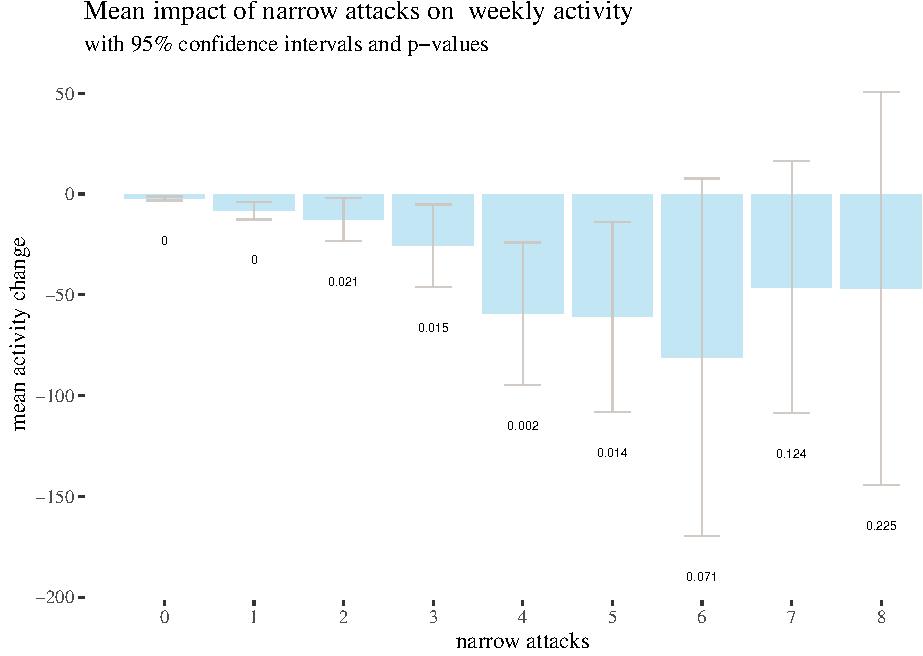
\includegraphics[width=1\linewidth]{redditAnalysisWalkthrough_files/figure-latex/unnamed-chunk-28-1} \end{center}
\end{subfigure}
\caption{T-test estimation of activity change by narrow attacks received. All available t-tests.}
\label{fig:highbar}
\end{figure}

\begin{figure}[h!]
\begin{subfigure}[t]{0.95\textwidth}

\begin{center}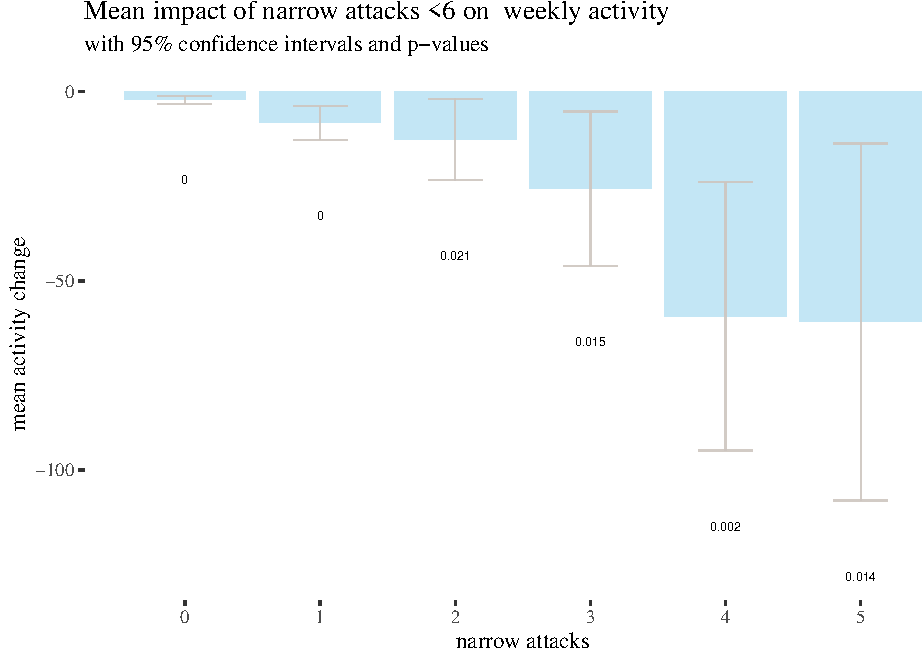
\includegraphics[width=1\linewidth]{redditAnalysisWalkthrough_files/figure-latex/unnamed-chunk-29-1} \end{center}
\end{subfigure}
\caption{T-test estimation of activity change by narrow attacks received (0-5).}
\label{fig:highbar6}
\end{figure}

\begin{figure}[h!]
\begin{subfigure}[t]{0.95\textwidth}

\begin{center}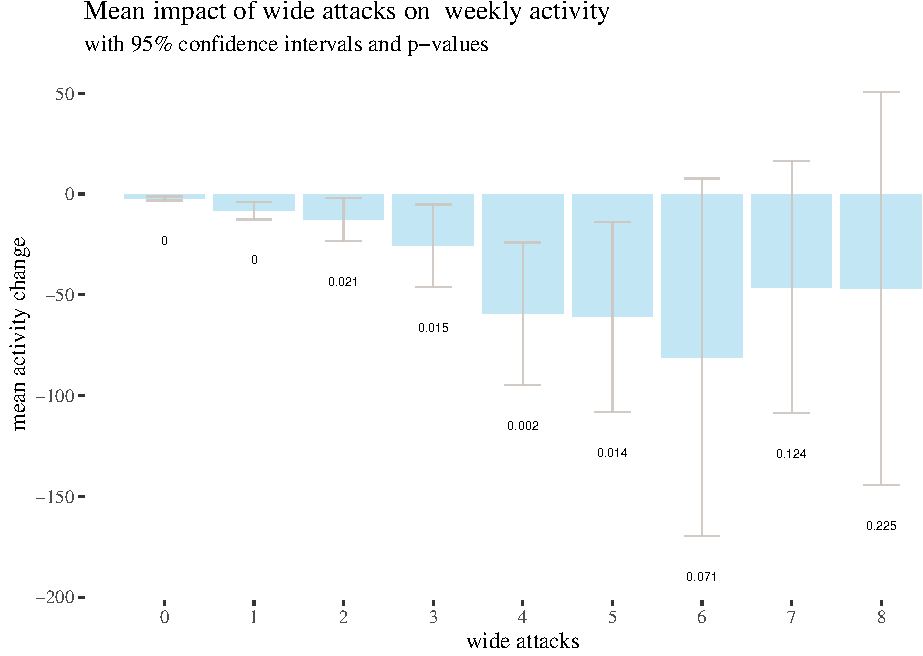
\includegraphics[width=1\linewidth]{redditAnalysisWalkthrough_files/figure-latex/unnamed-chunk-30-1} \end{center}
\end{subfigure}
\caption{T-test estimation of activity change by narrow attacks received (0-2).}
\label{fig:highbar3}
\end{figure}

\begin{figure}[h!]

\centering
\begin{subfigure}[t]{0.75\textwidth}

\begin{center}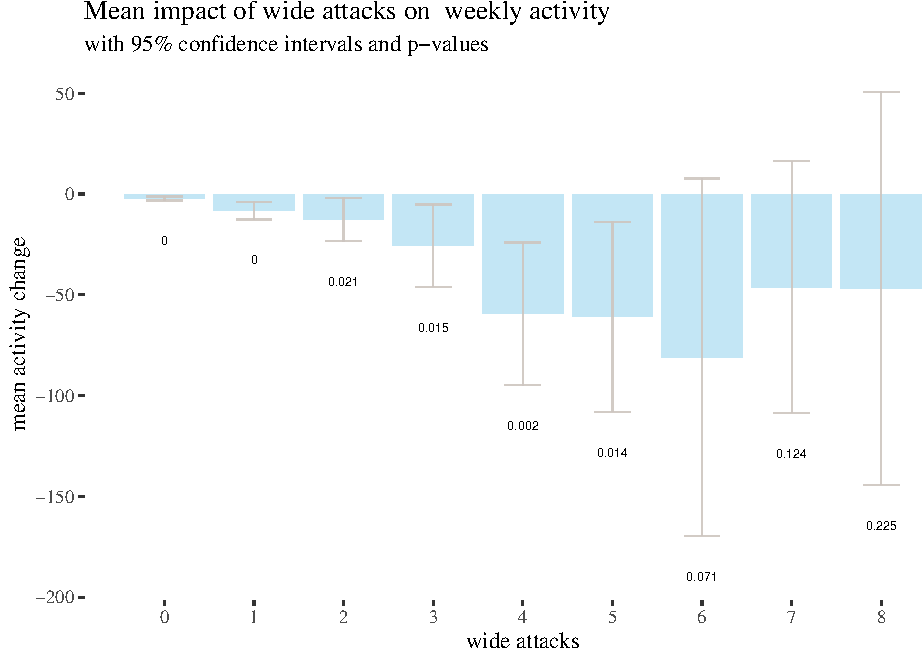
\includegraphics[width=1\linewidth]{redditAnalysisWalkthrough_files/figure-latex/unnamed-chunk-31-1} \end{center}
\caption{wide attacks.}
\end{subfigure}
 
\begin{subfigure}[t]{0.75\textwidth}

\begin{center}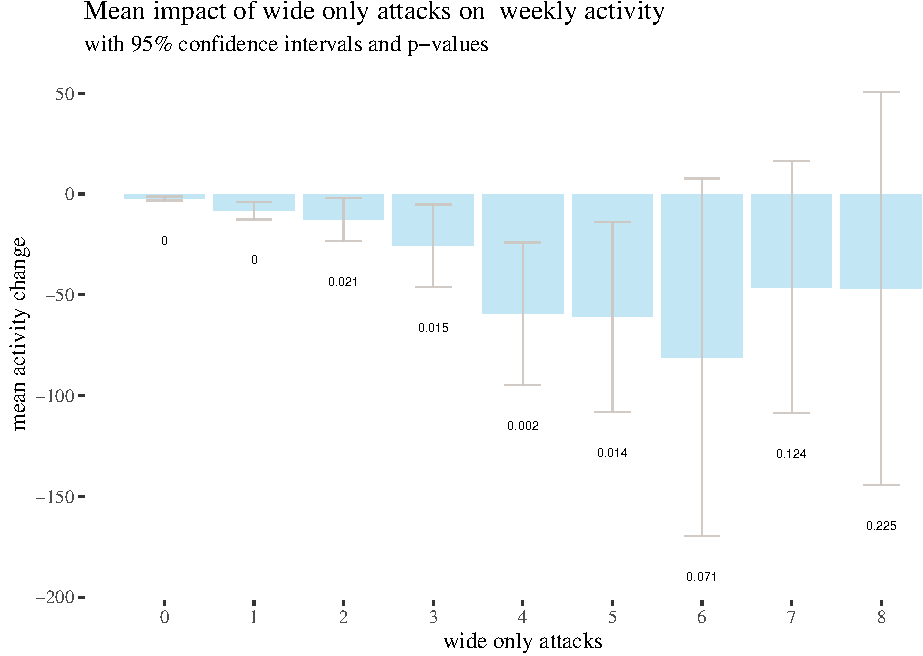
\includegraphics[width=1\linewidth]{redditAnalysisWalkthrough_files/figure-latex/unnamed-chunk-32-1} \end{center}
\caption{wide only attacks}
\end{subfigure}

\caption{Estimated means of activity change by the number of wide and wide only attacks, with 95\% confidence intervals and rounded $p$-values printed.}
\label{fig:lowerTableBars}
\end{figure}

\footnotesize

\begin{Shaded}
\begin{Highlighting}[]
\NormalTok{h6 <-}\StringTok{ }\NormalTok{data[data}\OperatorTok{$}\NormalTok{sumHighBefore }\OperatorTok{==}\StringTok{ }\DecValTok{6}\NormalTok{, ]}
\NormalTok{h7 <-}\StringTok{ }\NormalTok{data[data}\OperatorTok{$}\NormalTok{sumHighBefore }\OperatorTok{==}\StringTok{ }\DecValTok{7}\NormalTok{, ]}
\NormalTok{h8 <-}\StringTok{ }\NormalTok{data[data}\OperatorTok{$}\NormalTok{sumHighBefore }\OperatorTok{==}\StringTok{ }\DecValTok{8}\NormalTok{, ]}

\CommentTok{# power for 6 attacks}
\NormalTok{a <-}\StringTok{ }\KeywordTok{mean}\NormalTok{(data}\OperatorTok{$}\NormalTok{activityDiff)}
\NormalTok{s <-}\StringTok{ }\KeywordTok{sd}\NormalTok{(h7}\OperatorTok{$}\NormalTok{activityDiff)}
\NormalTok{n <-}\StringTok{ }\DecValTok{8}
\NormalTok{error <-}\StringTok{ }\KeywordTok{qt}\NormalTok{(}\FloatTok{0.975}\NormalTok{, }\DataTypeTok{df =}\NormalTok{ n }\OperatorTok{-}\StringTok{ }\DecValTok{1}\NormalTok{) }\OperatorTok{*}\StringTok{ }\NormalTok{s}\OperatorTok{/}\KeywordTok{sqrt}\NormalTok{(n)}
\NormalTok{left <-}\StringTok{ }\NormalTok{a }\OperatorTok{-}\StringTok{ }\NormalTok{error}
\NormalTok{right <-}\StringTok{ }\NormalTok{a }\OperatorTok{+}\StringTok{ }\NormalTok{error}
\NormalTok{assumed <-}\StringTok{ }\NormalTok{a }\OperatorTok{-}\StringTok{ }\DecValTok{80}
\NormalTok{tleft <-}\StringTok{ }\NormalTok{(left }\OperatorTok{-}\StringTok{ }\NormalTok{assumed)}\OperatorTok{/}\NormalTok{(s}\OperatorTok{/}\KeywordTok{sqrt}\NormalTok{(n))}
\NormalTok{tright <-}\StringTok{ }\NormalTok{(right }\OperatorTok{-}\StringTok{ }\NormalTok{assumed)}\OperatorTok{/}\NormalTok{(s}\OperatorTok{/}\KeywordTok{sqrt}\NormalTok{(n))}
\NormalTok{p <-}\StringTok{ }\KeywordTok{pt}\NormalTok{(tright, }\DataTypeTok{df =}\NormalTok{ n }\OperatorTok{-}\StringTok{ }\DecValTok{1}\NormalTok{) }\OperatorTok{-}\StringTok{ }\KeywordTok{pt}\NormalTok{(tleft, }\DataTypeTok{df =}\NormalTok{ n }\OperatorTok{-}\StringTok{ }\DecValTok{1}\NormalTok{)}
\NormalTok{power6 <-}\StringTok{ }\DecValTok{1} \OperatorTok{-}\StringTok{ }\NormalTok{p}

\CommentTok{# power for 7 attacks}
\NormalTok{a <-}\StringTok{ }\KeywordTok{mean}\NormalTok{(data}\OperatorTok{$}\NormalTok{activityDiff)}
\NormalTok{s <-}\StringTok{ }\KeywordTok{sd}\NormalTok{(h7}\OperatorTok{$}\NormalTok{activityDiff)}
\NormalTok{n <-}\StringTok{ }\DecValTok{8}
\NormalTok{error <-}\StringTok{ }\KeywordTok{qt}\NormalTok{(}\FloatTok{0.975}\NormalTok{, }\DataTypeTok{df =}\NormalTok{ n }\OperatorTok{-}\StringTok{ }\DecValTok{1}\NormalTok{) }\OperatorTok{*}\StringTok{ }\NormalTok{s}\OperatorTok{/}\KeywordTok{sqrt}\NormalTok{(n)}
\NormalTok{left <-}\StringTok{ }\NormalTok{a }\OperatorTok{-}\StringTok{ }\NormalTok{error}
\NormalTok{right <-}\StringTok{ }\NormalTok{a }\OperatorTok{+}\StringTok{ }\NormalTok{error}
\NormalTok{assumed <-}\StringTok{ }\NormalTok{a }\OperatorTok{-}\StringTok{ }\DecValTok{80}
\NormalTok{tleft <-}\StringTok{ }\NormalTok{(left }\OperatorTok{-}\StringTok{ }\NormalTok{assumed)}\OperatorTok{/}\NormalTok{(s}\OperatorTok{/}\KeywordTok{sqrt}\NormalTok{(n))}
\NormalTok{tright <-}\StringTok{ }\NormalTok{(right }\OperatorTok{-}\StringTok{ }\NormalTok{assumed)}\OperatorTok{/}\NormalTok{(s}\OperatorTok{/}\KeywordTok{sqrt}\NormalTok{(n))}
\NormalTok{p <-}\StringTok{ }\KeywordTok{pt}\NormalTok{(tright, }\DataTypeTok{df =}\NormalTok{ n }\OperatorTok{-}\StringTok{ }\DecValTok{1}\NormalTok{) }\OperatorTok{-}\StringTok{ }\KeywordTok{pt}\NormalTok{(tleft, }\DataTypeTok{df =}\NormalTok{ n }\OperatorTok{-}\StringTok{ }\DecValTok{1}\NormalTok{)}
\NormalTok{power7 <-}\StringTok{ }\DecValTok{1} \OperatorTok{-}\StringTok{ }\NormalTok{p}

\CommentTok{# power for 8 attacks}
\NormalTok{a <-}\StringTok{ }\KeywordTok{mean}\NormalTok{(data}\OperatorTok{$}\NormalTok{activityDiff)}
\NormalTok{s <-}\StringTok{ }\KeywordTok{sd}\NormalTok{(h8}\OperatorTok{$}\NormalTok{activityDiff)}
\NormalTok{n <-}\StringTok{ }\DecValTok{4}
\NormalTok{error <-}\StringTok{ }\KeywordTok{qt}\NormalTok{(}\FloatTok{0.975}\NormalTok{, }\DataTypeTok{df =}\NormalTok{ n }\OperatorTok{-}\StringTok{ }\DecValTok{1}\NormalTok{) }\OperatorTok{*}\StringTok{ }\NormalTok{s}\OperatorTok{/}\KeywordTok{sqrt}\NormalTok{(n)}
\NormalTok{left <-}\StringTok{ }\NormalTok{a }\OperatorTok{-}\StringTok{ }\NormalTok{error}
\NormalTok{right <-}\StringTok{ }\NormalTok{a }\OperatorTok{+}\StringTok{ }\NormalTok{error}
\NormalTok{assumed <-}\StringTok{ }\NormalTok{a }\OperatorTok{-}\StringTok{ }\DecValTok{80}
\NormalTok{tleft <-}\StringTok{ }\NormalTok{(left }\OperatorTok{-}\StringTok{ }\NormalTok{assumed)}\OperatorTok{/}\NormalTok{(s}\OperatorTok{/}\KeywordTok{sqrt}\NormalTok{(n))}
\NormalTok{tright <-}\StringTok{ }\NormalTok{(right }\OperatorTok{-}\StringTok{ }\NormalTok{assumed)}\OperatorTok{/}\NormalTok{(s}\OperatorTok{/}\KeywordTok{sqrt}\NormalTok{(n))}
\NormalTok{p <-}\StringTok{ }\KeywordTok{pt}\NormalTok{(tright, }\DataTypeTok{df =}\NormalTok{ n }\OperatorTok{-}\StringTok{ }\DecValTok{1}\NormalTok{) }\OperatorTok{-}\StringTok{ }\KeywordTok{pt}\NormalTok{(tleft, }\DataTypeTok{df =}\NormalTok{ n }\OperatorTok{-}\StringTok{ }\DecValTok{1}\NormalTok{)}
\NormalTok{power8 <-}\StringTok{ }\DecValTok{1} \OperatorTok{-}\StringTok{ }\NormalTok{p}
\end{Highlighting}
\end{Shaded}

\normalsize 

Note fairly wide confidence intervals for higher number of attacks.
These arise because attacks are quite rare, so the sample sizes for 5,
6, 7 and 8 narrow attacks are 22, 17, 8 and 4 respectively. This might
be also the reason why \(p\)-values are not too low (although still
below the usual significance thresholds). In fact, power analysis shows
that if the real activity difference for those groups equals to the mean
for \textsf{narrow = 6}, that is, -80, the probabilities that this
effect would be discovered by a single sample t-test for 6, 7, and 8
attacks are 0.737, 0.737, 0.309, and so tests for higher numbers of
attacks are underpowered.

We run single t-tests on different groups to estimate different means
and we don't use t-test for hypothesis testing. To alleviate concerns
about multiple testing and increased risk of type I error, we also
performed an ANOVA tests, which strongly suggest non-random correlation
between the numbers of attacks and activity change. Furthermore, 80
comparison rows in Tukey's Honest Significance Test (Tukey, 1949) have
conservatively adjusted p-value below 0.05.

\footnotesize

\begin{Shaded}
\begin{Highlighting}[]
\NormalTok{highAnova <-}\StringTok{ }\KeywordTok{aov}\NormalTok{(activityDiff }\OperatorTok{~}\StringTok{ }\KeywordTok{as.factor}\NormalTok{(sumHighBefore), }\DataTypeTok{data =}\NormalTok{ data)}
\NormalTok{lowAnova <-}\StringTok{ }\KeywordTok{aov}\NormalTok{(activityDiff }\OperatorTok{~}\StringTok{ }\KeywordTok{as.factor}\NormalTok{(sumLowBefore), }\DataTypeTok{data =}\NormalTok{ data)}
\NormalTok{lowOnlyAnova <-}\StringTok{ }\KeywordTok{aov}\NormalTok{(activityDiff }\OperatorTok{~}\StringTok{ }\KeywordTok{as.factor}\NormalTok{(sumLowBefore }\OperatorTok{-}\StringTok{ }\NormalTok{sumHighBefore),}
    \DataTypeTok{data =}\NormalTok{ data)}

\KeywordTok{library}\NormalTok{(descr, }\DataTypeTok{quietly =} \OtherTok{TRUE}\NormalTok{)}
\KeywordTok{library}\NormalTok{(pander, }\DataTypeTok{quietly =} \OtherTok{TRUE}\NormalTok{)}
\KeywordTok{library}\NormalTok{(papeR, }\DataTypeTok{quietly =} \OtherTok{TRUE}\NormalTok{)}
\NormalTok{sh <-}\StringTok{ }\KeywordTok{xtable}\NormalTok{(}\KeywordTok{summary}\NormalTok{(highAnova))}
\KeywordTok{rownames}\NormalTok{(sh) <-}\StringTok{ }\KeywordTok{c}\NormalTok{(}\StringTok{"narrow"}\NormalTok{, }\StringTok{"residuals"}\NormalTok{)}
\NormalTok{sh}
\end{Highlighting}
\end{Shaded}

\normalsize

\begin{table}[h!]

\begin{tabular}{l|r|r|r|r|r}
\hline
  & Df & Sum Sq & Mean Sq & F value & Pr(>F)\\
\hline
narrow & 20 & 785496 & 39274.798 & 25.03076 & 0\\
\hline
residuals & 3652 & 5730212 & 1569.061 &  & \\
\hline
\end{tabular}
\caption{ANOVA for activity change vs. narrow attacks received.}
\label{tab:anovanarrow}
\end{table}

\begin{table}[h!]

\begin{tabular}{l|r|r|r|r|r}
\hline
  & Df & Sum Sq & Mean Sq & F value & Pr(>F)\\
\hline
narrow & 42 & 1103366 & 26270.608 & 17.61941 & 0\\
\hline
residuals & 3630 & 5412343 & 1491.004 &  & \\
\hline
\end{tabular}
\caption{ANOVA for activity change vs. wide attacks received.}
\label{tab:anovawide}
\end{table}

\begin{table}[h!]

\begin{tabular}{l|r|r|r|r|r}
\hline
  & Df & Sum Sq & Mean Sq & F value & Pr(>F)\\
\hline
narrow & 35 & 1106625 & 31617.869 & 21.25946 & 0\\
\hline
residuals & 3637 & 5409083 & 1487.238 &  & \\
\hline
\end{tabular}
\caption{ANOVA for activity change vs. wide only attacks received.}
\label{tab:anovawideonly}
\end{table}

We used t-tests, which one might think assumes normality, to estimate
means for distributions, which in fact are not normal. However, what
t-test assumes is the normality of the sampling distribution, and this
condition is much easier to satisfy thanks to the central limit theorem.
(see for instance Figure \ref{fig:sampling}).\}

\footnotesize

\begin{Shaded}
\begin{Highlighting}[]
\NormalTok{means <-}\StringTok{ }\KeywordTok{numeric}\NormalTok{(}\DecValTok{10000}\NormalTok{)}
\ControlFlowTok{for}\NormalTok{ (run }\ControlFlowTok{in} \DecValTok{1}\OperatorTok{:}\DecValTok{10000}\NormalTok{) \{}
\NormalTok{    means[run] <-}\StringTok{ }\KeywordTok{mean}\NormalTok{(}\KeywordTok{sample}\NormalTok{(data[data}\OperatorTok{$}\NormalTok{sumHighBefore }\OperatorTok{==}\StringTok{ }\DecValTok{2}\NormalTok{, ]}\OperatorTok{$}\NormalTok{activityDiff,}
        \DecValTok{30}\NormalTok{))}
\NormalTok{\}}
\NormalTok{distr <-}\StringTok{ }\KeywordTok{ggplot}\NormalTok{(data[data}\OperatorTok{$}\NormalTok{sumHighBefore }\OperatorTok{==}\StringTok{ }\DecValTok{2}\NormalTok{, ], }\KeywordTok{aes}\NormalTok{(}\DataTypeTok{x =}\NormalTok{ activityDiff)) }\OperatorTok{+}
\StringTok{    }\KeywordTok{geom_histogram}\NormalTok{(}\DataTypeTok{bins =} \DecValTok{100}\NormalTok{) }\OperatorTok{+}\StringTok{ }\NormalTok{th }\OperatorTok{+}\StringTok{ }\KeywordTok{ggtitle}\NormalTok{(}\StringTok{"Distribution of activityDiff for narrow attacks before = 2"}\NormalTok{)}


\NormalTok{sampDistr <-}\StringTok{ }\KeywordTok{ggplot}\NormalTok{() }\OperatorTok{+}\StringTok{ }\KeywordTok{geom_histogram}\NormalTok{(}\KeywordTok{aes}\NormalTok{(}\DataTypeTok{x =}\NormalTok{ means), }\DataTypeTok{bins =} \DecValTok{100}\NormalTok{) }\OperatorTok{+}
\StringTok{    }\NormalTok{th }\OperatorTok{+}\StringTok{ }\KeywordTok{ggtitle}\NormalTok{(}\StringTok{"Simulated sampling distribution for the same  with n=30 and 10 000 runs"}\NormalTok{)}
\end{Highlighting}
\end{Shaded}

\normalsize

\begin{figure}
\begin{subfigure}{0.4\textwidth}

\begin{center}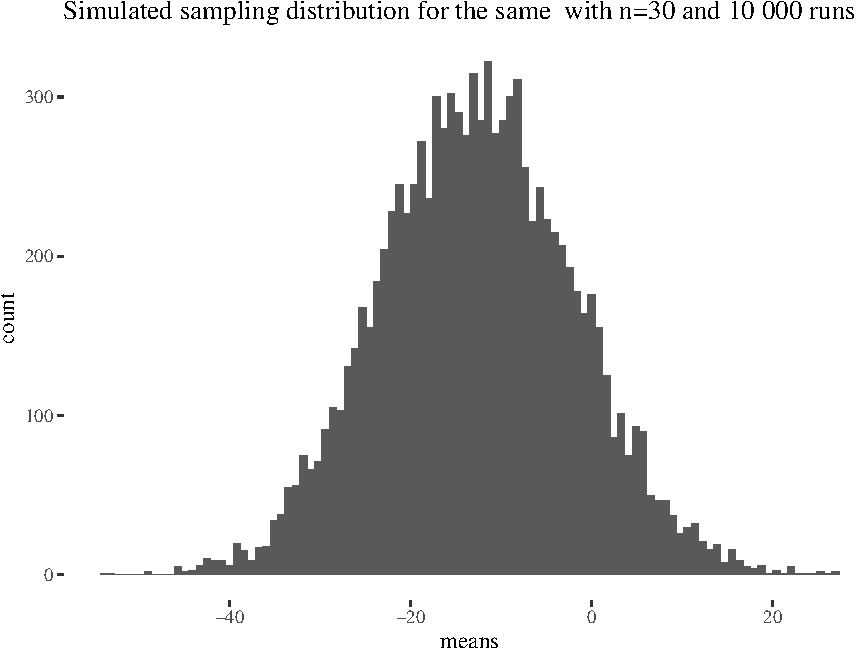
\includegraphics{redditAnalysisWalkthrough_files/figure-latex/unnamed-chunk-39-1} \end{center}
\end{subfigure}\hfill
\begin{subfigure}{0.4\textwidth}

\begin{center}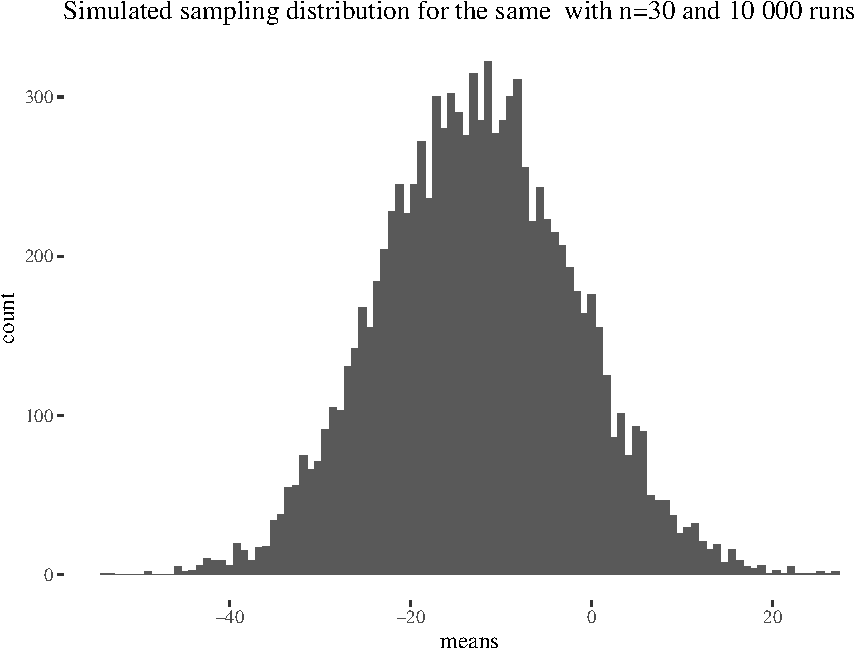
\includegraphics{redditAnalysisWalkthrough_files/figure-latex/unnamed-chunk-40-1} \end{center}
\end{subfigure}
\caption{Example of comparison of a distribution and its sampling distribution.}
\label{fig:sampling}
\end{figure}

There are, however, some reasons to be concerned with classical methods:

\begin{itemize}
\item
  \(p\)-values and confidence intervals are hard to interpret
  intuitively. For instance, a 95\% confidence interval being \((x,y)\)
  does not mean that the true mean is within \((x,y)\) with probability
  \(0.95\), and the estimated mean being \(z\) with \(p\)-value \(0.01\)
  does not mean that the true population mean is \(z\) with probability
  \(0.99\).
\item
  \(p\)-values and confidence intervals are sensitive to undesirable
  factors, such as stopping intention in experiment design (Kruschke,
  2015).
\item
  Classical hypothesis tests require several assumptions to hold which
  sometimes do not hold in reality, and the choice of significance
  thresholds is arbitrary.
\item
  Crucially, probabilities reported in classical analysis are
  probabilities of the data on the assumption of the null hypothesis
  (e.g., that the true mean is 0), not the posterior probabilities of
  the true parameter values given the data. To obtain these, we used
  Bayesian analysis and studied the impact of skeptical prior
  probabilities on how the data impacts the posterior distribution of
  the parameters at hand.
\end{itemize}

\section{Bayesian estimation}

We used Markov Chain Monte Carlo methods (using the
\textsf{Bayesian Estimation Supersedes the t-Test}\footnote{\url{https://www.rdocumentation.org/packages/BEST/versions/0.5.2}}
package) to estimate the posterior probability distribution for mean
changes in activity in different groups We did this for three different
fairly skeptical normal prior distributions (which we call
\textsf{wide, informed}, and \textsf{fit}), whose means and standard
deviations are respectively \((0,50), (-1.11,44.47)\) and
\((-1.11,7.5)\) (read on for an explanation why).

\footnotesize

\begin{Shaded}
\begin{Highlighting}[]
\KeywordTok{library}\NormalTok{(BEST)}
\NormalTok{priorsWide <-}\StringTok{ }\KeywordTok{list}\NormalTok{(}\DataTypeTok{muM =} \DecValTok{0}\NormalTok{, }\DataTypeTok{muSD =} \DecValTok{50}\NormalTok{)}
\NormalTok{priorsInformed <-}\StringTok{ }\KeywordTok{list}\NormalTok{(}\DataTypeTok{muM =} \FloatTok{-1.11}\NormalTok{, }\DataTypeTok{muSD =} \FloatTok{44.47}\NormalTok{)}
\NormalTok{priorsFit <-}\StringTok{ }\KeywordTok{list}\NormalTok{(}\DataTypeTok{muM =} \FloatTok{-1.11}\NormalTok{, }\DataTypeTok{muSD =} \FloatTok{7.5}\NormalTok{)}
\end{Highlighting}
\end{Shaded}

\normalsize

These are all normal distributions with different parameters. We follow
the usual practice of presenting a Bayesian analysis with a range of
options: the reader is to judge with prior seems most plausible to them,
and then modify their beliefs according to the impact the data has on
their prior convictions. The wide prior assumes that the most likely
difference is 0, but the standard deviation is quite large, the informed
prior takes the mean and standard deviation of the whole study group,
whereas the fit prior follows fairly closely the actual empirical
distribution of activity change values. All of them are fairly skeptical
because they expect the change to be the same for every user, and they
expect this change to be near 0. We did not use a completely uninformed
uniform prior, because it is not sufficiently skeptical, being more
easily impacted by the data, and because it has some undesirable
mathematical
properties\footnote{See \emph{Don’t Use Uniform Priors. They statistically don’t make sense.} at \url{https://towardsdatascience.com/stop-using-uniform-priors-47473bdd0b8a} for an accessible explanation.}
Our priors look as in Figure \ref{fig:priors} (note that the fitted
prior looks similar when the \(x\) scale is different to make the
fitting more clearly visible; we also visualise the fitted prior in the
same scale as the other priors). Here's the visualisation code for the
wide priors, code for the other priors is analogous.

\footnotesize

\begin{Shaded}
\begin{Highlighting}[]
\NormalTok{priorWide <-}\StringTok{ }\KeywordTok{ggplot}\NormalTok{(}\DataTypeTok{data =} \KeywordTok{data.frame}\NormalTok{(}\DataTypeTok{x =} \KeywordTok{c}\NormalTok{(}\OperatorTok{-}\DecValTok{200}\NormalTok{, }\DecValTok{200}\NormalTok{)), }\KeywordTok{aes}\NormalTok{(x)) }\OperatorTok{+}
\StringTok{    }\KeywordTok{stat_function}\NormalTok{(}\DataTypeTok{fun =}\NormalTok{ dnorm, }\DataTypeTok{args =} \KeywordTok{list}\NormalTok{(}\DataTypeTok{mean =} \DecValTok{0}\NormalTok{, }\DataTypeTok{sd =} \DecValTok{50}\NormalTok{)) }\OperatorTok{+}
\StringTok{    }\KeywordTok{ylab}\NormalTok{(}\StringTok{""}\NormalTok{) }\OperatorTok{+}\StringTok{ }\KeywordTok{scale_y_continuous}\NormalTok{(}\DataTypeTok{breaks =} \OtherTok{NULL}\NormalTok{) }\OperatorTok{+}\StringTok{ }\NormalTok{th }\OperatorTok{+}\StringTok{ }\KeywordTok{xlab}\NormalTok{(}\StringTok{"expected activity change"}\NormalTok{) }\OperatorTok{+}
\StringTok{    }\KeywordTok{labs}\NormalTok{(}\DataTypeTok{title =} \StringTok{"Wide prior"}\NormalTok{, }\DataTypeTok{subtitle =} \StringTok{"Normal prior with m = 0, sd = 50"}\NormalTok{)}
\NormalTok{priorWide}
\end{Highlighting}
\end{Shaded}

\normalsize

\begin{figure}[!ht]
\begin{subfigure}[!ht]{0.45\textwidth}

\begin{center}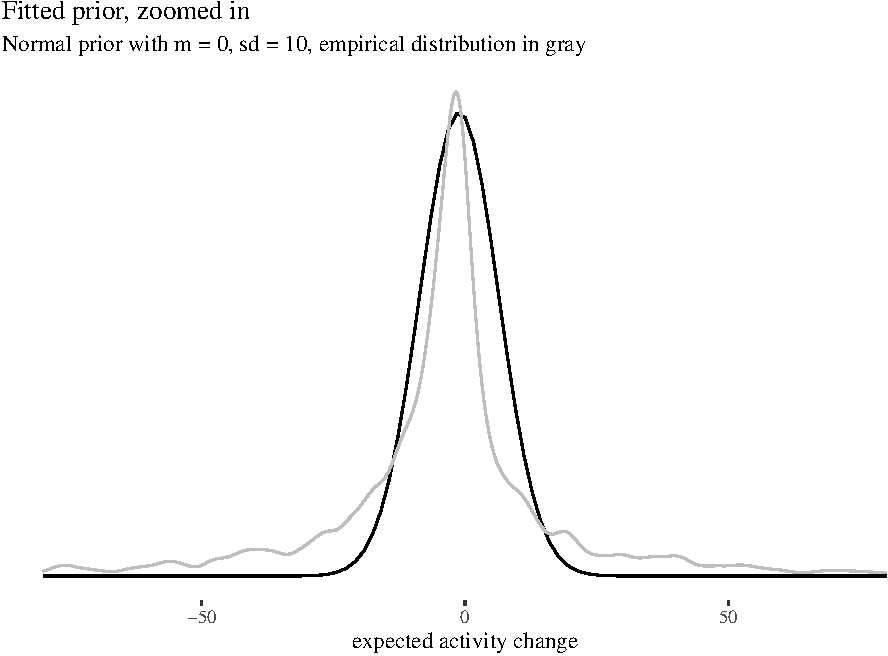
\includegraphics[width=1\linewidth]{redditAnalysisWalkthrough_files/figure-latex/unnamed-chunk-43-1} \end{center}
\end{subfigure}
\hfill
\begin{subfigure}[!ht]{0.45\textwidth}

\begin{center}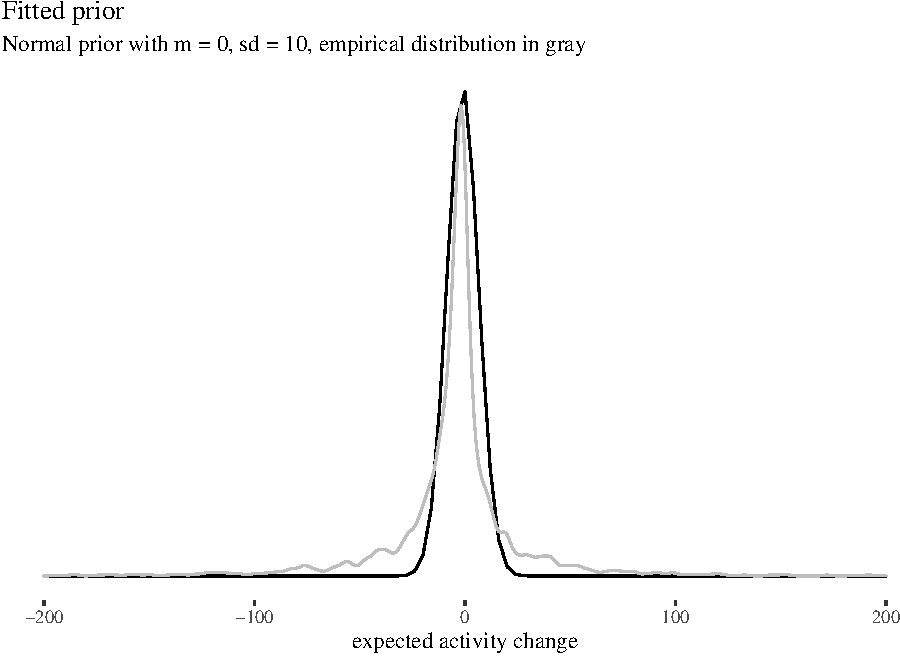
\includegraphics[width=1\linewidth]{redditAnalysisWalkthrough_files/figure-latex/unnamed-chunk-44-1} \end{center}
\end{subfigure}




\begin{subfigure}[!ht]{0.45\textwidth}

\begin{center}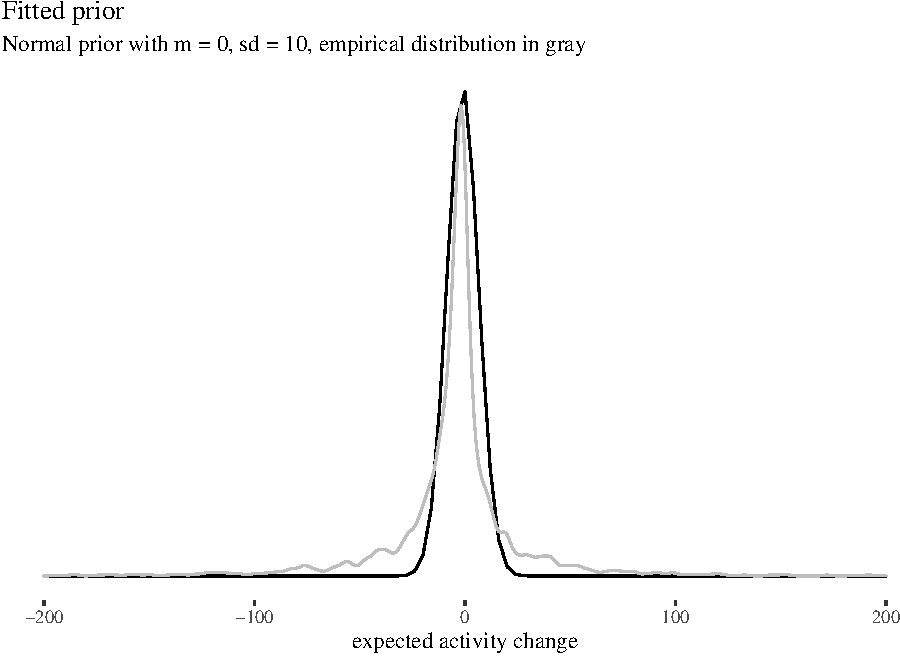
\includegraphics[width=1\linewidth]{redditAnalysisWalkthrough_files/figure-latex/unnamed-chunk-45-1} \end{center}
\end{subfigure} \hfill
\begin{subfigure}[!ht]{0.45\textwidth}

\begin{center}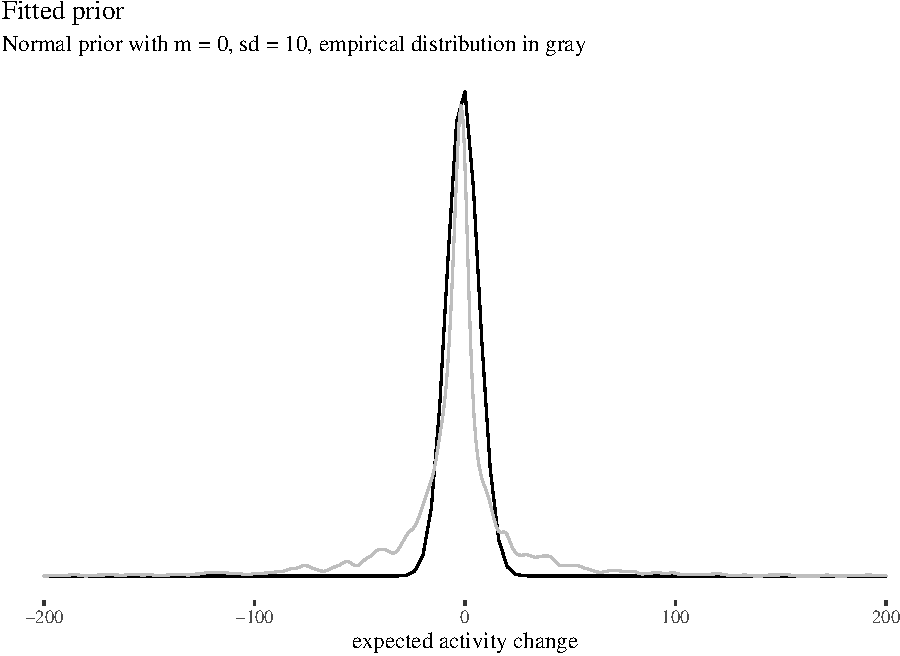
\includegraphics[width=1\linewidth]{redditAnalysisWalkthrough_files/figure-latex/unnamed-chunk-46-1} \end{center}
\end{subfigure}


\caption{Wide and two informative skeptical priors for our Bayesian analysis.}
\label{fig:priors}
\end{figure}

First, it will be convenient to split and extract the data (we will do
the Bayesian analysis for narrow attacks:

\footnotesize

\begin{Shaded}
\begin{Highlighting}[]
\NormalTok{sh0 <-}\StringTok{ }\NormalTok{data[data}\OperatorTok{$}\NormalTok{sumHighBefore }\OperatorTok{==}\StringTok{ }\DecValTok{0}\NormalTok{, ]}\OperatorTok{$}\NormalTok{activityDiff}
\NormalTok{sh1 <-}\StringTok{ }\NormalTok{data[data}\OperatorTok{$}\NormalTok{sumHighBefore }\OperatorTok{==}\StringTok{ }\DecValTok{1}\NormalTok{, ]}\OperatorTok{$}\NormalTok{activityDiff}
\NormalTok{sh2 <-}\StringTok{ }\NormalTok{data[data}\OperatorTok{$}\NormalTok{sumHighBefore }\OperatorTok{==}\StringTok{ }\DecValTok{2}\NormalTok{, ]}\OperatorTok{$}\NormalTok{activityDiff}
\NormalTok{sh3 <-}\StringTok{ }\NormalTok{data[data}\OperatorTok{$}\NormalTok{sumHighBefore }\OperatorTok{==}\StringTok{ }\DecValTok{3}\NormalTok{, ]}\OperatorTok{$}\NormalTok{activityDiff}
\NormalTok{sh4 <-}\StringTok{ }\NormalTok{data[data}\OperatorTok{$}\NormalTok{sumHighBefore }\OperatorTok{==}\StringTok{ }\DecValTok{4}\NormalTok{, ]}\OperatorTok{$}\NormalTok{activityDiff}
\NormalTok{sh5 <-}\StringTok{ }\NormalTok{data[data}\OperatorTok{$}\NormalTok{sumHighBefore }\OperatorTok{==}\StringTok{ }\DecValTok{5}\NormalTok{, ]}\OperatorTok{$}\NormalTok{activityDiff}
\NormalTok{sh6 <-}\StringTok{ }\NormalTok{data[data}\OperatorTok{$}\NormalTok{sumHighBefore }\OperatorTok{==}\StringTok{ }\DecValTok{6}\NormalTok{, ]}\OperatorTok{$}\NormalTok{activityDiff}
\NormalTok{sh7 <-}\StringTok{ }\NormalTok{data[data}\OperatorTok{$}\NormalTok{sumHighBefore }\OperatorTok{==}\StringTok{ }\DecValTok{7}\NormalTok{, ]}\OperatorTok{$}\NormalTok{activityDiff}
\NormalTok{sh8 <-}\StringTok{ }\NormalTok{data[data}\OperatorTok{$}\NormalTok{sumHighBefore }\OperatorTok{==}\StringTok{ }\DecValTok{8}\NormalTok{, ]}\OperatorTok{$}\NormalTok{activityDiff}
\end{Highlighting}
\end{Shaded}

\normalsize

As an example, we go over in detail over the estimation of the impact of
data for three narrow attacks on the wide prior. We built the sample of
simulated posterior probabilities and plotted the t-distributions of 30
random steps in the approximation process together with a histogram of
the data, so that we can estimate how the simulations
converged.\footnote{Actually, since BEST simulations are computationally heavy, we have already run them separately and loaded the file with the results. However, normally you would use a line like the one listed (these simulations take the more time the larger the dataset).}

\footnotesize

\begin{Shaded}
\begin{Highlighting}[]
\NormalTok{mc3w <-}\StringTok{ }\KeywordTok{BESTmcmc}\NormalTok{(sh3, }\DataTypeTok{priors =}\NormalTok{ priorsWide)}
\KeywordTok{plotPostPred}\NormalTok{(mc3w)}
\end{Highlighting}
\end{Shaded}

\normalsize

\begin{figure}

\begin{center}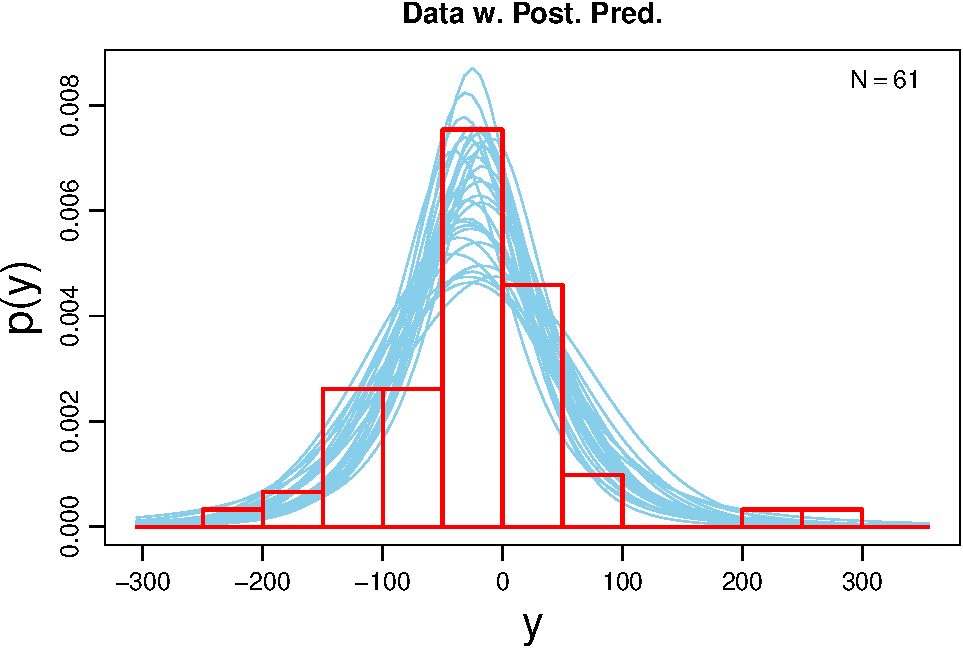
\includegraphics[width=1\linewidth]{redditAnalysisWalkthrough_files/figure-latex/unnamed-chunk-50-1} \end{center}
\label{fig:threeWidePostPred}
\caption{T-distributions for 30 random steps in Bayesian approximation (wide prior, three attacks): $y$ is a potential parameter value (a candidate group mean), and we plot probability densities for the distributions detemined by the random steps.}
\end{figure}

Next, we print some information about the object we obtained:

\footnotesize

\begin{Shaded}
\begin{Highlighting}[]
\KeywordTok{print}\NormalTok{(mc3w)}
\end{Highlighting}
\end{Shaded}

\begin{verbatim}
## MCMC fit results for BEST analysis:
## 100002 simulations saved.
##          mean     sd  median    HDIlo  HDIup  Rhat n.eff
## mu    -24.476  9.063 -24.327 -42.4760 -6.859 1.000 48767
## nu      9.626 12.988   5.275   0.9163 33.326 1.001  2867
## sigma  61.398 11.533  61.081  39.6685 84.249 1.000  9530
## 
## 'HDIlo' and 'HDIup' are the limits of a 95% HDI credible interval.
## 'Rhat' is the potential scale reduction factor (at convergence, Rhat=1).
## 'n.eff' is a crude measure of effective sample size.
\end{verbatim}

\normalsize

The simulation, among other things, produces out a sample of 100002
simulated posterior distributions of the mean, \textsf{mu}. Below we
briefly describe how the algorithm works.\\

\begin{itemize}
\item Potential parameter  candidates are "locations"  that can be visited, and as the algorithm "travels", it writes down the  visited ones.
\item The algorithm starts with a random candidate $\theta_1$ for a parameter, say, that the real mean activity change is 5. It writes down $\theta_1$ in the list of "places visited".
\item It calculates the probability (density) for the observations  on the assumption that $\theta_1$ indeed is the real mean activity change. This results in $p(D\vert \theta_1)$.
\item  However, what is important is $p(\theta_1\vert D)$, the extent to which the data supports the claim that $\theta_1$ is the right parameter. This, by Bayes' Theorem, is related to $p(D\vert \theta_1)$ by means of equation \eqref{eq:bayes}:
\begin{align}\label{eq:bayes}
p(\theta_1\vert D) & = \frac{p(D\vert \theta_1)p(\theta)}{p(D)}
\end{align}
\item Now, $p(D)$ is notoriously difficult to calculate in many cases.\footnote{The general problem is that  for the continuous case we have $p(D) = \int d \theta p(D\vert \theta) p (\theta)$ and this integral can be analytically unsolvable.}
However,  what the simulation needs is something proportional to the right-hand side above, and so what is used is simply $p(D\vert \theta_1)p(\theta)$: the likelihood times the prior. We call the result $p'(\theta_1)$.
\item Next, the algorithm considers another randomly drawn potential parameter $\theta_2$ in the neighborhood of $\theta_1$ and calculates $p'(\theta_2)$. If it is greater than $p'(\theta_1)$, it moves its location to $\theta_2$ with certainty, otherwise, it decides to move there with some non-extreme probability only (its value is a meta-parameter chosen to optimize the algorithm convergence).
\item Then it draws randomly another potential parameter in the neighborhood of wherever it ended up, and proceeds as before. This is done for a large number of steps. 
\item The procedure, repeated multiple  times, yields a long list of potential parameters visited, and the frequency with which the algorithm visits certain range of potential parameters is proportionate to the probability of these parameters being the true parameters given the data. After normalization,  a probability density for the list is obtained: this is the estimated posterior probability distribution  for the parameter in question.
\end{itemize}

For instance, it is possible to look at which potential parameters the
simulation for three attacks visited. Figure \ref{fig:chains} represents
the first 100 steps in the full simulation and parameters visited at
every 50th step (because a plot of all 100000 steps would not be clearly
readable).

\footnotesize

\begin{Shaded}
\begin{Highlighting}[]
\KeywordTok{ggplot}\NormalTok{() }\OperatorTok{+}\StringTok{ }\KeywordTok{geom_line}\NormalTok{(}\KeywordTok{aes}\NormalTok{(}\DataTypeTok{x =} \DecValTok{1}\OperatorTok{:}\KeywordTok{length}\NormalTok{(mc3w}\OperatorTok{$}\NormalTok{mu[}\DecValTok{1}\OperatorTok{:}\DecValTok{100}\NormalTok{]), }\DataTypeTok{y =}\NormalTok{ mc3w}\OperatorTok{$}\NormalTok{mu[}\DecValTok{1}\OperatorTok{:}\DecValTok{100}\NormalTok{]),}
    \DataTypeTok{alpha =} \FloatTok{0.7}\NormalTok{) }\OperatorTok{+}\StringTok{ }\NormalTok{th }\OperatorTok{+}\StringTok{ }\KeywordTok{xlab}\NormalTok{(}\StringTok{"initial steps in the chain"}\NormalTok{) }\OperatorTok{+}
\StringTok{    }\KeywordTok{ylab}\NormalTok{(}\StringTok{"potential parameter"}\NormalTok{) }\OperatorTok{+}\StringTok{ }\KeywordTok{labs}\NormalTok{(}\DataTypeTok{title =} \StringTok{"Convergence plot for first 100 steps in MCMC"}\NormalTok{,}
    \DataTypeTok{subtitle =} \StringTok{"Wide prior, three attacks"}\NormalTok{)}
\end{Highlighting}
\end{Shaded}

\normalsize

\begin{figure}[!ht]
\begin{subfigure}[!ht]{0.45\textwidth}

\begin{center}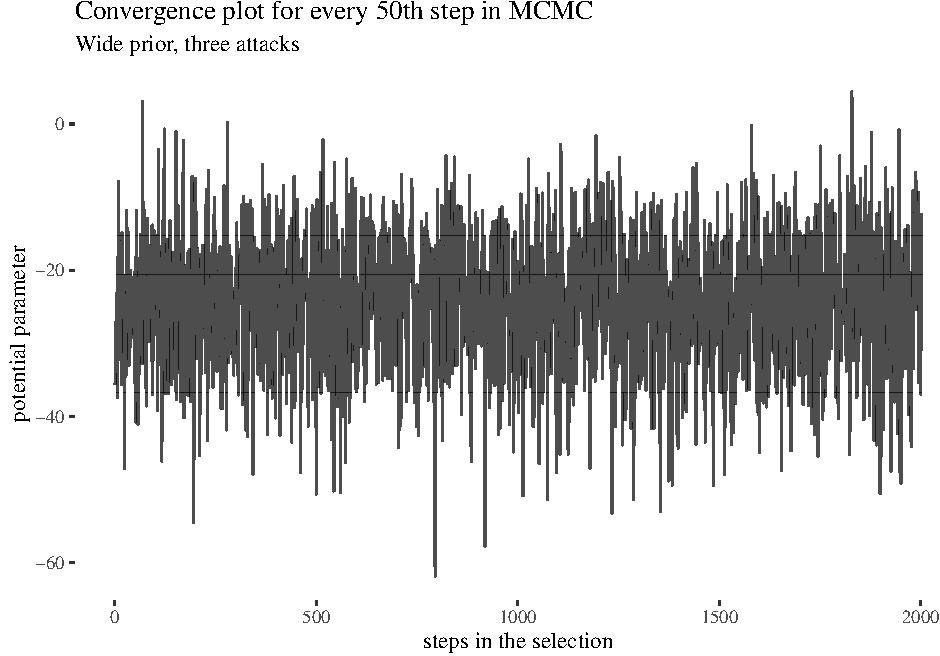
\includegraphics[width=1\linewidth]{redditAnalysisWalkthrough_files/figure-latex/unnamed-chunk-53-1} \end{center}
\end{subfigure} \hfill
\begin{subfigure}[!ht]{0.45\textwidth}

\begin{center}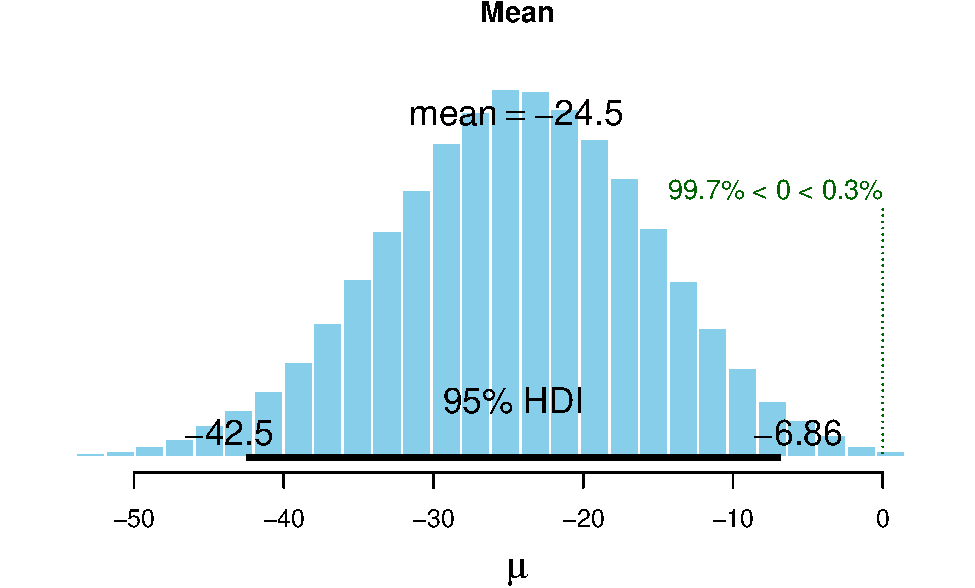
\includegraphics[width=1\linewidth]{redditAnalysisWalkthrough_files/figure-latex/unnamed-chunk-54-1} \end{center}
\end{subfigure}
\caption{Chain diagnostics for three attacks with wide priors.}
\label{fig:chains}
\end{figure}

We can collapse the plot, ignoring time, with default \textsf{BESTmcmc}
features and obtain Figure \ref{fig:mw3plot}. The histogram illustrates
the distribution of the outcome. HDI with limits is displayed at the
bottom, and the information in green represents the t proportion of the
sample that is below 0.

Rhat is a convergence measure, if the process goes well it should be
around 1, and \textsf{n.eff} is the effective sample size -- which is
often lower than the actual full sample because of autocorrelation (in
simulations next guess for a parameter depends to some extent on what
the previous guess was, and the calculation of \textsf{n.eff} corrects
for this).

\begin{figure}[h!]

\begin{center}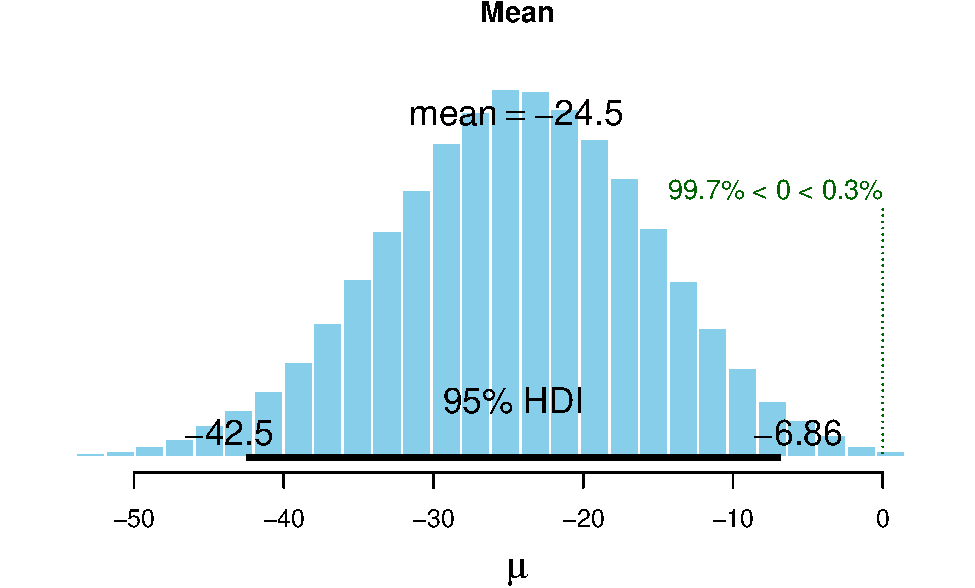
\includegraphics[width=1\linewidth]{redditAnalysisWalkthrough_files/figure-latex/unnamed-chunk-55-1} \end{center}
\caption{Outcome plot for three attacks, wide prior.}
\label{fig:mw3plot}
\end{figure}

Visual inspection of Figure \ref{fig:mw3plot} reveals that the most
visited locations (potential mean activity drops) center around slightly
less than minus twenty. In fact, the mean of those visited potential
means is -24.476 (although this does not have to be the mean of the
sample, which in our case is -25.6065574; rather it is the result of a
compromise between the data and the prior). The median is very close.
The new elements are HDIlo and HDIup, the limits of the
\emph{Highest Density Inverval}: the range of values that are most
credible and cover 95\% of the distribution. The Values within the 95\%
HDI are more credible than values outside the HDI, and the values inside
it have a total probability of 95\%. Crucially, these can be interpreted
as posterior probabilities of various mean candidates being the
population means based on the data, which makes HDI much unlike standard
confidence intervals.

Having gone over a detailed example, we present the results of the
Bayesian analysis for 0-9 narrow attacks (and a simulated prior) for
three types of priors and the barplot of the means of posterior
distributions (not the means of the data, but a result of a compromise
between the priors and the data) with HDIs. The total output is in
Figures \ref{fig:bayesian1}-\ref{fig:bayesian3}.

\footnotesize

\begin{Shaded}
\begin{Highlighting}[]
\CommentTok{# prepare data and plot densities}
\NormalTok{bayesianWideDF <-}\StringTok{ }\KeywordTok{data.frame}\NormalTok{(}\DataTypeTok{a0 =}\NormalTok{ mc0w}\OperatorTok{$}\NormalTok{mu, }\DataTypeTok{a1 =}\NormalTok{ mc1w}\OperatorTok{$}\NormalTok{mu, }\DataTypeTok{a2 =}\NormalTok{ mc2w}\OperatorTok{$}\NormalTok{mu,}
    \DataTypeTok{a3 =}\NormalTok{ mc3w}\OperatorTok{$}\NormalTok{mu, }\DataTypeTok{a4 =}\NormalTok{ mc4w}\OperatorTok{$}\NormalTok{mu, }\DataTypeTok{a5 =}\NormalTok{ mc5w}\OperatorTok{$}\NormalTok{mu, }\DataTypeTok{a6 =}\NormalTok{ mc6w}\OperatorTok{$}\NormalTok{mu, }\DataTypeTok{a7 =}\NormalTok{ mc7w}\OperatorTok{$}\NormalTok{mu,}
    \DataTypeTok{a8 =}\NormalTok{ mc8w}\OperatorTok{$}\NormalTok{mu)}
\NormalTok{bayesianWideDF}\OperatorTok{$}\NormalTok{prior <-}\StringTok{ }\KeywordTok{rnorm}\NormalTok{(}\KeywordTok{nrow}\NormalTok{(bayesianWideDF), }\DataTypeTok{mean =} \DecValTok{0}\NormalTok{,}
    \DataTypeTok{sd =} \DecValTok{50}\NormalTok{)}
\NormalTok{BayesianWideDFLong <-}\StringTok{ }\KeywordTok{gather}\NormalTok{(bayesianWideDF)}
\NormalTok{BayesianWideDFLong}\OperatorTok{$}\NormalTok{key <-}\StringTok{ }\KeywordTok{as.factor}\NormalTok{(BayesianWideDFLong}\OperatorTok{$}\NormalTok{key)}
\NormalTok{BayesianWideDensities <-}\StringTok{ }\KeywordTok{ggplot}\NormalTok{(BayesianWideDFLong, }\KeywordTok{aes}\NormalTok{(}\DataTypeTok{x =}\NormalTok{ value,}
    \DataTypeTok{group =}\NormalTok{ key, }\DataTypeTok{color =}\NormalTok{ key, }\DataTypeTok{fill =}\NormalTok{ key)) }\OperatorTok{+}\StringTok{ }\KeywordTok{geom_density}\NormalTok{(}\DataTypeTok{alpha =} \FloatTok{0.2}\NormalTok{) }\OperatorTok{+}
\StringTok{    }\NormalTok{th }\OperatorTok{+}\StringTok{ }\KeywordTok{xlab}\NormalTok{(}\StringTok{"activity change"}\NormalTok{) }\OperatorTok{+}\StringTok{ }\KeywordTok{scale_fill_discrete}\NormalTok{(}\DataTypeTok{name =} \StringTok{"group"}\NormalTok{,}
    \DataTypeTok{labels =} \KeywordTok{c}\NormalTok{(}\StringTok{"0 attacks"}\NormalTok{, }\StringTok{"1 attack"}\NormalTok{, }\StringTok{"2 attacks"}\NormalTok{, }\StringTok{"3 attacks"}\NormalTok{,}
        \StringTok{"4 attacks"}\NormalTok{, }\StringTok{"5 attacks"}\NormalTok{, }\StringTok{"6 attacks"}\NormalTok{, }\StringTok{"7 attacks"}\NormalTok{, }\StringTok{"8 attacks"}\NormalTok{,}
        \StringTok{"prior"}\NormalTok{)) }\OperatorTok{+}\StringTok{ }\KeywordTok{guides}\NormalTok{(}\DataTypeTok{color =} \OtherTok{FALSE}\NormalTok{, }\DataTypeTok{size =} \OtherTok{FALSE}\NormalTok{) }\OperatorTok{+}\StringTok{ }\KeywordTok{ylim}\NormalTok{(}\KeywordTok{c}\NormalTok{(}\DecValTok{0}\NormalTok{,}
    \FloatTok{0.11}\NormalTok{)) }\OperatorTok{+}\StringTok{ }\KeywordTok{xlim}\NormalTok{(}\KeywordTok{c}\NormalTok{(}\OperatorTok{-}\DecValTok{90}\NormalTok{, }\DecValTok{60}\NormalTok{)) }\OperatorTok{+}\StringTok{ }\KeywordTok{labs}\NormalTok{(}\DataTypeTok{title =} \StringTok{"Impact of data on wide prior"}\NormalTok{,}
    \DataTypeTok{subtitle =} \StringTok{"narrow attacks vs. activity change"}\NormalTok{)}

\CommentTok{# extract means and HDI limits from the mcmc objects}
\NormalTok{wideMeans <-}\StringTok{ }\KeywordTok{numeric}\NormalTok{(}\DecValTok{9}\NormalTok{)}
\NormalTok{wideLow <-}\StringTok{ }\KeywordTok{numeric}\NormalTok{(}\DecValTok{9}\NormalTok{)}
\NormalTok{wideHigh <-}\StringTok{ }\KeywordTok{numeric}\NormalTok{(}\DecValTok{9}\NormalTok{)}
\ControlFlowTok{for}\NormalTok{ (i }\ControlFlowTok{in} \DecValTok{1}\OperatorTok{:}\DecValTok{9}\NormalTok{) \{}
\NormalTok{    wideMeans[i] <-}\StringTok{ }\KeywordTok{eval}\NormalTok{(}\KeywordTok{parse}\NormalTok{(}\DataTypeTok{text =} \KeywordTok{paste}\NormalTok{(}\StringTok{"summary(mc"}\NormalTok{, i }\OperatorTok{-}
\StringTok{        }\DecValTok{1}\NormalTok{, }\StringTok{"w)[1]"}\NormalTok{, }\DataTypeTok{sep =} \StringTok{""}\NormalTok{)))}
\NormalTok{    wideLow[i] <-}\StringTok{ }\KeywordTok{eval}\NormalTok{(}\KeywordTok{parse}\NormalTok{(}\DataTypeTok{text =} \KeywordTok{paste}\NormalTok{(}\StringTok{"summary(mc"}\NormalTok{, i }\OperatorTok{-}\StringTok{ }\DecValTok{1}\NormalTok{,}
        \StringTok{"w)[21]"}\NormalTok{, }\DataTypeTok{sep =} \StringTok{""}\NormalTok{)))}
\NormalTok{    wideHigh[i] <-}\StringTok{ }\KeywordTok{eval}\NormalTok{(}\KeywordTok{parse}\NormalTok{(}\DataTypeTok{text =} \KeywordTok{paste}\NormalTok{(}\StringTok{"summary(mc"}\NormalTok{, i }\OperatorTok{-}
\StringTok{        }\DecValTok{1}\NormalTok{, }\StringTok{"w)[26]"}\NormalTok{, }\DataTypeTok{sep =} \StringTok{""}\NormalTok{)))}
\NormalTok{\}}

\CommentTok{# order the data and make the barplot}
\NormalTok{wideBayesTable <-}\StringTok{ }\KeywordTok{round}\NormalTok{(}\KeywordTok{data.frame}\NormalTok{(}\DataTypeTok{attacks =} \DecValTok{0}\OperatorTok{:}\DecValTok{8}\NormalTok{, wideLow, wideMeans,}
\NormalTok{    wideHigh), }\DecValTok{3}\NormalTok{)}
\NormalTok{wideBayesBar <-}\StringTok{ }\KeywordTok{ggplot}\NormalTok{(wideBayesTable) }\OperatorTok{+}\StringTok{ }\KeywordTok{geom_bar}\NormalTok{(}\KeywordTok{aes}\NormalTok{(}\DataTypeTok{x =}\NormalTok{ attacks,}
    \DataTypeTok{y =}\NormalTok{ wideMeans), }\DataTypeTok{stat =} \StringTok{"identity"}\NormalTok{, }\DataTypeTok{fill =} \StringTok{"skyblue"}\NormalTok{, }\DataTypeTok{alpha =} \FloatTok{0.5}\NormalTok{) }\OperatorTok{+}
\StringTok{    }\KeywordTok{geom_errorbar}\NormalTok{(}\KeywordTok{aes}\NormalTok{(}\DataTypeTok{x =}\NormalTok{ attacks, }\DataTypeTok{ymin =}\NormalTok{ wideLow, }\DataTypeTok{ymax =}\NormalTok{ wideHigh),}
        \DataTypeTok{width =} \FloatTok{0.4}\NormalTok{, }\DataTypeTok{colour =} \StringTok{"seashell3"}\NormalTok{, }\DataTypeTok{alpha =} \FloatTok{0.9}\NormalTok{, }\DataTypeTok{size =} \FloatTok{0.3}\NormalTok{) }\OperatorTok{+}
\StringTok{    }\NormalTok{th }\OperatorTok{+}\StringTok{ }\KeywordTok{xlab}\NormalTok{(}\StringTok{"narrow attacks"}\NormalTok{) }\OperatorTok{+}\StringTok{ }\KeywordTok{ylab}\NormalTok{(}\StringTok{"activity change"}\NormalTok{) }\OperatorTok{+}\StringTok{ }\KeywordTok{geom_text}\NormalTok{(}\KeywordTok{aes}\NormalTok{(}\DataTypeTok{x =}\NormalTok{ attacks }\OperatorTok{+}
\StringTok{    }\FloatTok{0.24}\NormalTok{, }\DataTypeTok{y =}\NormalTok{ wideMeans }\OperatorTok{-}\StringTok{ }\DecValTok{3}\NormalTok{, }\DataTypeTok{label =} \KeywordTok{round}\NormalTok{(wideMeans, }\DecValTok{1}\NormalTok{)), }\DataTypeTok{size =} \DecValTok{3}\NormalTok{) }\OperatorTok{+}
\StringTok{    }\KeywordTok{scale_x_continuous}\NormalTok{(}\DataTypeTok{labels =} \DecValTok{0}\OperatorTok{:}\DecValTok{8}\NormalTok{, }\DataTypeTok{breaks =} \DecValTok{0}\OperatorTok{:}\DecValTok{8}\NormalTok{)}
\end{Highlighting}
\end{Shaded}

\footnotesize

\begin{Shaded}
\begin{Highlighting}[]
\NormalTok{bayesianFittedDF <-}\StringTok{ }\KeywordTok{data.frame}\NormalTok{(}\DataTypeTok{a0 =}\NormalTok{ mc0f}\OperatorTok{$}\NormalTok{mu, }\DataTypeTok{a1 =}\NormalTok{ mc1f}\OperatorTok{$}\NormalTok{mu, }\DataTypeTok{a2 =}\NormalTok{ mc2f}\OperatorTok{$}\NormalTok{mu,}
    \DataTypeTok{a3 =}\NormalTok{ mc3f}\OperatorTok{$}\NormalTok{mu, }\DataTypeTok{a4 =}\NormalTok{ mc4f}\OperatorTok{$}\NormalTok{mu, }\DataTypeTok{a5 =}\NormalTok{ mc5f}\OperatorTok{$}\NormalTok{mu, }\DataTypeTok{a6 =}\NormalTok{ mc6f}\OperatorTok{$}\NormalTok{mu, }\DataTypeTok{a7 =}\NormalTok{ mc7f}\OperatorTok{$}\NormalTok{mu,}
    \DataTypeTok{a8 =}\NormalTok{ mc8f}\OperatorTok{$}\NormalTok{mu)}
\NormalTok{bayesianFittedDF}\OperatorTok{$}\NormalTok{prior <-}\StringTok{ }\KeywordTok{rnorm}\NormalTok{(}\KeywordTok{nrow}\NormalTok{(bayesianFittedDF), }\DataTypeTok{mean =} \FloatTok{-1.11}\NormalTok{,}
    \DataTypeTok{sd =} \FloatTok{7.5}\NormalTok{)}
\NormalTok{BayesianFittedDFLong <-}\StringTok{ }\KeywordTok{gather}\NormalTok{(bayesianFittedDF)}
\NormalTok{BayesianFittedDFLong}\OperatorTok{$}\NormalTok{key <-}\StringTok{ }\KeywordTok{as.factor}\NormalTok{(BayesianFittedDFLong}\OperatorTok{$}\NormalTok{key)}
\NormalTok{BayesianFittedDensities <-}\StringTok{ }\KeywordTok{ggplot}\NormalTok{(BayesianFittedDFLong, }\KeywordTok{aes}\NormalTok{(}\DataTypeTok{x =}\NormalTok{ value,}
    \DataTypeTok{group =}\NormalTok{ key, }\DataTypeTok{color =}\NormalTok{ key, }\DataTypeTok{fill =}\NormalTok{ key)) }\OperatorTok{+}\StringTok{ }\KeywordTok{geom_density}\NormalTok{(}\DataTypeTok{alpha =} \FloatTok{0.2}\NormalTok{) }\OperatorTok{+}
\StringTok{    }\NormalTok{th }\OperatorTok{+}\StringTok{ }\KeywordTok{xlab}\NormalTok{(}\StringTok{"activity change"}\NormalTok{) }\OperatorTok{+}\StringTok{ }\KeywordTok{scale_fill_discrete}\NormalTok{(}\DataTypeTok{name =} \StringTok{"group"}\NormalTok{,}
    \DataTypeTok{labels =} \KeywordTok{c}\NormalTok{(}\StringTok{"0 attacks"}\NormalTok{, }\StringTok{"1 attack"}\NormalTok{, }\StringTok{"2 attacks"}\NormalTok{, }\StringTok{"3 attacks"}\NormalTok{,}
        \StringTok{"4 attacks"}\NormalTok{, }\StringTok{"5 attacks"}\NormalTok{, }\StringTok{"6 attacks"}\NormalTok{, }\StringTok{"7 attacks"}\NormalTok{, }\StringTok{"8 attacks"}\NormalTok{,}
        \StringTok{"prior"}\NormalTok{)) }\OperatorTok{+}\StringTok{ }\KeywordTok{guides}\NormalTok{(}\DataTypeTok{color =} \OtherTok{FALSE}\NormalTok{, }\DataTypeTok{size =} \OtherTok{FALSE}\NormalTok{) }\OperatorTok{+}\StringTok{ }\KeywordTok{ylim}\NormalTok{(}\KeywordTok{c}\NormalTok{(}\DecValTok{0}\NormalTok{,}
    \FloatTok{0.12}\NormalTok{)) }\OperatorTok{+}\StringTok{ }\KeywordTok{xlim}\NormalTok{(}\KeywordTok{c}\NormalTok{(}\OperatorTok{-}\DecValTok{35}\NormalTok{, }\DecValTok{20}\NormalTok{)) }\OperatorTok{+}\StringTok{ }\KeywordTok{labs}\NormalTok{(}\DataTypeTok{title =} \StringTok{"Impact of data on fitted prior"}\NormalTok{,}
    \DataTypeTok{subtitle =} \StringTok{"narrow attacks vs. activity change"}\NormalTok{)}

\NormalTok{fittedMeans <-}\StringTok{ }\KeywordTok{numeric}\NormalTok{(}\DecValTok{9}\NormalTok{)}
\NormalTok{fittedLow <-}\StringTok{ }\KeywordTok{numeric}\NormalTok{(}\DecValTok{9}\NormalTok{)}
\NormalTok{fittedHigh <-}\StringTok{ }\KeywordTok{numeric}\NormalTok{(}\DecValTok{9}\NormalTok{)}

\ControlFlowTok{for}\NormalTok{ (i }\ControlFlowTok{in} \DecValTok{1}\OperatorTok{:}\DecValTok{9}\NormalTok{) \{}
\NormalTok{    fittedMeans[i] <-}\StringTok{ }\KeywordTok{eval}\NormalTok{(}\KeywordTok{parse}\NormalTok{(}\DataTypeTok{text =} \KeywordTok{paste}\NormalTok{(}\StringTok{"summary(mc"}\NormalTok{, i }\OperatorTok{-}
\StringTok{        }\DecValTok{1}\NormalTok{, }\StringTok{"f)[1]"}\NormalTok{, }\DataTypeTok{sep =} \StringTok{""}\NormalTok{)))}
\NormalTok{    fittedLow[i] <-}\StringTok{ }\KeywordTok{eval}\NormalTok{(}\KeywordTok{parse}\NormalTok{(}\DataTypeTok{text =} \KeywordTok{paste}\NormalTok{(}\StringTok{"summary(mc"}\NormalTok{, i }\OperatorTok{-}
\StringTok{        }\DecValTok{1}\NormalTok{, }\StringTok{"f)[21]"}\NormalTok{, }\DataTypeTok{sep =} \StringTok{""}\NormalTok{)))}
\NormalTok{    fittedHigh[i] <-}\StringTok{ }\KeywordTok{eval}\NormalTok{(}\KeywordTok{parse}\NormalTok{(}\DataTypeTok{text =} \KeywordTok{paste}\NormalTok{(}\StringTok{"summary(mc"}\NormalTok{, i }\OperatorTok{-}
\StringTok{        }\DecValTok{1}\NormalTok{, }\StringTok{"f)[26]"}\NormalTok{, }\DataTypeTok{sep =} \StringTok{""}\NormalTok{)))}
\NormalTok{\}}

\NormalTok{fittedBayesTable <-}\StringTok{ }\KeywordTok{round}\NormalTok{(}\KeywordTok{data.frame}\NormalTok{(}\DataTypeTok{attacks =} \DecValTok{0}\OperatorTok{:}\DecValTok{8}\NormalTok{, fittedLow,}
\NormalTok{    fittedMeans, fittedHigh), }\DecValTok{3}\NormalTok{)}
\NormalTok{fittedBayesBar <-}\StringTok{ }\KeywordTok{ggplot}\NormalTok{(fittedBayesTable) }\OperatorTok{+}\StringTok{ }\KeywordTok{geom_bar}\NormalTok{(}\KeywordTok{aes}\NormalTok{(}\DataTypeTok{x =}\NormalTok{ attacks,}
    \DataTypeTok{y =}\NormalTok{ fittedMeans), }\DataTypeTok{stat =} \StringTok{"identity"}\NormalTok{, }\DataTypeTok{fill =} \StringTok{"skyblue"}\NormalTok{, }\DataTypeTok{alpha =} \FloatTok{0.5}\NormalTok{) }\OperatorTok{+}
\StringTok{    }\KeywordTok{geom_errorbar}\NormalTok{(}\KeywordTok{aes}\NormalTok{(}\DataTypeTok{x =}\NormalTok{ attacks, }\DataTypeTok{ymin =}\NormalTok{ fittedLow, }\DataTypeTok{ymax =}\NormalTok{ fittedHigh),}
        \DataTypeTok{width =} \FloatTok{0.4}\NormalTok{, }\DataTypeTok{colour =} \StringTok{"seashell3"}\NormalTok{, }\DataTypeTok{alpha =} \FloatTok{0.9}\NormalTok{, }\DataTypeTok{size =} \FloatTok{0.3}\NormalTok{) }\OperatorTok{+}
\StringTok{    }\NormalTok{th }\OperatorTok{+}\StringTok{ }\KeywordTok{xlab}\NormalTok{(}\StringTok{"narrow attacks"}\NormalTok{) }\OperatorTok{+}\StringTok{ }\KeywordTok{ylab}\NormalTok{(}\StringTok{"activity change"}\NormalTok{) }\OperatorTok{+}\StringTok{ }\KeywordTok{geom_text}\NormalTok{(}\KeywordTok{aes}\NormalTok{(}\DataTypeTok{x =}\NormalTok{ attacks }\OperatorTok{+}
\StringTok{    }\FloatTok{0.25}\NormalTok{, }\DataTypeTok{y =}\NormalTok{ fittedMeans }\OperatorTok{-}\StringTok{ }\DecValTok{1}\NormalTok{, }\DataTypeTok{label =} \KeywordTok{round}\NormalTok{(fittedMeans, }\DecValTok{1}\NormalTok{)),}
    \DataTypeTok{size =} \DecValTok{3}\NormalTok{) }\OperatorTok{+}\StringTok{ }\KeywordTok{scale_x_continuous}\NormalTok{(}\DataTypeTok{labels =} \DecValTok{0}\OperatorTok{:}\DecValTok{8}\NormalTok{, }\DataTypeTok{breaks =} \DecValTok{0}\OperatorTok{:}\DecValTok{8}\NormalTok{)}


\CommentTok{# ______________________________}
\NormalTok{bayesianInformativeDF <-}\StringTok{ }\KeywordTok{data.frame}\NormalTok{(}\DataTypeTok{a0 =}\NormalTok{ mc0i}\OperatorTok{$}\NormalTok{mu, }\DataTypeTok{a1 =}\NormalTok{ mc1i}\OperatorTok{$}\NormalTok{mu,}
    \DataTypeTok{a2 =}\NormalTok{ mc2i}\OperatorTok{$}\NormalTok{mu, }\DataTypeTok{a3 =}\NormalTok{ mc3i}\OperatorTok{$}\NormalTok{mu, }\DataTypeTok{a4 =}\NormalTok{ mc4i}\OperatorTok{$}\NormalTok{mu, }\DataTypeTok{a5 =}\NormalTok{ mc5i}\OperatorTok{$}\NormalTok{mu, }\DataTypeTok{a6 =}\NormalTok{ mc6i}\OperatorTok{$}\NormalTok{mu,}
    \DataTypeTok{a7 =}\NormalTok{ mc7i}\OperatorTok{$}\NormalTok{mu, }\DataTypeTok{a8 =}\NormalTok{ mc8i}\OperatorTok{$}\NormalTok{mu)}
\NormalTok{bayesianInformativeDF}\OperatorTok{$}\NormalTok{prior <-}\StringTok{ }\KeywordTok{rnorm}\NormalTok{(}\KeywordTok{nrow}\NormalTok{(bayesianInformativeDF),}
    \DataTypeTok{mean =} \FloatTok{-1.11}\NormalTok{, }\DataTypeTok{sd =} \FloatTok{44.47}\NormalTok{)}
\NormalTok{BayesianInformativeDFLong <-}\StringTok{ }\KeywordTok{gather}\NormalTok{(bayesianInformativeDF)}
\NormalTok{BayesianInformativeDFLong}\OperatorTok{$}\NormalTok{key <-}\StringTok{ }\KeywordTok{as.factor}\NormalTok{(BayesianInformativeDFLong}\OperatorTok{$}\NormalTok{key)}
\NormalTok{BayesianInvormativeDensities <-}\StringTok{ }\KeywordTok{ggplot}\NormalTok{(BayesianInformativeDFLong,}
    \KeywordTok{aes}\NormalTok{(}\DataTypeTok{x =}\NormalTok{ value, }\DataTypeTok{group =}\NormalTok{ key, }\DataTypeTok{color =}\NormalTok{ key, }\DataTypeTok{fill =}\NormalTok{ key)) }\OperatorTok{+}\StringTok{ }\KeywordTok{geom_density}\NormalTok{(}\DataTypeTok{alpha =} \FloatTok{0.2}\NormalTok{) }\OperatorTok{+}
\StringTok{    }\NormalTok{th }\OperatorTok{+}\StringTok{ }\KeywordTok{xlab}\NormalTok{(}\StringTok{"activity change"}\NormalTok{) }\OperatorTok{+}\StringTok{ }\KeywordTok{scale_fill_discrete}\NormalTok{(}\DataTypeTok{name =} \StringTok{"group"}\NormalTok{,}
    \DataTypeTok{labels =} \KeywordTok{c}\NormalTok{(}\StringTok{"0 attacks"}\NormalTok{, }\StringTok{"1 attack"}\NormalTok{, }\StringTok{"2 attacks"}\NormalTok{, }\StringTok{"3 attacks"}\NormalTok{,}
        \StringTok{"4 attacks"}\NormalTok{, }\StringTok{"5 attacks"}\NormalTok{, }\StringTok{"6 attacks"}\NormalTok{, }\StringTok{"7 attacks"}\NormalTok{, }\StringTok{"8 attacks"}\NormalTok{,}
        \StringTok{"prior"}\NormalTok{)) }\OperatorTok{+}\StringTok{ }\KeywordTok{guides}\NormalTok{(}\DataTypeTok{color =} \OtherTok{FALSE}\NormalTok{, }\DataTypeTok{size =} \OtherTok{FALSE}\NormalTok{) }\OperatorTok{+}\StringTok{ }\KeywordTok{ylim}\NormalTok{(}\KeywordTok{c}\NormalTok{(}\DecValTok{0}\NormalTok{,}
    \FloatTok{0.11}\NormalTok{)) }\OperatorTok{+}\StringTok{ }\KeywordTok{xlim}\NormalTok{(}\KeywordTok{c}\NormalTok{(}\OperatorTok{-}\DecValTok{90}\NormalTok{, }\DecValTok{50}\NormalTok{)) }\OperatorTok{+}\StringTok{ }\KeywordTok{labs}\NormalTok{(}\DataTypeTok{title =} \StringTok{"Impact of data on Informative prior"}\NormalTok{,}
    \DataTypeTok{subtitle =} \StringTok{"narrow attacks vs. activity change"}\NormalTok{)}


\NormalTok{InformativeMeans <-}\StringTok{ }\KeywordTok{numeric}\NormalTok{(}\DecValTok{9}\NormalTok{)}
\NormalTok{InformativeLow <-}\StringTok{ }\KeywordTok{numeric}\NormalTok{(}\DecValTok{9}\NormalTok{)}
\NormalTok{InformativeHigh <-}\StringTok{ }\KeywordTok{numeric}\NormalTok{(}\DecValTok{9}\NormalTok{)}

\ControlFlowTok{for}\NormalTok{ (i }\ControlFlowTok{in} \DecValTok{1}\OperatorTok{:}\DecValTok{9}\NormalTok{) \{}
\NormalTok{    InformativeMeans[i] <-}\StringTok{ }\KeywordTok{eval}\NormalTok{(}\KeywordTok{parse}\NormalTok{(}\DataTypeTok{text =} \KeywordTok{paste}\NormalTok{(}\StringTok{"summary(mc"}\NormalTok{,}
\NormalTok{        i }\OperatorTok{-}\StringTok{ }\DecValTok{1}\NormalTok{, }\StringTok{"i)[1]"}\NormalTok{, }\DataTypeTok{sep =} \StringTok{""}\NormalTok{)))}
\NormalTok{    InformativeLow[i] <-}\StringTok{ }\KeywordTok{eval}\NormalTok{(}\KeywordTok{parse}\NormalTok{(}\DataTypeTok{text =} \KeywordTok{paste}\NormalTok{(}\StringTok{"summary(mc"}\NormalTok{,}
\NormalTok{        i }\OperatorTok{-}\StringTok{ }\DecValTok{1}\NormalTok{, }\StringTok{"i)[21]"}\NormalTok{, }\DataTypeTok{sep =} \StringTok{""}\NormalTok{)))}
\NormalTok{    InformativeHigh[i] <-}\StringTok{ }\KeywordTok{eval}\NormalTok{(}\KeywordTok{parse}\NormalTok{(}\DataTypeTok{text =} \KeywordTok{paste}\NormalTok{(}\StringTok{"summary(mc"}\NormalTok{,}
\NormalTok{        i }\OperatorTok{-}\StringTok{ }\DecValTok{1}\NormalTok{, }\StringTok{"i)[26]"}\NormalTok{, }\DataTypeTok{sep =} \StringTok{""}\NormalTok{)))}
\NormalTok{\}}

\NormalTok{InformativeBayesTable <-}\StringTok{ }\KeywordTok{round}\NormalTok{(}\KeywordTok{data.frame}\NormalTok{(}\DataTypeTok{attacks =} \DecValTok{0}\OperatorTok{:}\DecValTok{8}\NormalTok{, InformativeLow,}
\NormalTok{    InformativeMeans, InformativeHigh), }\DecValTok{3}\NormalTok{)}

\NormalTok{InformativeBayesBar <-}\StringTok{ }\KeywordTok{ggplot}\NormalTok{(InformativeBayesTable) }\OperatorTok{+}\StringTok{ }\KeywordTok{geom_bar}\NormalTok{(}\KeywordTok{aes}\NormalTok{(}\DataTypeTok{x =}\NormalTok{ attacks,}
    \DataTypeTok{y =}\NormalTok{ InformativeMeans), }\DataTypeTok{stat =} \StringTok{"identity"}\NormalTok{, }\DataTypeTok{fill =} \StringTok{"skyblue"}\NormalTok{,}
    \DataTypeTok{alpha =} \FloatTok{0.5}\NormalTok{) }\OperatorTok{+}\StringTok{ }\KeywordTok{geom_errorbar}\NormalTok{(}\KeywordTok{aes}\NormalTok{(}\DataTypeTok{x =}\NormalTok{ attacks, }\DataTypeTok{ymin =}\NormalTok{ InformativeLow,}
    \DataTypeTok{ymax =}\NormalTok{ InformativeHigh), }\DataTypeTok{width =} \FloatTok{0.4}\NormalTok{, }\DataTypeTok{colour =} \StringTok{"seashell3"}\NormalTok{,}
    \DataTypeTok{alpha =} \FloatTok{0.9}\NormalTok{, }\DataTypeTok{size =} \FloatTok{0.3}\NormalTok{) }\OperatorTok{+}\StringTok{ }\NormalTok{th }\OperatorTok{+}\StringTok{ }\KeywordTok{xlab}\NormalTok{(}\StringTok{"narrow attacks"}\NormalTok{) }\OperatorTok{+}
\StringTok{    }\KeywordTok{ylab}\NormalTok{(}\StringTok{"activity change"}\NormalTok{) }\OperatorTok{+}\StringTok{ }\KeywordTok{geom_text}\NormalTok{(}\KeywordTok{aes}\NormalTok{(}\DataTypeTok{x =}\NormalTok{ attacks }\OperatorTok{+}\StringTok{ }\FloatTok{0.25}\NormalTok{,}
    \DataTypeTok{y =}\NormalTok{ InformativeMeans }\OperatorTok{-}\StringTok{ }\DecValTok{3}\NormalTok{, }\DataTypeTok{label =} \KeywordTok{round}\NormalTok{(InformativeMeans,}
        \DecValTok{1}\NormalTok{)), }\DataTypeTok{size =} \DecValTok{3}\NormalTok{) }\OperatorTok{+}\StringTok{ }\KeywordTok{scale_x_continuous}\NormalTok{(}\DataTypeTok{labels =} \DecValTok{0}\OperatorTok{:}\DecValTok{8}\NormalTok{, }\DataTypeTok{breaks =} \DecValTok{0}\OperatorTok{:}\DecValTok{8}\NormalTok{)}
\end{Highlighting}
\end{Shaded}

\newpage

\begin{figure}[!ht]
\begin{subfigure}[!ht]{0.9\textwidth}

\begin{center}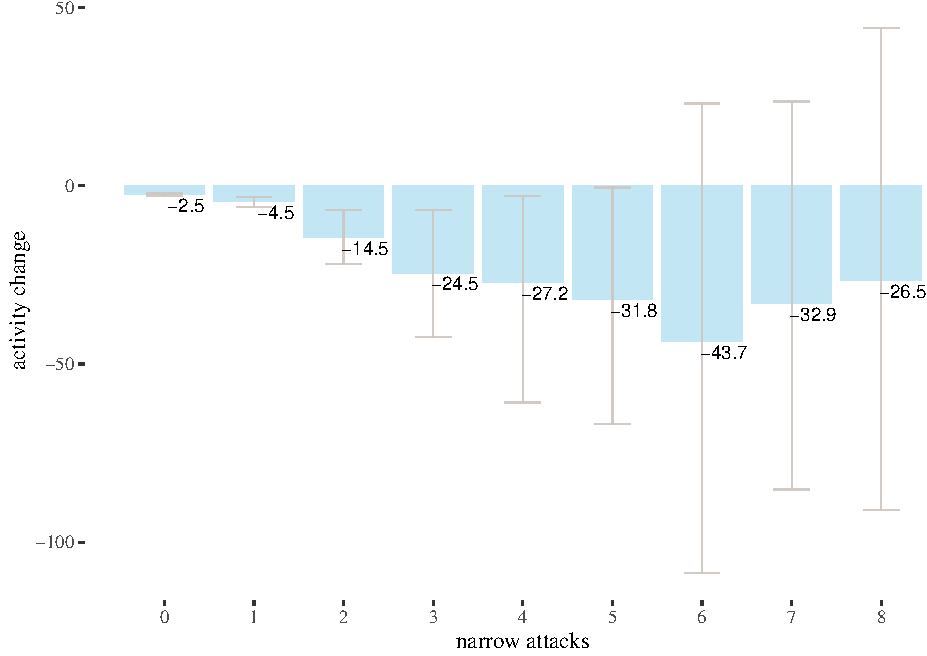
\includegraphics[width=1\linewidth]{redditAnalysisWalkthrough_files/figure-latex/unnamed-chunk-58-1} \end{center}
\end{subfigure} 


\begin{subfigure}[!ht]{0.9\textwidth}

\begin{center}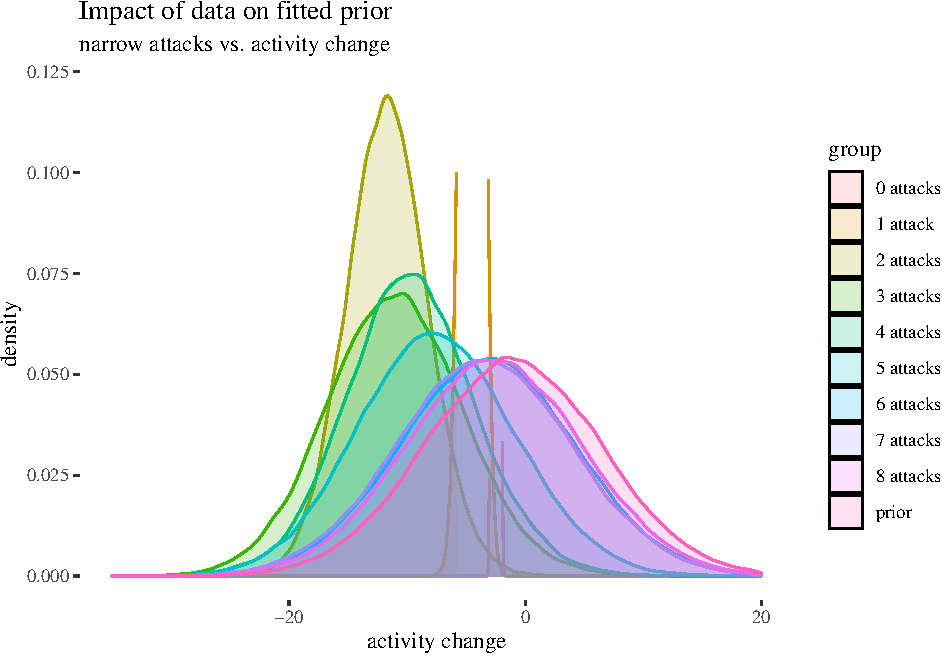
\includegraphics[width=1\linewidth]{redditAnalysisWalkthrough_files/figure-latex/unnamed-chunk-59-1} \end{center}
\end{subfigure}


\caption{Prior and posterior distributions for all attacks and wide priors, with posterior means and HDI limits in barplots.}
\label{fig:bayesian1}
\end{figure}

\begin{figure}[!ht]
\begin{subfigure}[!ht]{0.9\textwidth}

\begin{center}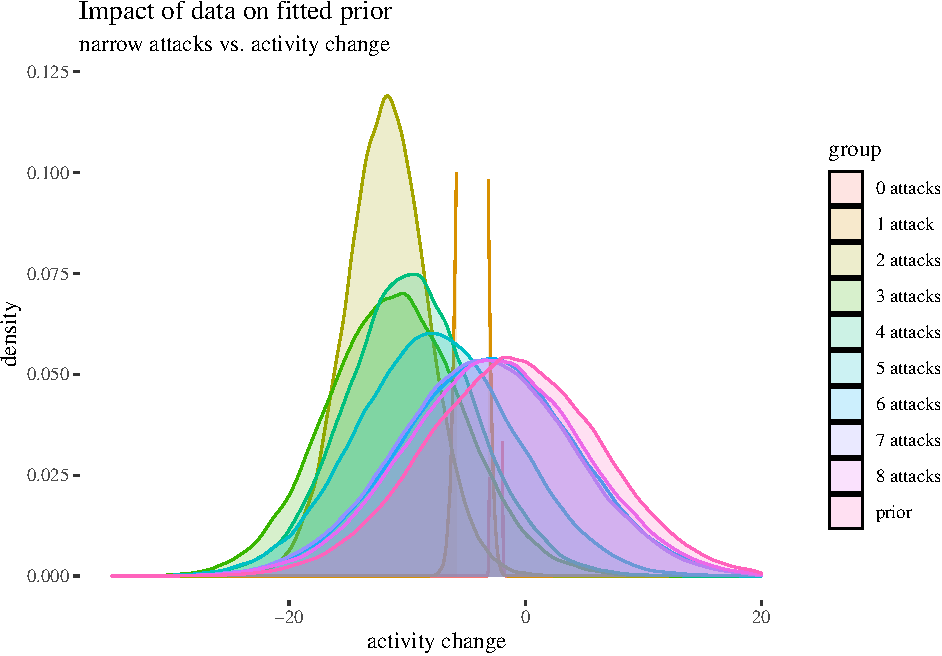
\includegraphics[width=1\linewidth]{redditAnalysisWalkthrough_files/figure-latex/unnamed-chunk-60-1} \end{center}
\end{subfigure} 


\begin{subfigure}[!ht]{0.9\textwidth}

\begin{center}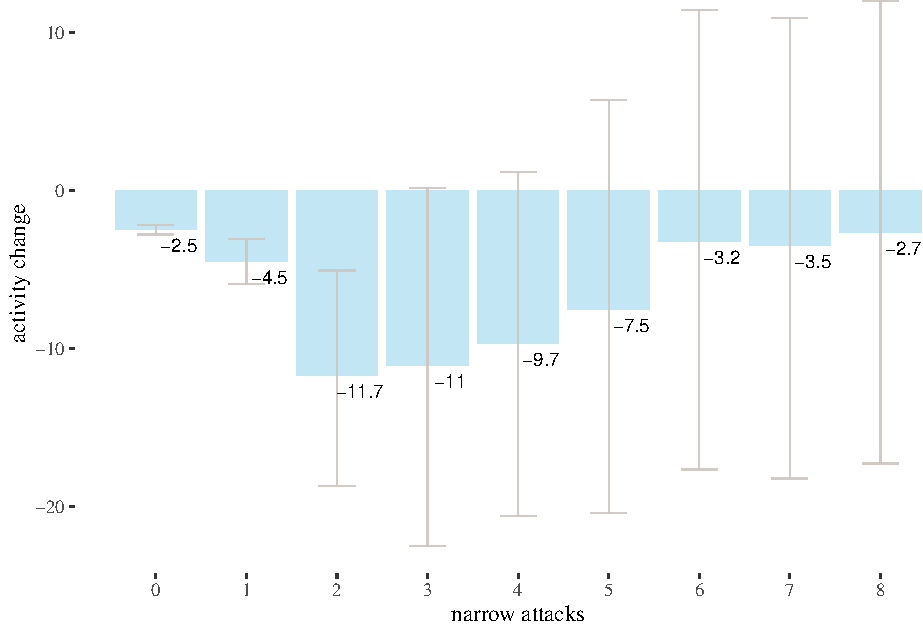
\includegraphics[width=1\linewidth]{redditAnalysisWalkthrough_files/figure-latex/unnamed-chunk-61-1} \end{center}
\end{subfigure}
\caption{Prior and posterior distributions for all attacks and fitted priors, with posterior means and HDI limits in barplots.}
\label{fig:bayesian2}
\end{figure}

\begin{figure}[!ht]
\begin{subfigure}[!ht]{0.9\textwidth}

\begin{center}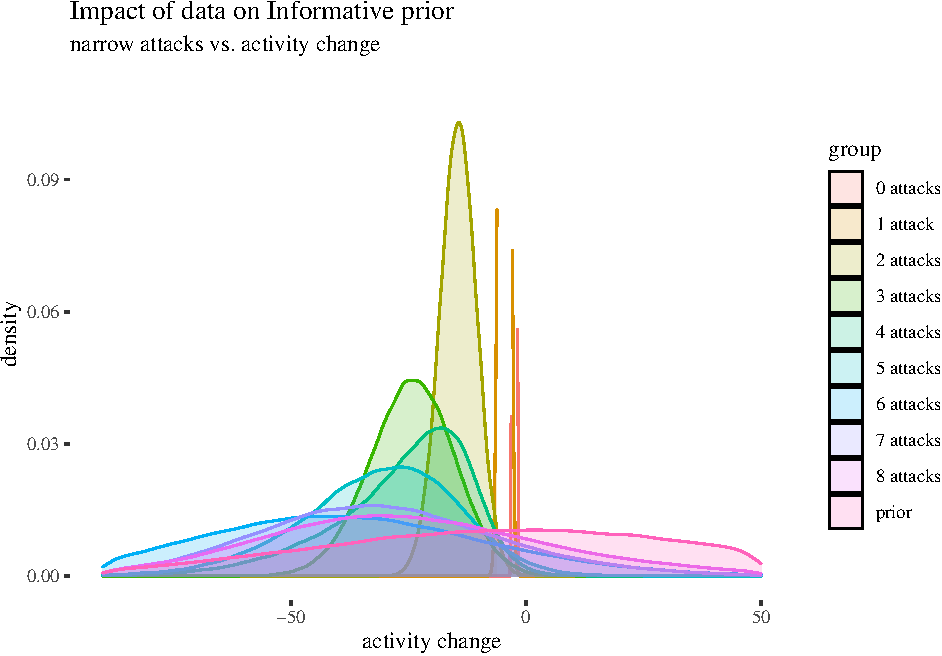
\includegraphics[width=1\linewidth]{redditAnalysisWalkthrough_files/figure-latex/unnamed-chunk-62-1} \end{center}
\end{subfigure} 


\begin{subfigure}[!ht]{0.9\textwidth}

\begin{center}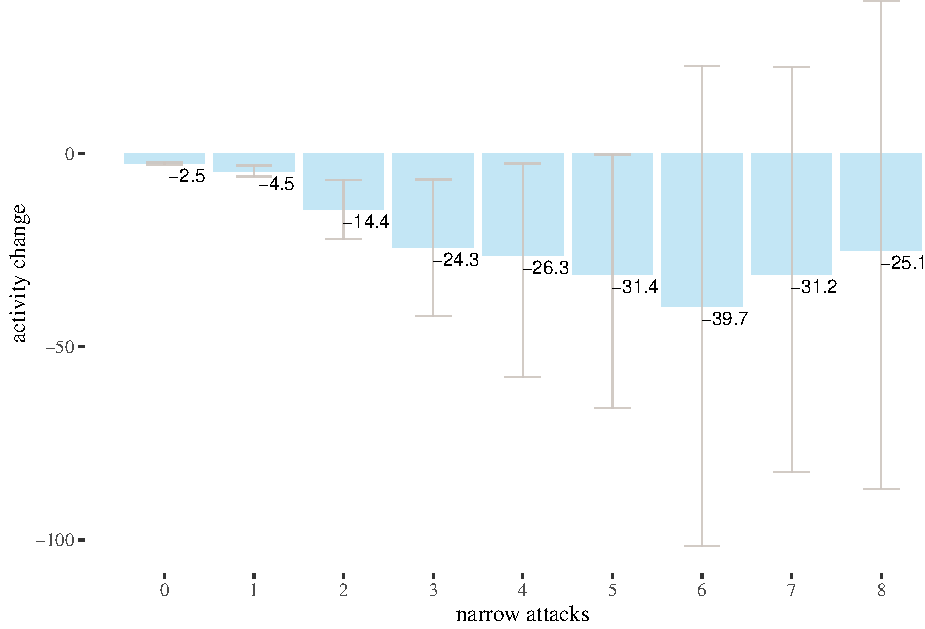
\includegraphics[width=1\linewidth]{redditAnalysisWalkthrough_files/figure-latex/unnamed-chunk-63-1} \end{center}
\end{subfigure}

\caption{Prior and posterior distributions for all attacks and informative priors, with posterior means and HDI limits in barplots.}
\label{fig:bayesian3}
\end{figure}

\normalsize

The near-vertical lines represent the density for 0 attacks, which goes
high up --- plotting the whole range of \(y\) axis would make the rest
of the plot unintelligible. As the number of attacks grow, no matter
which prior we start with, the posterior means move left (which agrees
with the results we obtained with other methods) and the density plots
become wider. This is partially because the groups become smaller as the
number of attacks increases, and partially because the standard
deviations between the groups are uneven (users who received more
attacks seem to display more uneven behavior).

\begin{figure}[!ht]

\begin{center}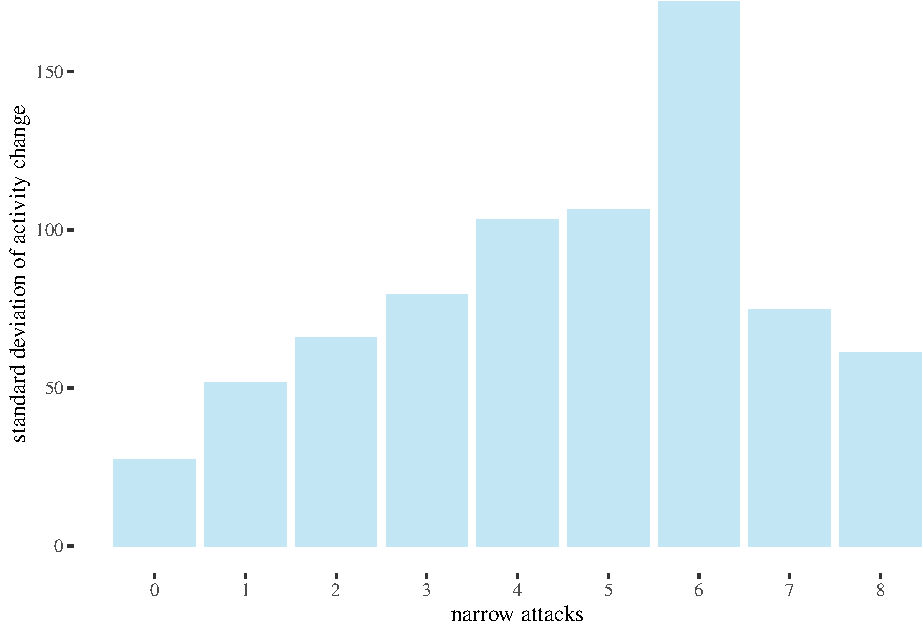
\includegraphics[width=1\linewidth]{redditAnalysisWalkthrough_files/figure-latex/unnamed-chunk-64-1} \end{center}
\caption{Standard deviations of  activity change vs. narrow attacks.}
\label{fig:bayesian3'}
\end{figure}

\section{Model-theoretic analysis}

\normalsize

We analyzed the correlation between attacks received and activity change
using classical and bayesian methods. However, there is a number of
predictors we have not yet used. The impact of some of them, such as the
number of attacks on \emph{posts} written by an author, could provide
further insight. More importantly, some of them might be confounding
variables. Crucially, since previous activity seems to be a good
predictor of future activity and since high number of attacks received
in the \textsf{before} period correlates with high activity before, one
might be concerned that whatever explaining the value of high attacks
before does in our analysis should actually be attributed simply to
activity.

To reach some clarity on such issues, we perform a regression analysis
to see how the predictors in best fit models interact, and to use the
model parameters to get some comparison of the impact they have. We
build a number of potentially viable generalized linear regression
models meant to predict \textsf{activityAfter} based on a selection of
other variables, pick the best one(s) and analyze what they reveal about
the predictors involved.

\footnotesize

\begin{Shaded}
\begin{Highlighting}[]
\KeywordTok{library}\NormalTok{(MASS)}
\KeywordTok{library}\NormalTok{(vcd)}
\KeywordTok{library}\NormalTok{(lmtest)}
\KeywordTok{library}\NormalTok{(countreg)}
\KeywordTok{library}\NormalTok{(pscl)}
\KeywordTok{library}\NormalTok{(stats)}
\end{Highlighting}
\end{Shaded}

\normalsize

Our first challenge was finding the right distribution for the outcome
variable (Figure \ref{fig:activityDistro}).

\footnotesize

\begin{Shaded}
\begin{Highlighting}[]
\NormalTok{activityAfterTab <-}\StringTok{ }\KeywordTok{table}\NormalTok{(}\KeywordTok{factor}\NormalTok{(data}\OperatorTok{$}\NormalTok{activityAfter, }\DataTypeTok{levels =} \DecValTok{0}\OperatorTok{:}\KeywordTok{max}\NormalTok{(data}\OperatorTok{$}\NormalTok{activityAfter)))}
\NormalTok{activityAfterDf <-}\StringTok{ }\KeywordTok{as.data.frame}\NormalTok{(activityAfterTab)}
\NormalTok{activityAfterDf}\OperatorTok{$}\NormalTok{Var1 <-}\StringTok{ }\KeywordTok{as.integer}\NormalTok{(activityAfterDf}\OperatorTok{$}\NormalTok{Var1)}
\end{Highlighting}
\end{Shaded}

\begin{Shaded}
\begin{Highlighting}[]
\NormalTok{activityDistr <-}\StringTok{ }\KeywordTok{ggplot}\NormalTok{(activityAfterDf, }\KeywordTok{aes}\NormalTok{(}\DataTypeTok{x =}\NormalTok{ Var1, }\DataTypeTok{y =}\NormalTok{ Freq)) }\OperatorTok{+}
\StringTok{    }\KeywordTok{geom_bar}\NormalTok{(}\DataTypeTok{stat =} \StringTok{"identity"}\NormalTok{) }\OperatorTok{+}\StringTok{ }\KeywordTok{scale_x_continuous}\NormalTok{(}\DataTypeTok{breaks =} \KeywordTok{seq}\NormalTok{(}\DecValTok{0}\NormalTok{,}
    \DecValTok{1000}\NormalTok{, }\DataTypeTok{by =} \DecValTok{50}\NormalTok{)) }\OperatorTok{+}\StringTok{ }\NormalTok{th }\OperatorTok{+}\StringTok{ }\KeywordTok{labs}\NormalTok{(}\DataTypeTok{title =} \StringTok{"Distribution of activityAfter"}\NormalTok{) }\OperatorTok{+}
\StringTok{    }\KeywordTok{xlab}\NormalTok{(}\StringTok{"activityAfter"}\NormalTok{) }\OperatorTok{+}\StringTok{ }\KeywordTok{ylab}\NormalTok{(}\StringTok{"count"}\NormalTok{)}

\NormalTok{activityDistrRestr <-}\StringTok{ }\KeywordTok{ggplot}\NormalTok{(activityAfterDf, }\KeywordTok{aes}\NormalTok{(}\DataTypeTok{x =}\NormalTok{ Var1, }\DataTypeTok{y =}\NormalTok{ Freq)) }\OperatorTok{+}
\StringTok{    }\KeywordTok{geom_bar}\NormalTok{(}\DataTypeTok{stat =} \StringTok{"identity"}\NormalTok{) }\OperatorTok{+}\StringTok{ }\KeywordTok{scale_x_continuous}\NormalTok{(}\DataTypeTok{breaks =} \KeywordTok{seq}\NormalTok{(}\DecValTok{0}\NormalTok{,}
    \DecValTok{100}\NormalTok{, }\DataTypeTok{by =} \DecValTok{10}\NormalTok{), }\DataTypeTok{limits =} \KeywordTok{c}\NormalTok{(}\DecValTok{0}\NormalTok{, }\DecValTok{100}\NormalTok{)) }\OperatorTok{+}\StringTok{ }\NormalTok{th }\OperatorTok{+}\StringTok{ }\KeywordTok{labs}\NormalTok{(}\DataTypeTok{title =} \StringTok{"Distribution of activityAfter"}\NormalTok{,}
    \DataTypeTok{subtitle =} \StringTok{"x restricted to 0-100"}\NormalTok{) }\OperatorTok{+}\StringTok{ }\KeywordTok{xlab}\NormalTok{(}\StringTok{"activityAfter"}\NormalTok{) }\OperatorTok{+}
\StringTok{    }\KeywordTok{ylab}\NormalTok{(}\StringTok{"count"}\NormalTok{)}
\end{Highlighting}
\end{Shaded}

\normalsize

\begin{figure}
\begin{subfigure}[b]{0.45\textwidth}

\begin{center}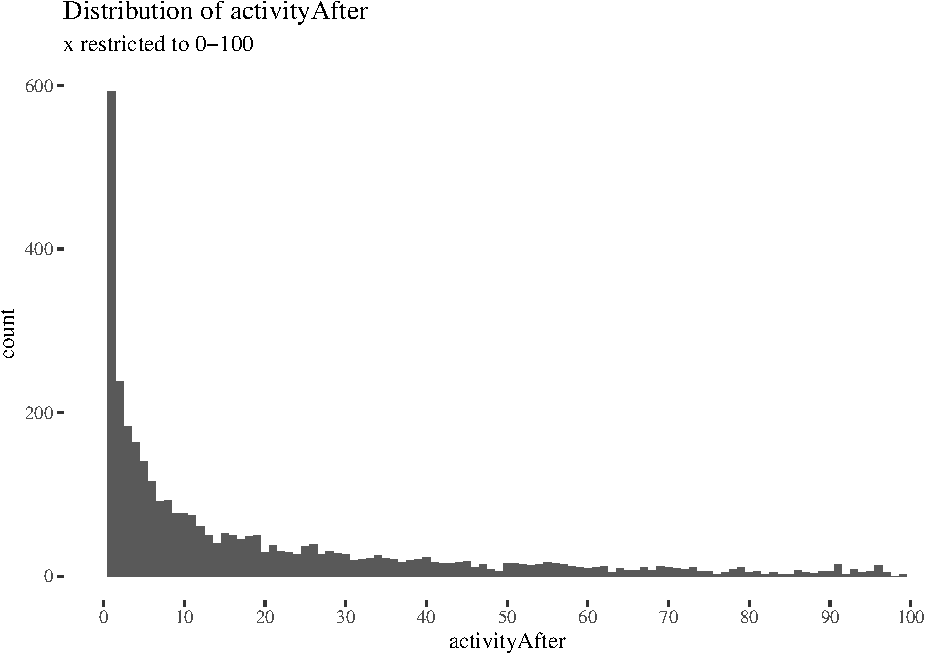
\includegraphics[width=1\linewidth]{redditAnalysisWalkthrough_files/figure-latex/unnamed-chunk-68-1} \end{center}
\end{subfigure}
\begin{subfigure}[b]{0.45\textwidth}

\begin{center}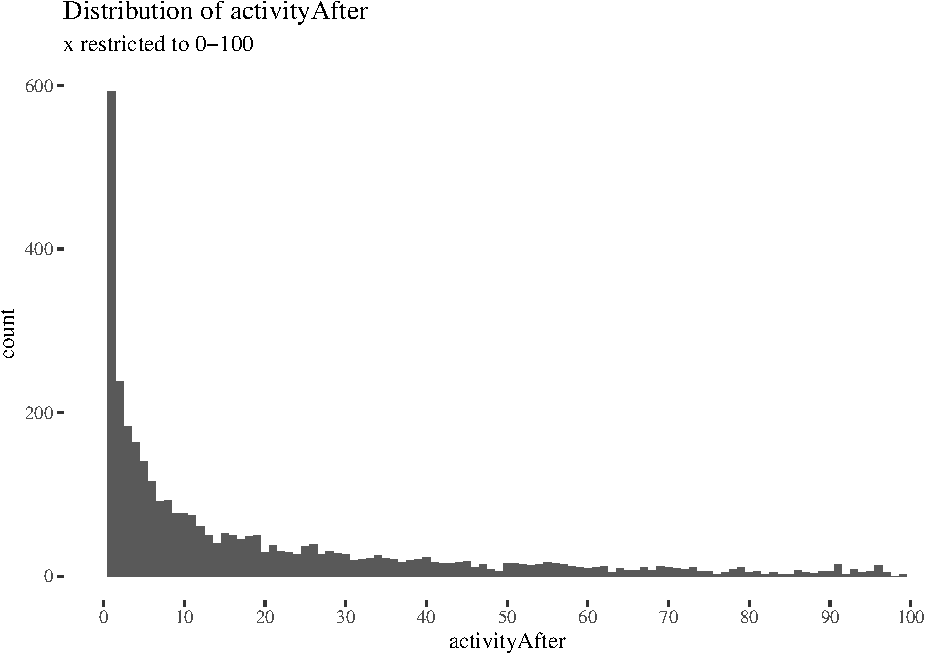
\includegraphics[width=1\linewidth]{redditAnalysisWalkthrough_files/figure-latex/unnamed-chunk-69-1} \end{center}
\end{subfigure}
\caption{Empirical distribution of activityAfter}
\label{fig:activityDistro}
\end{figure}

\footnotesize

\begin{Shaded}
\begin{Highlighting}[]
\NormalTok{activityFitPois <-}\StringTok{ }\KeywordTok{goodfit}\NormalTok{(activityAfterTab, }\DataTypeTok{type =} \StringTok{"poisson"}\NormalTok{)}
\KeywordTok{unlist}\NormalTok{(activityFitPois}\OperatorTok{$}\NormalTok{par)}
\KeywordTok{summary}\NormalTok{(activityFitPois)}
\end{Highlighting}
\end{Shaded}

\normalsize 

One potential candidate was the Poisson distribution. We identified the
Poisson distribution that best fits the data, used its \(\lambda\)
parameter (\(\approx 35.69\)) to perform a goodness-of-fit test (with
\(df=273\), \(\chi^2 \approx \infty\) and \(P(>\chi^2)\approx 0\)), and
compare visually the predicted values with the actual ones.

\footnotesize

\begin{Shaded}
\begin{Highlighting}[]
\NormalTok{activityFitPois <-}\StringTok{ }\KeywordTok{goodfit}\NormalTok{(activityAfterTab, }\DataTypeTok{type =} \StringTok{"poisson"}\NormalTok{)}
\NormalTok{poissonFitPlot <-}\StringTok{ }\KeywordTok{ggplot}\NormalTok{(activityAfterDf, }\KeywordTok{aes}\NormalTok{(}\DataTypeTok{x =}\NormalTok{ Var1, }\DataTypeTok{y =}\NormalTok{ Freq)) }\OperatorTok{+}
\StringTok{    }\KeywordTok{geom_bar}\NormalTok{(}\DataTypeTok{stat =} \StringTok{"identity"}\NormalTok{, }\DataTypeTok{alpha =} \FloatTok{0.6}\NormalTok{) }\OperatorTok{+}\StringTok{ }\KeywordTok{scale_x_continuous}\NormalTok{(}\DataTypeTok{breaks =} \KeywordTok{seq}\NormalTok{(}\DecValTok{0}\NormalTok{,}
    \DecValTok{100}\NormalTok{, }\DataTypeTok{by =} \DecValTok{10}\NormalTok{), }\DataTypeTok{limits =} \KeywordTok{c}\NormalTok{(}\DecValTok{0}\NormalTok{, }\DecValTok{100}\NormalTok{)) }\OperatorTok{+}\StringTok{ }\NormalTok{th }\OperatorTok{+}\StringTok{ }\KeywordTok{labs}\NormalTok{(}\DataTypeTok{title =} \StringTok{"activityAfter with fitted best Poisson model predictions"}\NormalTok{,}
    \DataTypeTok{subtitle =} \StringTok{"x restricted to 0-100"}\NormalTok{) }\OperatorTok{+}\StringTok{ }\KeywordTok{xlab}\NormalTok{(}\StringTok{"activityAfter"}\NormalTok{) }\OperatorTok{+}
\StringTok{    }\KeywordTok{ylab}\NormalTok{(}\StringTok{"count"}\NormalTok{) }\OperatorTok{+}\StringTok{ }\KeywordTok{geom_point}\NormalTok{(}\KeywordTok{aes}\NormalTok{(}\DataTypeTok{x =}\NormalTok{ Var1, }\DataTypeTok{y =}\NormalTok{ activityFitPois}\OperatorTok{$}\NormalTok{fitted),}
    \DataTypeTok{colour =} \StringTok{"darksalmon"}\NormalTok{, }\DataTypeTok{size =} \FloatTok{0.5}\NormalTok{, }\DataTypeTok{alpha =} \FloatTok{0.5}\NormalTok{)}
\end{Highlighting}
\end{Shaded}

\normalsize

\begin{figure}

\begin{center}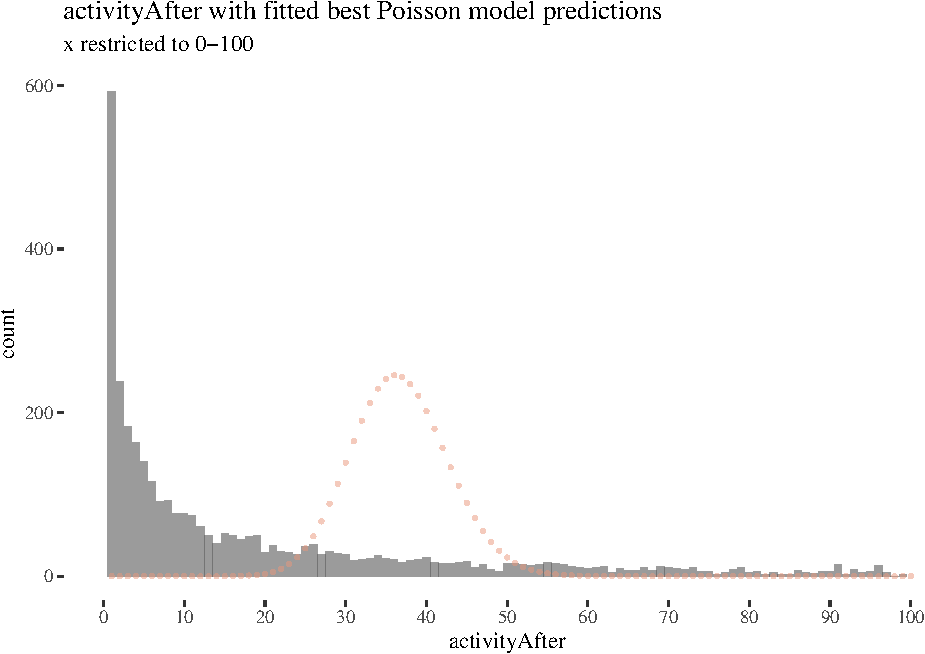
\includegraphics[width=1\linewidth]{redditAnalysisWalkthrough_files/figure-latex/unnamed-chunk-72-1} \end{center}
\caption{Poor performance of best-fitting Poisson distribution.}
\end{figure}

There were at least two problems: zero-inflation and overspread. The
former means that the model predicts much fewer zeros than there really
are in the data, and the latter means that the model predicts fewer
higher values than there are in the data. The best fitting \(\lambda\)
was fairly high and moved the highest values of Poisson too far to the
right compared to where they were expected. Over-dispersion could be
handled by moving to a quasi-Poisson distribution, but this would not
help us much with the zero counts.

\footnotesize

\begin{Shaded}
\begin{Highlighting}[]
\NormalTok{activityFitNbin <-}\StringTok{ }\KeywordTok{goodfit}\NormalTok{(activityAfterTab, }\DataTypeTok{type =} \StringTok{"nbinom"}\NormalTok{)}
\KeywordTok{summary}\NormalTok{(activityFitNbin)}
\end{Highlighting}
\end{Shaded}

\begin{Shaded}
\begin{Highlighting}[]
\NormalTok{activityFitNbin <-}\StringTok{ }\KeywordTok{goodfit}\NormalTok{(activityAfterTab, }\DataTypeTok{type =} \StringTok{"nbinom"}\NormalTok{)}
\NormalTok{poissonNbinPlot2 <-}\StringTok{ }\KeywordTok{ggplot}\NormalTok{(activityAfterDf, }\KeywordTok{aes}\NormalTok{(}\DataTypeTok{x =}\NormalTok{ Var1, }\DataTypeTok{y =}\NormalTok{ Freq)) }\OperatorTok{+}
\StringTok{    }\KeywordTok{geom_bar}\NormalTok{(}\DataTypeTok{stat =} \StringTok{"identity"}\NormalTok{, }\DataTypeTok{alpha =} \FloatTok{0.5}\NormalTok{) }\OperatorTok{+}\StringTok{ }\KeywordTok{scale_x_continuous}\NormalTok{(}\DataTypeTok{breaks =} \KeywordTok{seq}\NormalTok{(}\DecValTok{0}\NormalTok{,}
    \DecValTok{100}\NormalTok{, }\DataTypeTok{by =} \DecValTok{10}\NormalTok{), }\DataTypeTok{limits =} \KeywordTok{c}\NormalTok{(}\DecValTok{0}\NormalTok{, }\DecValTok{100}\NormalTok{)) }\OperatorTok{+}\StringTok{ }\NormalTok{th }\OperatorTok{+}\StringTok{ }\KeywordTok{labs}\NormalTok{(}\DataTypeTok{title =} \StringTok{"activityAfter with fitted best negative binomial model predictions"}\NormalTok{,}
    \DataTypeTok{subtitle =} \StringTok{"x restricted to 0-100"}\NormalTok{) }\OperatorTok{+}\StringTok{ }\KeywordTok{xlab}\NormalTok{(}\StringTok{"activityAfter"}\NormalTok{) }\OperatorTok{+}
\StringTok{    }\KeywordTok{ylab}\NormalTok{(}\StringTok{"count"}\NormalTok{) }\OperatorTok{+}\StringTok{ }\KeywordTok{geom_point}\NormalTok{(}\KeywordTok{aes}\NormalTok{(}\DataTypeTok{x =}\NormalTok{ Var1, }\DataTypeTok{y =}\NormalTok{ activityFitNbin}\OperatorTok{$}\NormalTok{fitted),}
    \DataTypeTok{colour =} \StringTok{"darksalmon"}\NormalTok{, }\DataTypeTok{size =} \FloatTok{0.5}\NormalTok{, }\DataTypeTok{alpha =} \FloatTok{0.8}\NormalTok{)}
\end{Highlighting}
\end{Shaded}

\normalsize 

\begin{figure}

\begin{center}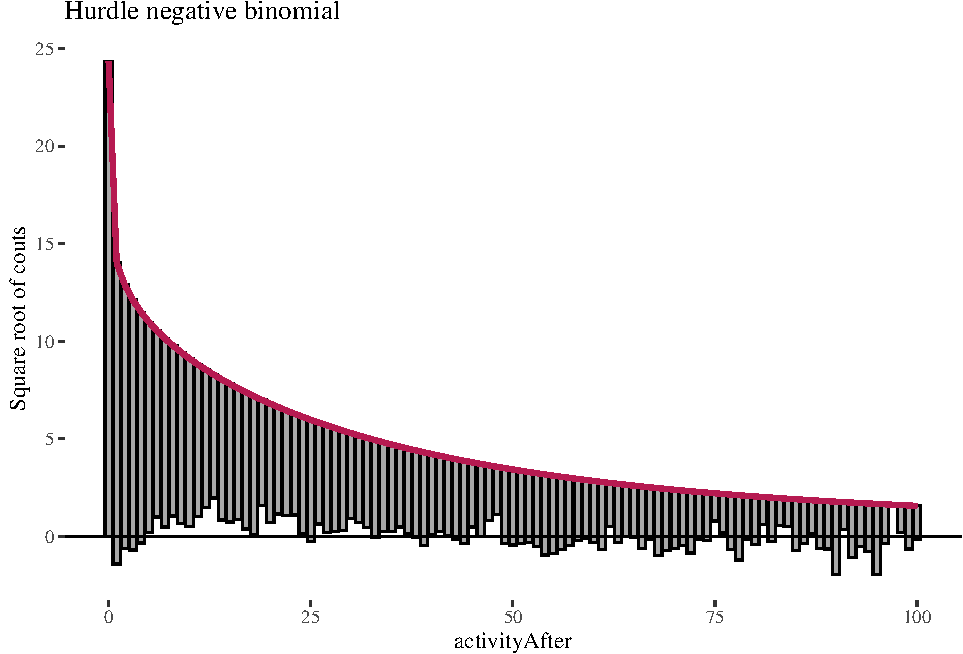
\includegraphics[width=1\linewidth]{redditAnalysisWalkthrough_files/figure-latex/unnamed-chunk-75-1} \end{center}
\caption{Somewhat better performance of best-fitting negative binomial distribution.}
\label{fig:nbinperf}
\end{figure}

Another candidate distribution we considered was negative binomial.
There still were problems with zeros although in the opposite direction
though), the goodness-of-fit test resulted in \(\chi^2 \approx 647\) and
\(P(>\chi^s)\approx 0\), but the right side of the Figure
\ref{fig:nbinperf} looks better. This suggested that improvements were
still needed.

There are two well-known strategies to develop distributions for data
with high zero counts: zero-inflated and hurdle models. In a
zero-inflated Poisson (ZIP) model (Lambert 1992) a distinction is made
between the structural zeros for which the output value will always be
0, and the rest, sometimes giving random zeros. A ZIP model is comprised
of two components:

\begin{itemize}
\item  A model for the binary event of membership in the class where 0 is necessary. Typically, this is logistic regression. 

\item  A Poisson (or negative binomial) model for the remaining observed count, potentially including some zeros as well. Typically a log link is used to predict the mean.
\end{itemize}

In hurdle models (proposed initially by Cragg (1971) and developed
further by Mullahy (1986)) the idea is that there may be some special
``hurdle'' required to reach a positive count. The model uses:

\begin{itemize}
\item A logistic regression  submodel to distinguish counts of zero from larger counts, and
\item  Truncated Poisson (or negative binomial) regression for the positive counts  excluding the zero counts.
\end{itemize}

We start with the full predictor sets. We display rootograms (they have
\emph{squared} frequencies on the \(y\)-axis to increase the visibility
of lower counts) for the models (Figure \ref{fig:rootograms}).

\footnotesize

\begin{Shaded}
\begin{Highlighting}[]
\NormalTok{data}\OperatorTok{$}\NormalTok{sumLowOnlyBefore <-}\StringTok{ }\NormalTok{data}\OperatorTok{$}\NormalTok{sumLowBefore }\OperatorTok{-}\StringTok{ }\NormalTok{data}\OperatorTok{$}\NormalTok{sumHighBefore}

\NormalTok{fullModelZINbin <-}\StringTok{ }\KeywordTok{zeroinfl}\NormalTok{(activityAfter }\OperatorTok{~}\StringTok{ }\NormalTok{sumLowOnlyBefore }\OperatorTok{+}
\StringTok{    }\NormalTok{sumHighBefore }\OperatorTok{+}\StringTok{ }\NormalTok{sumPlBefore }\OperatorTok{+}\StringTok{ }\NormalTok{sumPhBefore }\OperatorTok{+}\StringTok{ }\NormalTok{activityBefore,}
    \DataTypeTok{data =}\NormalTok{ data, }\DataTypeTok{dist =} \StringTok{"negbin"}\NormalTok{)}

\NormalTok{fullModelHNbin <-}\StringTok{ }\KeywordTok{hurdle}\NormalTok{(activityAfter }\OperatorTok{~}\StringTok{ }\NormalTok{sumLowOnlyBefore }\OperatorTok{+}\StringTok{ }\NormalTok{sumHighBefore }\OperatorTok{+}
\StringTok{    }\NormalTok{sumPlBefore }\OperatorTok{+}\StringTok{ }\NormalTok{sumPhBefore }\OperatorTok{+}\StringTok{ }\NormalTok{activityBefore, }\DataTypeTok{data =}\NormalTok{ data,}
    \DataTypeTok{dist =} \StringTok{"negbin"}\NormalTok{)}

\NormalTok{fullModelZIpois <-}\StringTok{ }\KeywordTok{zeroinfl}\NormalTok{(activityAfter }\OperatorTok{~}\StringTok{ }\NormalTok{sumLowOnlyBefore }\OperatorTok{+}
\StringTok{    }\NormalTok{sumHighBefore }\OperatorTok{+}\StringTok{ }\NormalTok{sumPlBefore }\OperatorTok{+}\StringTok{ }\NormalTok{sumPhBefore }\OperatorTok{+}\StringTok{ }\NormalTok{activityBefore,}
    \DataTypeTok{data =}\NormalTok{ data, }\DataTypeTok{dist =} \StringTok{"poisson"}\NormalTok{)}

\NormalTok{fullModelHpois <-}\StringTok{ }\KeywordTok{hurdle}\NormalTok{(activityAfter }\OperatorTok{~}\StringTok{ }\NormalTok{sumLowOnlyBefore }\OperatorTok{+}\StringTok{ }\NormalTok{sumHighBefore }\OperatorTok{+}
\StringTok{    }\NormalTok{sumPlBefore }\OperatorTok{+}\StringTok{ }\NormalTok{sumPhBefore }\OperatorTok{+}\StringTok{ }\NormalTok{activityBefore, }\DataTypeTok{data =}\NormalTok{ data,}
    \DataTypeTok{dist =} \StringTok{"poisson"}\NormalTok{)}
\end{Highlighting}
\end{Shaded}

\normalsize

\begin{figure}[h!]
\begin{subfigure}[b]{0.45\textwidth}

\begin{center}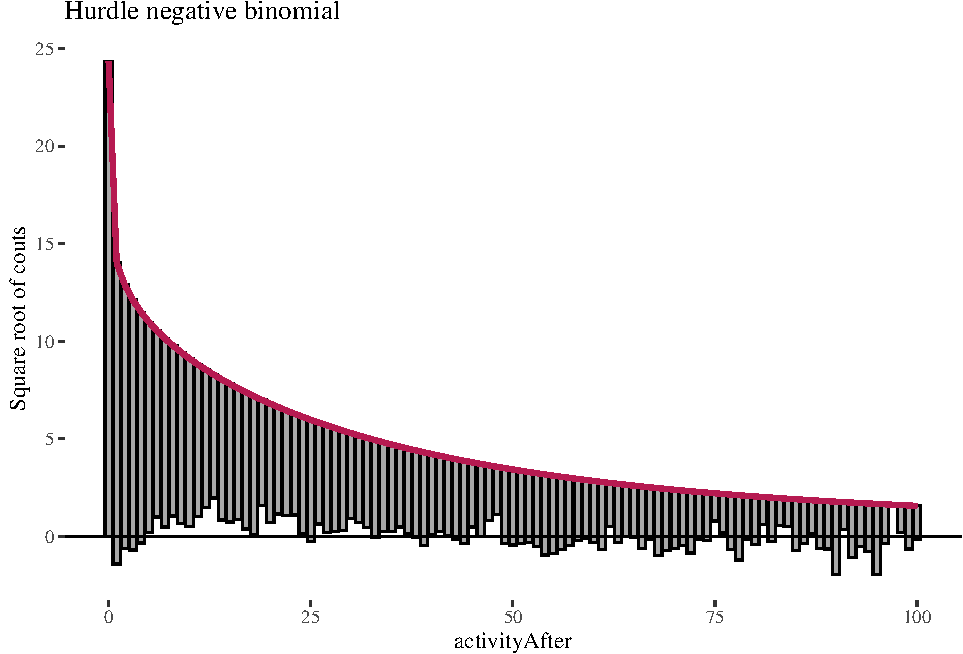
\includegraphics[width=1\linewidth]{redditAnalysisWalkthrough_files/figure-latex/unnamed-chunk-78-1} \end{center}
\end{subfigure}
\hfill
\begin{subfigure}[b]{0.45\textwidth}

\begin{center}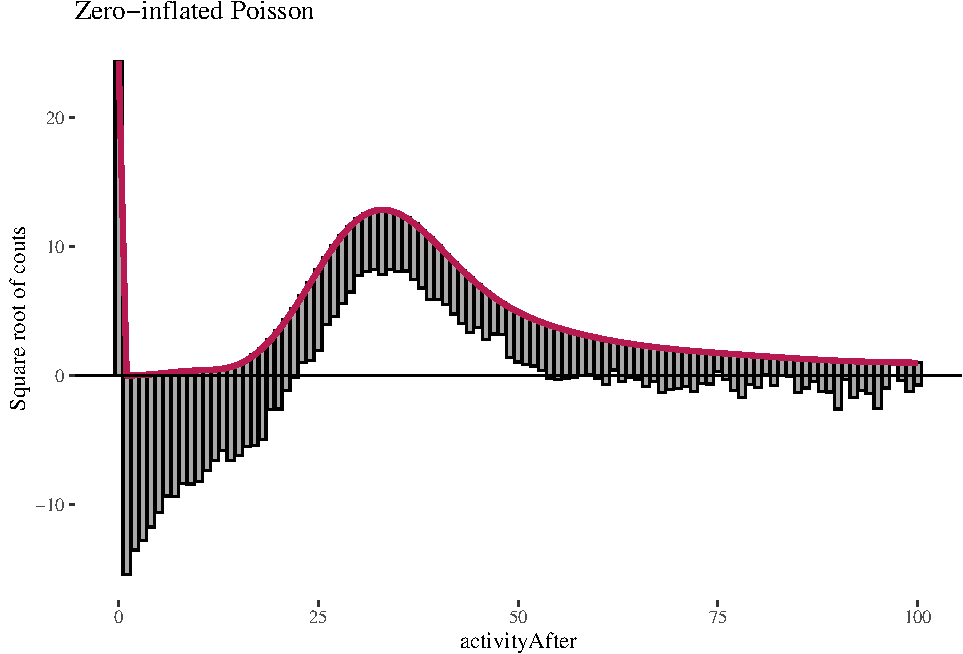
\includegraphics[width=1\linewidth]{redditAnalysisWalkthrough_files/figure-latex/unnamed-chunk-79-1} \end{center}
\end{subfigure}

\begin{subfigure}[b]{0.45\textwidth}

\begin{center}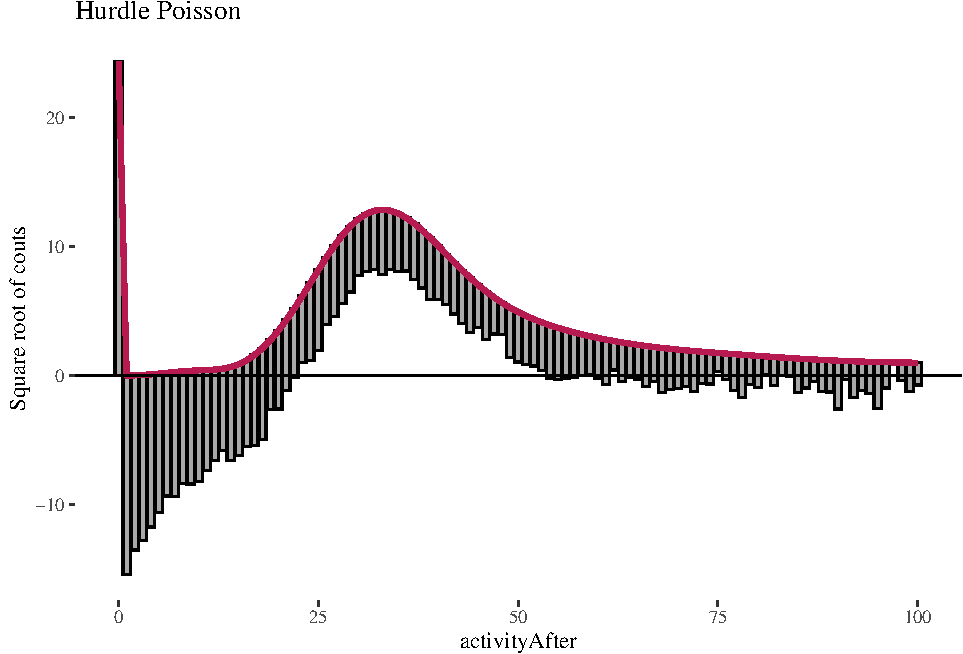
\includegraphics[width=1\linewidth]{redditAnalysisWalkthrough_files/figure-latex/unnamed-chunk-80-1} \end{center}
\end{subfigure}
\hfill
\begin{subfigure}[b]{0.45\textwidth}

\begin{center}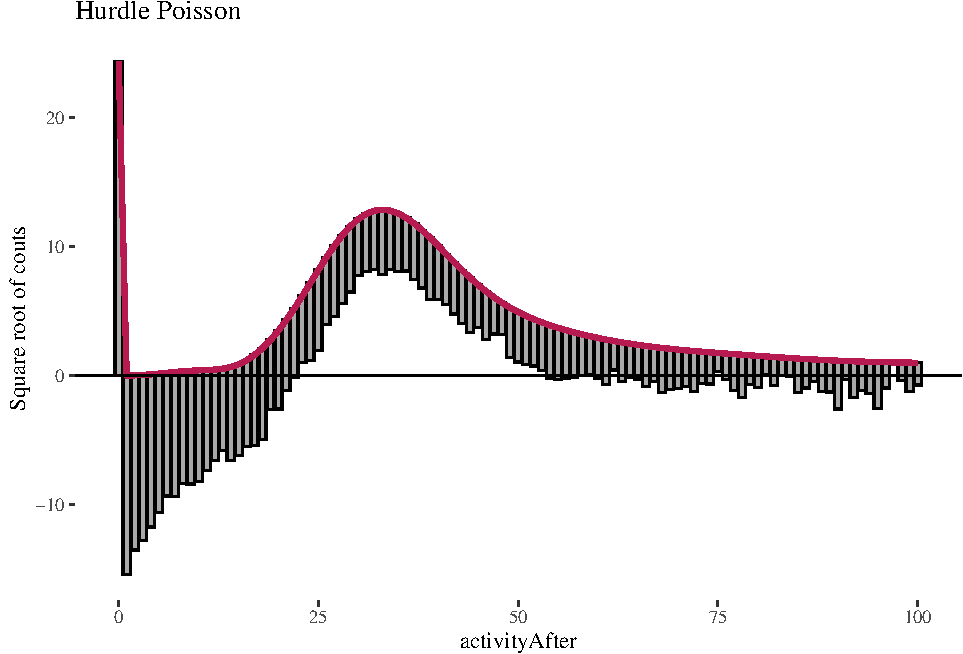
\includegraphics[width=1\linewidth]{redditAnalysisWalkthrough_files/figure-latex/unnamed-chunk-81-1} \end{center}
\end{subfigure}
\caption{Rootograms for four candidate zero-handling distributions; note the y axes are squared counts.}
\label{fig:rootograms}
\end{figure}

The first observation was that even zero-inflation or hurdling do not
improve the Poisson distribution much. The second was that once we use
negative binomial distribution, it does not seem to make much of a
difference whether we use zero-inflation or hurdling. We investigated
this further. One method of comparing such models is the Vuong test
which produced \(z\)-statistic (\(2.08\) with \(p\approx 0.018\))
suggesting the zero-inflated negative binomial model is better than
hurdle negative binomial. However, the differences in log-likelihood
(14459 vs.~14527) and AIC (28945 vs.~29081) were not large.

\footnotesize

\begin{Shaded}
\begin{Highlighting}[]
\KeywordTok{vuong}\NormalTok{(fullModelZINbin, fullModelHNbin)}
\end{Highlighting}
\end{Shaded}

\begin{Shaded}
\begin{Highlighting}[]
\KeywordTok{logLik}\NormalTok{(fullModelZINbin)}
\KeywordTok{AIC}\NormalTok{(fullModelZINbin)}

\KeywordTok{logLik}\NormalTok{(fullModelHNbin)}
\KeywordTok{AIC}\NormalTok{(fullModelHNbin)}
\end{Highlighting}
\end{Shaded}

\normalsize

There seem to be some reasons to prefer the zero-inflated model, but the
score differences are not too impressive, both likelihood ratios are
Akaike scores are very close (note: we want to minimize AIC and maximize
log likelihood).

To move on we need to modify the variables, because some of the counts
included others. This was not a problem so far, but now we will be
looking in detail at their roles jointly, and so it is important to not
count various things multiple times.

\footnotesize

\begin{Shaded}
\begin{Highlighting}[]
\CommentTok{# select variables of interest}
\NormalTok{dataModeling <-}\StringTok{ }\NormalTok{data }\OperatorTok
\StringTok{    }\NormalTok{dplyr}\OperatorTok{::}\KeywordTok{select}\NormalTok{(sumLowOnlyBefore, sumHighBefore, sumPlBefore,}
\NormalTok{        sumPhBefore, activityBefore, activityAfter)}

\CommentTok{# sum narrow now becomes sum of narrow attacks on comments}
\NormalTok{dataModeling}\OperatorTok{$}\NormalTok{sumHighBefore <-}\StringTok{ }\NormalTok{dataModeling}\OperatorTok{$}\NormalTok{sumHighBefore }\OperatorTok{-}\StringTok{ }\NormalTok{dataModeling}\OperatorTok{$}\NormalTok{sumPhBefore}

\CommentTok{# sum wide only now becomes sum of wide only on comments}
\NormalTok{dataModeling}\OperatorTok{$}\NormalTok{sumLowOnlyBefore <-}\StringTok{ }\NormalTok{dataModeling}\OperatorTok{$}\NormalTok{sumLowOnlyBefore }\OperatorTok{-}
\StringTok{    }\NormalTok{dataModeling}\OperatorTok{$}\NormalTok{sumPlBefore}

\CommentTok{# sum of wide on posts now becomes sum of wide only on}
\CommentTok{# posts}
\NormalTok{dataModeling}\OperatorTok{$}\NormalTok{sumPlBefore <-}\StringTok{ }\NormalTok{dataModeling}\OperatorTok{$}\NormalTok{sumPlBefore }\OperatorTok{-}\StringTok{ }\NormalTok{dataModeling}\OperatorTok{$}\NormalTok{sumPhBefore}
\end{Highlighting}
\end{Shaded}

\normalsize

We build zero-inflated negative binomial and hurdle negative binomial
models, one with all variables, and one based on previous activity only.
If we can get equally good predictions using previous activity only and
ignoring information about attacks, this would suggest no impact of the
other variables.

\footnotesize 

\begin{Shaded}
\begin{Highlighting}[]
\NormalTok{ZNBfull <-}\StringTok{ }\KeywordTok{zeroinfl}\NormalTok{(activityAfter }\OperatorTok{~}\StringTok{ }\NormalTok{., }\DataTypeTok{data =}\NormalTok{ dataModeling, }\DataTypeTok{dist =} \StringTok{"negbin"}\NormalTok{)}
\NormalTok{ZNBactivity <-}\StringTok{ }\KeywordTok{zeroinfl}\NormalTok{(activityAfter }\OperatorTok{~}\StringTok{ }\NormalTok{activityBefore, }\DataTypeTok{data =}\NormalTok{ dataModeling,}
    \DataTypeTok{dist =} \StringTok{"negbin"}\NormalTok{)}
\NormalTok{HNBfull <-}\StringTok{ }\KeywordTok{hurdle}\NormalTok{(activityAfter }\OperatorTok{~}\StringTok{ }\NormalTok{., }\DataTypeTok{data =}\NormalTok{ dataModeling, }\DataTypeTok{dist =} \StringTok{"negbin"}\NormalTok{)}
\NormalTok{HNBactivity <-}\StringTok{ }\KeywordTok{hurdle}\NormalTok{(activityAfter }\OperatorTok{~}\StringTok{ }\NormalTok{activityBefore, }\DataTypeTok{data =}\NormalTok{ dataModeling,}
    \DataTypeTok{dist =} \StringTok{"negbin"}\NormalTok{)}

\CommentTok{# now take a look at this}
\KeywordTok{summary}\NormalTok{(dataModeling}\OperatorTok{$}\NormalTok{activityAfter)}
\end{Highlighting}
\end{Shaded}

\begin{verbatim}
##    Min. 1st Qu.  Median    Mean 3rd Qu.    Max. 
##    0.00    2.00   10.00   35.69   38.00 1032.00
\end{verbatim}

\normalsize

The outcome variable has third quartile of weekly activity count in the
\textsf{after} period at 38, and we are mostly interested in predictive
accuracy where most of the users are placed. Therefore, we look at what
happens with these models up to 40 (Figure \ref{fig:rootogramsFeature}).

\footnotesize

\normalsize

\begin{figure}
\begin{subfigure}[b]{0.45\textwidth}

\begin{center}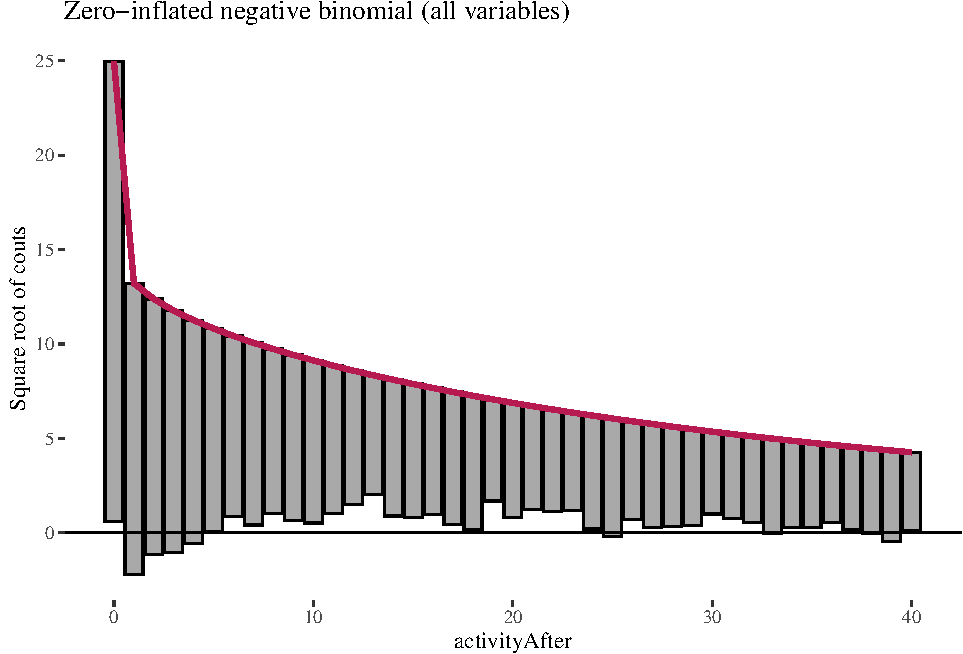
\includegraphics[width=1\linewidth]{redditAnalysisWalkthrough_files/figure-latex/unnamed-chunk-87-1} \end{center}
\end{subfigure}
\hfill
\begin{subfigure}[b]{0.45\textwidth}

\begin{center}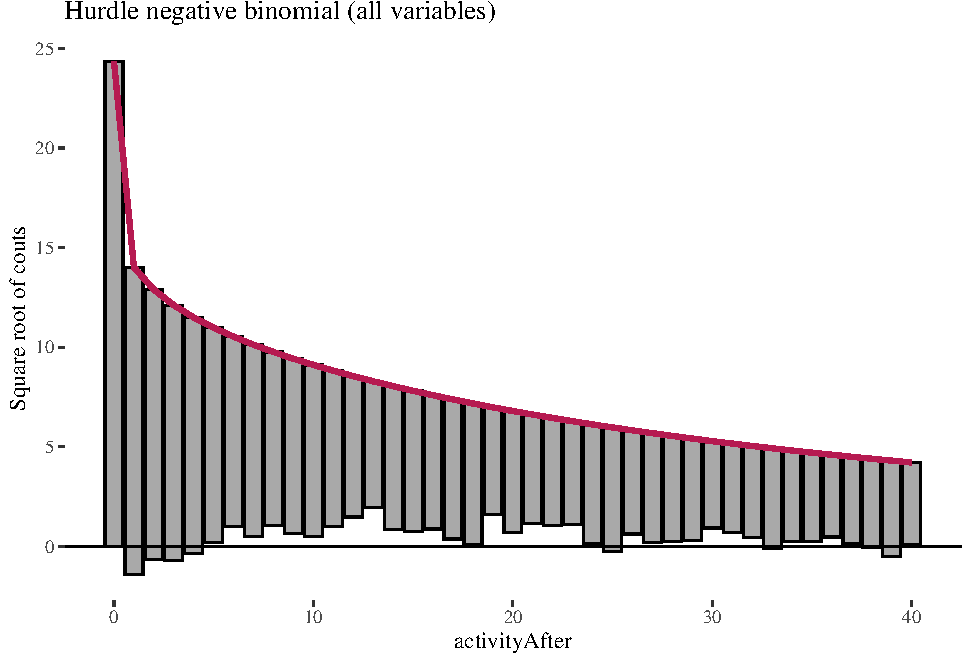
\includegraphics[width=1\linewidth]{redditAnalysisWalkthrough_files/figure-latex/unnamed-chunk-88-1} \end{center}
\end{subfigure}

\begin{subfigure}[b]{0.45\textwidth}

\begin{center}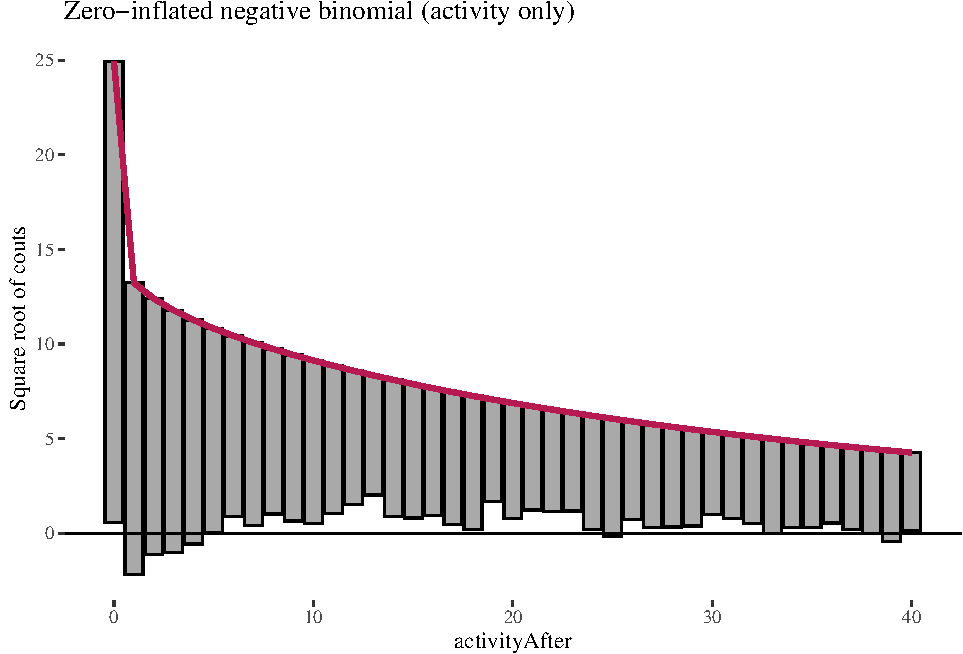
\includegraphics[width=1\linewidth]{redditAnalysisWalkthrough_files/figure-latex/unnamed-chunk-89-1} \end{center}
\end{subfigure}
\hfill
\begin{subfigure}[b]{0.45\textwidth}

\begin{center}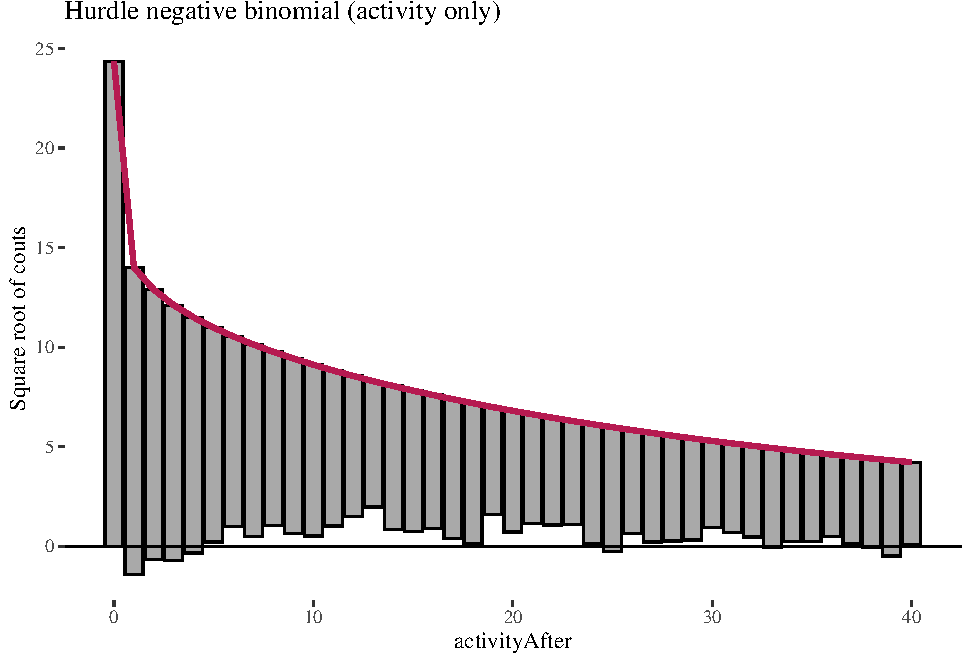
\includegraphics[width=1\linewidth]{redditAnalysisWalkthrough_files/figure-latex/unnamed-chunk-90-1} \end{center}
\end{subfigure}
\caption{Rootograms for all variables vs. activity only with zero-inflated and hurdle models.}
\label{fig:rootogramsFeature}
\end{figure}

Here, zero-inflated models under-predict low non-zero counts, while
hurdle models are a bit better in this respect, so we will focus on
them. It is more difficult to see any important difference between the
two hurdle models. We compare them using likelihood ratio test. For each
selection of variables, we first pick the value of parameters in the
model that maximizes the probability density of the data given this
choice of variables and these parameters (likelihood). We do this for
two nested models, then we take the log of the ratio of these, and we
get a measure of how well, comparatively, they fit the data. Moreover,
multiplying this ratio by -2, we obtain a statistic that has a
\(\chi^2\) distribution, which can be further used to r calculate the
p-value for the null hypothesis that the added variables make no
difference.

Log-likelihood test results in \(\chi^2 \approx 20.28\), with
\(P(>\chi^2)\approx 0.009\). Wald's test is somewhat similar (ableit
more generally applicable). It also indicates that the additional
variables are significant (\(\chi^2 \approx 24.71\) with
\(P(>\chi^2)\approx 0.0017\)), which suggests that variables other than
previous activity are also significant. Finally, Akaike Information
Criterion (Akaike, 1974) provides an estimator of out-of-sample
prediction error and penalizes more complex models. As long as we
evaluate models with respect to the same data, the ones with lower
Akaike score should be chosen. Even with penalty for the additional
variables, the full model receives better score (although the difference
is not very large, 29,081 vs.~29,085).

First, we can do this in a step-wise manner:

\footnotesize

\begin{Shaded}
\begin{Highlighting}[]
\KeywordTok{library}\NormalTok{(lmtest)}
\NormalTok{likHNBactivity <-}\StringTok{ }\KeywordTok{logLik}\NormalTok{(HNBactivity)}
\NormalTok{likHNBfull <-}\StringTok{ }\KeywordTok{logLik}\NormalTok{(HNBfull)}
\NormalTok{(teststat <-}\StringTok{ }\DecValTok{-2} \OperatorTok{*}\StringTok{ }\NormalTok{(}\KeywordTok{as.numeric}\NormalTok{(likHNBactivity) }\OperatorTok{-}\StringTok{ }\KeywordTok{as.numeric}\NormalTok{(likHNBfull)))}
\end{Highlighting}
\end{Shaded}

\begin{verbatim}
## [1] 20.28267
\end{verbatim}

\begin{Shaded}
\begin{Highlighting}[]
\NormalTok{df <-}\StringTok{ }\DecValTok{13} \OperatorTok{-}\StringTok{ }\DecValTok{5}
\NormalTok{(p.val <-}\StringTok{ }\KeywordTok{pchisq}\NormalTok{(teststat, }\DataTypeTok{df =}\NormalTok{ df, }\DataTypeTok{lower.tail =} \OtherTok{FALSE}\NormalTok{))}
\end{Highlighting}
\end{Shaded}

\begin{verbatim}
## [1] 0.009317915
\end{verbatim}

\normalsize

The same result can be achieved more quickly using the following lines:

\footnotesize

\begin{Shaded}
\begin{Highlighting}[]
\KeywordTok{waldtest}\NormalTok{(HNBactivity, HNBfull)}
\end{Highlighting}
\end{Shaded}

\begin{Shaded}
\begin{Highlighting}[]
\KeywordTok{AIC}\NormalTok{(HNBactivity)}
\KeywordTok{AIC}\NormalTok{(HNBfull)}
\end{Highlighting}
\end{Shaded}

\normalsize

Next, we inspect the HNB model (Tables \ref{tab:fhnb_estimates1} and
\ref{tab:fhnb_estimates2}) and interpret the result.

\footnotesize

\begin{Shaded}
\begin{Highlighting}[]
\KeywordTok{library}\NormalTok{(stargazer)}
\KeywordTok{stargazer}\NormalTok{(HNBfull)}
\end{Highlighting}
\end{Shaded}

\normalsize 

\begin{table}[!h] \centering
\begin{tabular}{@{\extracolsep{5pt}}lc}
\\[-1.8ex]\hline
\hline \\[-1.8ex]
& \multicolumn{1}{c}{\textit{Dependent variable:}} \\
\cline{2-2}
\\[-1.8ex] & activityAfter \\
\hline \\[-1.8ex]
sumLowOnlyBefore & $-$0.009 \\
& (0.014) \\
& \\
sumHighBefore & $-$0.008 \\
& (0.020) \\
& \\
sumPlBefore & 0.015 \\
& (0.013) \\
& \\
sumPhBefore & $-$0.139$^{**}$ \\
& (0.069) \\
& \\
activityBefore & 0.015$^{***}$ \\
& (0.001) \\
& \\
Constant & 2.534$^{***}$ \\
& (0.032) \\
& \\
\hline \\[-1.8ex]
Observations & 3,673 \\
Log Likelihood & $-$14,527.690 \\
\hline
\hline \\[-1.8ex]
\textit{Note:} & \multicolumn{1}{r}{$^{*}$p$<$0.1; $^{**}$p$<$0.05; $^{***}$p$<$0.01} \\
\end{tabular}
\caption{Estimated parameters of the full hurdle negative binomial model.}
\label{tab:fhnb_estimates}
\end{table}

\begin{table}[!h] \centering
\begin{tabular}{@{\extracolsep{5pt}}lc}
\\[-1.8ex]\hline
\hline \\[-1.8ex]
& \multicolumn{1}{c}{\textit{Dependent variable:}} \\
\cline{2-2}
\\[-1.8ex] & activityAfter \\
\hline \\[-1.8ex]
sumLowOnlyBefore & $-$0.009 \\
& (0.53) \\
& \\
sumHighBefore & $-$0.008 \\
& (0.7) \\
& \\
sumPlBefore & 0.024 \\
& (0.21) \\
& \\
sumPhBefore & $-$0.147 \\
& (0.07) \\
& \\
activityBefore & 0.015$^{***}$ \\
& (2e-16) \\
& \\
Constant & 2.534$^{***}$ \\
& (2e-16) \\
& \\
\hline
\hline \\[-1.8ex]
\textit{Note:} & \multicolumn{1}{r}{$^{*}$p$<$0.1; $^{**}$p$<$0.05; $^{***}$p$<$0.01} \\
\end{tabular}
\caption{Estimated parameters of the count part of the  hurdle negative binomial model.}
\label{tab:fhnb_estimates1}
\end{table}

\begin{table}[!h] \centering
\begin{tabular}{@{\extracolsep{5pt}}lc}
\\[-1.8ex]\hline
\hline \\[-1.8ex]
& \multicolumn{1}{c}{\textit{Dependent variable:}} \\
\cline{2-2}
\\[-1.8ex] & activityAfter \\
\hline \\[-1.8ex]
sumLowOnlyBefore & $-$0.009 \\
& (0.81) \\
& \\
sumHighBefore & $-$0.111 \\
& (0.32) \\
& \\
sumPlBefore & -0.094 \\
& (0.04)$^{*}$ \\
& \\
sumPhBefore & $0.36^{*}$ \\
& (0.03) \\
& \\
activityBefore & 0.08$^{***}$ \\
& (2e-16) \\
& \\
Constant & 0.49$^{***}$ \\
& (5.04e-13) \\
& \\
\hline
\hline \\[-1.8ex]
\textit{Note:} & \multicolumn{1}{r}{$^{*}$p$<$0.1; $^{**}$p$<$0.05; $^{***}$p$<$0.01} \\
\end{tabular}
\caption{Estimated parameters of the zero  part of the  hurdle negative binomial model.}
\label{tab:fhnb_estimates2}
\end{table}

\normalsize

The output is split into two submodels: one for predicting zeros, one
for the counts. It could be suggested to ignore those variables whose
coefficients are not statistically significant, but given the already
discussed reasons to include these variables, we are not going to do
this (in fact, attaching too much value to statistical significance
thresholds can be pernicious, and also misleading if the predictors are
correlated, as attacks on posts and attacks on comments may well be).
Moreover, the results of step-wise elimination from the full model are
sensitive to the ordering in which we consider variables, and there is
no principled reason to prefer any of the orderings. Instead,
interpreting \(p\)-values we apply the following advice: the closer it
is to 1, the more skeptical we should be about the judgment the model
makes about its
role.\footnote{See the excellent book titled \emph{The Cult of Statistical Significance: How the Standard Error Costs Us Jobs, Justice, and Lives} by Stephen T. Ziliak and Deirdre N. McCloskey.}
The coefficeints are somewhat difficult to interpret because the models
use log link function. Therefore we first exponentiate them to obtain
odds ratios:

\footnotesize

\begin{Shaded}
\begin{Highlighting}[]
\NormalTok{expCoef <-}\StringTok{ }\KeywordTok{as.data.frame}\NormalTok{(}\KeywordTok{round}\NormalTok{((}\KeywordTok{exp}\NormalTok{(}\KeywordTok{coef}\NormalTok{((HNBfull)))), }\DecValTok{3}\NormalTok{))}
\KeywordTok{colnames}\NormalTok{(expCoef) <-}\StringTok{ }\KeywordTok{c}\NormalTok{(}\StringTok{"Odds ratios"}\NormalTok{)}
\KeywordTok{mykable}\NormalTok{(expCoef)}
\end{Highlighting}
\end{Shaded}

\begin{table}
\centering\begingroup\fontsize{9}{11}\selectfont

\begin{tabular}{lr}
\toprule
  & Odds ratios\\
\midrule
\cellcolor{gray!6}{count\_(Intercept)} & \cellcolor{gray!6}{12.606}\\
count\_sumLowOnlyBefore & 0.991\\
\cellcolor{gray!6}{count\_sumHighBefore} & \cellcolor{gray!6}{0.992}\\
count\_sumPlBefore & 1.015\\
\cellcolor{gray!6}{count\_sumPhBefore} & \cellcolor{gray!6}{0.870}\\
\addlinespace
count\_activityBefore & 1.015\\
\cellcolor{gray!6}{zero\_(Intercept)} & \cellcolor{gray!6}{1.634}\\
zero\_sumLowOnlyBefore & 0.990\\
\cellcolor{gray!6}{zero\_sumHighBefore} & \cellcolor{gray!6}{0.894}\\
zero\_sumPlBefore & 0.901\\
\addlinespace
\cellcolor{gray!6}{zero\_sumPhBefore} & \cellcolor{gray!6}{1.156}\\
zero\_activityBefore & 1.084\\
\bottomrule
\end{tabular}
\endgroup{}
\end{table}

\normalsize

Next we analyze the intercepts of the count submodel. The baseline
number of posts for those who are not in the zero class is 12.6. The
coefficients indicate that the multiplicative contribution of each unit
change. For instance:

\begin{itemize}
\item Each additional wide only attack on a user decreases the baseline by factor of .991. So, other things being equal, receiving 10 wide attacks only would decrease  a user's activity by $100 \times (1-.991^{10}) \approx 8.6\%$.
\item The impact of narrow attacks on comments is similar.
\item Interestingly, wide only attacks on post actually increase activity, at least for those who are not in the zero class. For instance, four of them would increase the activity by $100\times (1-1.006^4) \approx 2.4\%$.
\item The strongest impact is due to narrow only attacks on posts. Even one of them decreases one's expected activity by $14\%$, thus, receiving  receiving five of them  reduces one's expected activity by $50\%$. 
\end{itemize}

Next, regarding the zero submodel.

\begin{itemize}
\item The basic odds for not posting for the whole week are 1.63. This means that the probability of belonging to the zero class is $\nicefrac{1.63\,}{1+1.63}\approx 0.61$.
\item wide only attacks, narrow attacks on comments, wide only attacks on posts all decrease the chances in being in the zero class.
\item In contrast, receiving narrow attacks on posts has a  strong impact, increasing the chances of not posting anything next week. For instance, with the baseline odds 1.63, if one receives five such attacks, other things being equal, her chances of not posting for a week go to $\frac{(1.63\times 1.15^5 }{1+(1.63\times 1.15^5)}\approx .76$.
\item Interestingly, posting in the previous week makes one slightly more likely to not post the next week. One's baseline probability of being active, $1-0.61 = 0.39$ goes to   $1-\frac{1.63 \times 1.08^20}{1+1.63 \times 1.08^20} \approx 0.22$ if in the preceding week one wrote on \textsf{Reddit} 20 times, other things being equal. 
\end{itemize}

We visualise the effects of selected variables by plotting what activity
levels the model predicts for their different values (we focus on 0-40,
as the top of this range is already an extrapolation), while keeping
other variables fixed at their mean values (Figure \ref{fig:effects}).

\footnotesize

\begin{Shaded}
\begin{Highlighting}[]
\NormalTok{sumLowOnlyBefore <-}\StringTok{ }\KeywordTok{rep}\NormalTok{(}\KeywordTok{mean}\NormalTok{(dataModeling}\OperatorTok{$}\NormalTok{sumLowOnlyBefore),}
    \DecValTok{4001}\NormalTok{)}
\NormalTok{sumHighBefore <-}\StringTok{ }\KeywordTok{rep}\NormalTok{(}\KeywordTok{mean}\NormalTok{(dataModeling}\OperatorTok{$}\NormalTok{sumHighBefore), }\DecValTok{4001}\NormalTok{)}
\NormalTok{sumPlBefore <-}\StringTok{ }\KeywordTok{rep}\NormalTok{(}\KeywordTok{mean}\NormalTok{(dataModeling}\OperatorTok{$}\NormalTok{sumPlBefore), }\DecValTok{4001}\NormalTok{)}
\NormalTok{sumPhBefore <-}\StringTok{ }\KeywordTok{rep}\NormalTok{(}\KeywordTok{mean}\NormalTok{(dataModeling}\OperatorTok{$}\NormalTok{sumPhBefore), }\DecValTok{4001}\NormalTok{)}
\NormalTok{activityBefore <-}\StringTok{ }\KeywordTok{rep}\NormalTok{(}\KeywordTok{mean}\NormalTok{(dataModeling}\OperatorTok{$}\NormalTok{activityBefore), }\DecValTok{4001}\NormalTok{)}
\NormalTok{activityAfter <-}\StringTok{ }\KeywordTok{rep}\NormalTok{(}\KeywordTok{mean}\NormalTok{(dataModeling}\OperatorTok{$}\NormalTok{activityAfter), }\DecValTok{4001}\NormalTok{)}

\NormalTok{baseEffDf <-}\StringTok{ }\KeywordTok{data.frame}\NormalTok{(sumLowOnlyBefore, sumHighBefore, sumPlBefore,}
\NormalTok{    sumPhBefore, activityBefore, activityAfter)}

\NormalTok{effSizePlot <-}\StringTok{ }\ControlFlowTok{function}\NormalTok{(columnno, }\DataTypeTok{range =} \DecValTok{40}\NormalTok{, }\DataTypeTok{by =} \DecValTok{5}\NormalTok{) \{}
\NormalTok{    EffDf <-}\StringTok{ }\NormalTok{baseEffDf}
\NormalTok{    EffDf[, columnno] <-}\StringTok{ }\DecValTok{0}\OperatorTok{:}\DecValTok{4000}
\NormalTok{    EffDf}\OperatorTok{$}\NormalTok{prediction <-}\StringTok{ }\KeywordTok{predict}\NormalTok{(HNBfull, EffDf)}
    \KeywordTok{ggplot}\NormalTok{(EffDf, }\KeywordTok{aes}\NormalTok{(}\DataTypeTok{x =}\NormalTok{ EffDf[, columnno], }\DataTypeTok{y =}\NormalTok{ prediction)) }\OperatorTok{+}
\StringTok{        }\KeywordTok{geom_smooth}\NormalTok{(}\DataTypeTok{alpha =} \FloatTok{0.5}\NormalTok{, }\DataTypeTok{col =} \StringTok{"skyblue"}\NormalTok{, }\DataTypeTok{se =} \OtherTok{FALSE}\NormalTok{) }\OperatorTok{+}
\StringTok{        }\KeywordTok{scale_x_continuous}\NormalTok{(}\DataTypeTok{breaks =} \KeywordTok{seq}\NormalTok{(}\DecValTok{0}\NormalTok{, range, }\DataTypeTok{by =}\NormalTok{ by), }\DataTypeTok{limits =} \KeywordTok{c}\NormalTok{(}\OperatorTok{-}\DecValTok{1}\NormalTok{,}
\NormalTok{            range)) }\OperatorTok{+}\StringTok{ }\NormalTok{th }\OperatorTok{+}\StringTok{ }\KeywordTok{ylab}\NormalTok{(}\StringTok{"predicted activity"}\NormalTok{)}
\NormalTok{\}}

\NormalTok{effLO <-}\StringTok{ }\KeywordTok{effSizePlot}\NormalTok{(}\DecValTok{1}\NormalTok{, }\DecValTok{500}\NormalTok{, }\DecValTok{50}\NormalTok{)  }\CommentTok{#low only}
\NormalTok{effH <-}\StringTok{ }\KeywordTok{effSizePlot}\NormalTok{(}\DecValTok{2}\NormalTok{, }\DecValTok{50}\NormalTok{, }\DecValTok{5}\NormalTok{)  }\CommentTok{#narrow on comments}
\NormalTok{effPl <-}\StringTok{ }\KeywordTok{effSizePlot}\NormalTok{(}\DecValTok{3}\NormalTok{, }\DecValTok{100}\NormalTok{, }\DecValTok{10}\NormalTok{)  }\CommentTok{#pl}
\NormalTok{effPh <-}\StringTok{ }\KeywordTok{effSizePlot}\NormalTok{(}\DecValTok{4}\NormalTok{, }\DecValTok{50}\NormalTok{, }\DecValTok{5}\NormalTok{)  }\CommentTok{#ph}
\NormalTok{effA <-}\StringTok{ }\KeywordTok{effSizePlot}\NormalTok{(}\DecValTok{5}\NormalTok{, }\DecValTok{200}\NormalTok{, }\DecValTok{20}\NormalTok{)  }\CommentTok{#abefore}
\end{Highlighting}
\end{Shaded}

\normalsize

\begin{figure}
\begin{subfigure}[b]{0.45\textwidth}

\begin{center}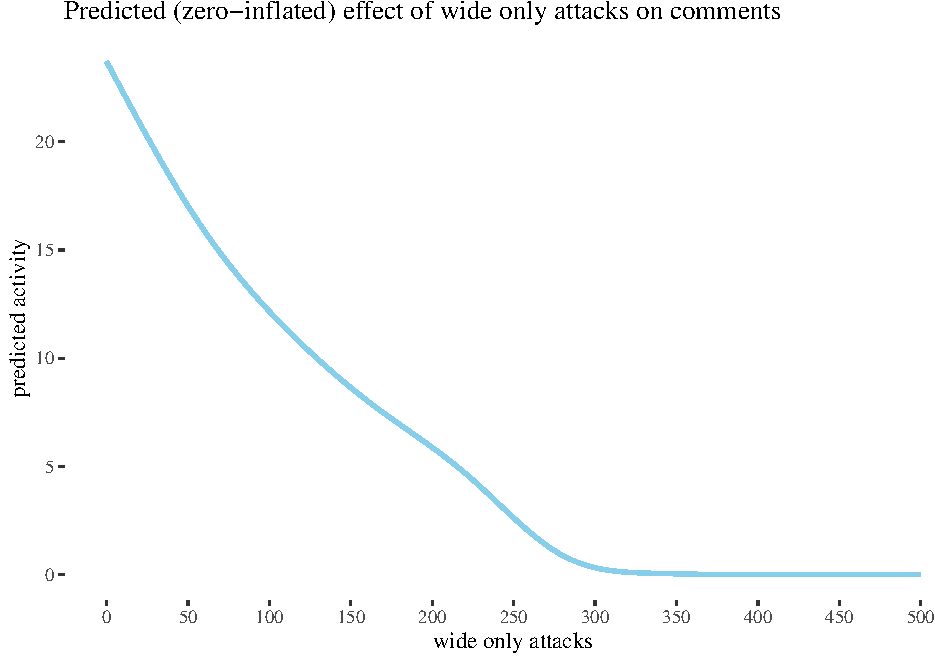
\includegraphics[width=1\linewidth]{redditAnalysisWalkthrough_files/figure-latex/unnamed-chunk-98-1} \end{center}
\end{subfigure}
\hfill
\begin{subfigure}[b]{0.45\textwidth}

\begin{center}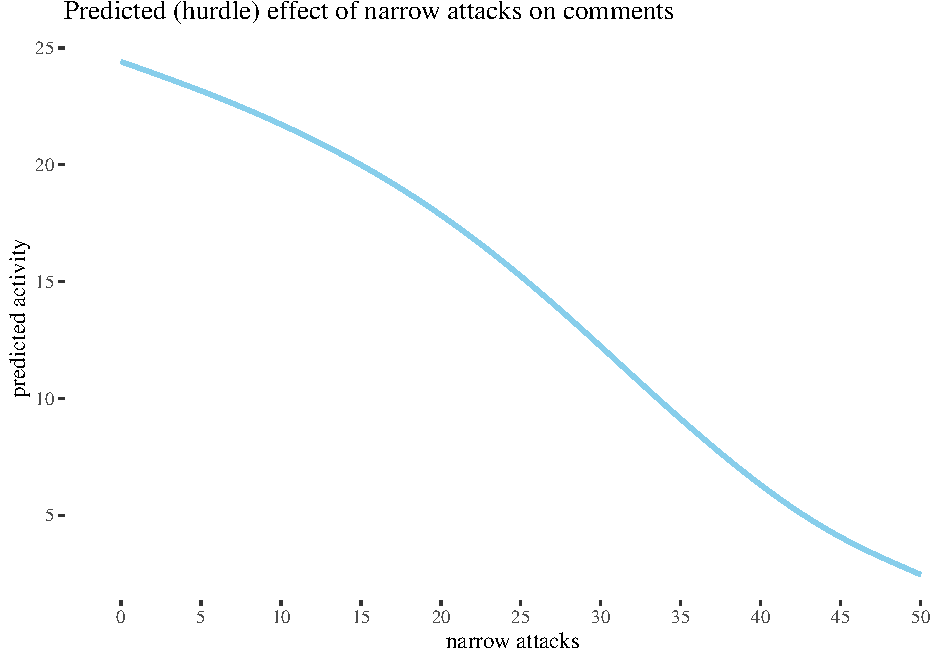
\includegraphics[width=1\linewidth]{redditAnalysisWalkthrough_files/figure-latex/unnamed-chunk-99-1} \end{center}
\end{subfigure}

\begin{subfigure}[b]{0.45\textwidth}

\begin{center}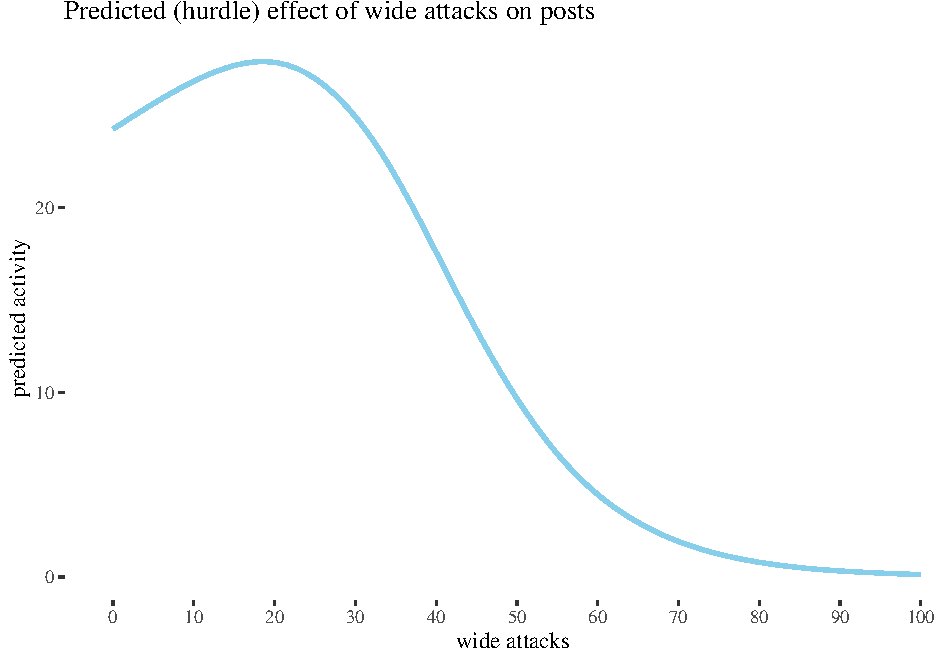
\includegraphics[width=1\linewidth]{redditAnalysisWalkthrough_files/figure-latex/unnamed-chunk-100-1} \end{center}
\end{subfigure}
\hfill
\begin{subfigure}[b]{0.45\textwidth}

\begin{center}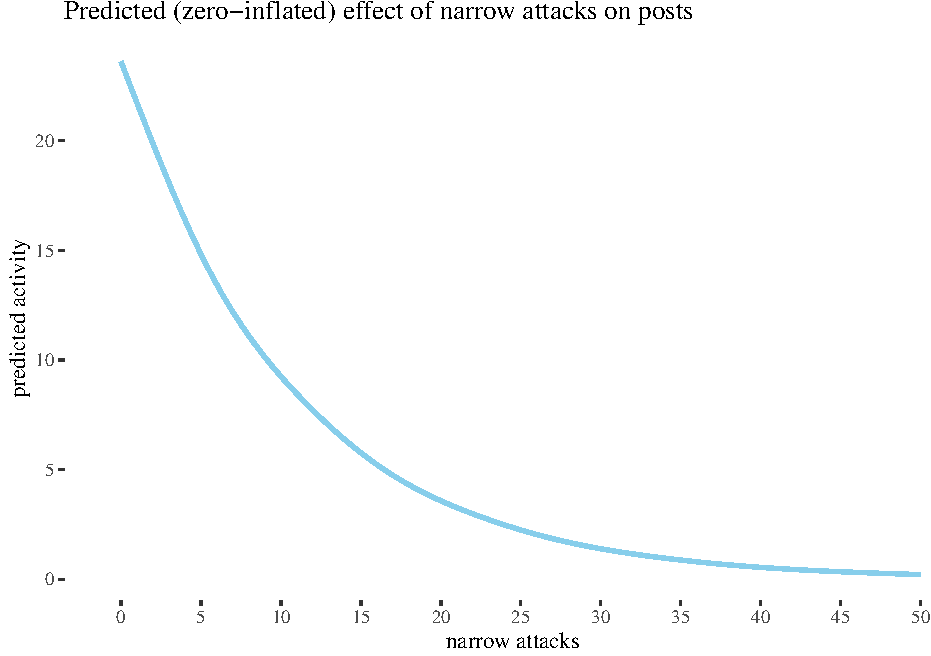
\includegraphics[width=1\linewidth]{redditAnalysisWalkthrough_files/figure-latex/unnamed-chunk-101-1} \end{center}
\end{subfigure}

\centering
\begin{subfigure}[t]{0.45\textwidth}

\begin{center}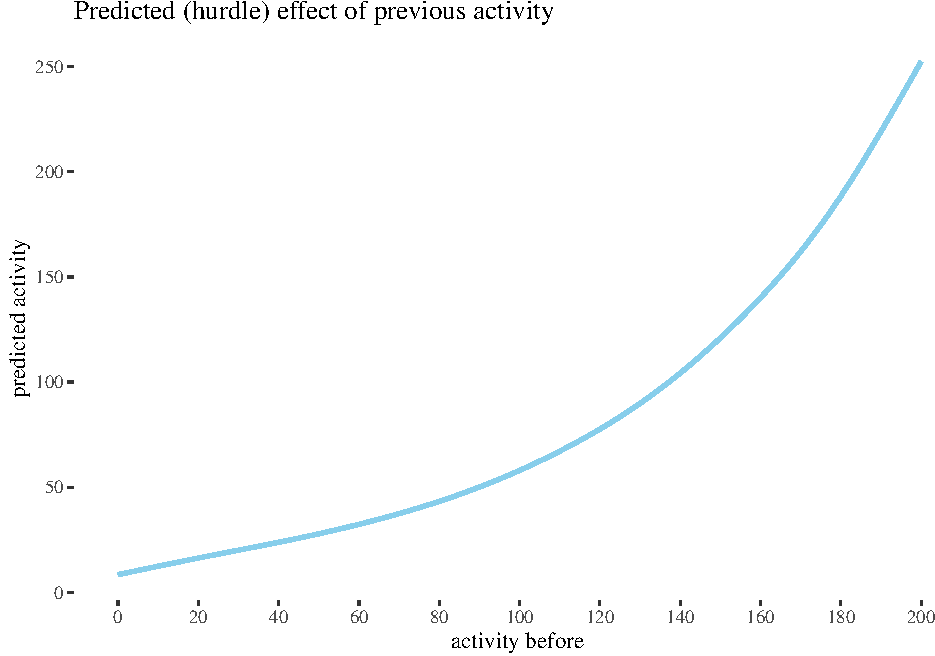
\includegraphics[width=1\linewidth]{redditAnalysisWalkthrough_files/figure-latex/unnamed-chunk-102-1} \end{center}
\end{subfigure}

\caption{Predicted effects of selected variables on activity with other variables fixed at their mean values, hurdle model.}
\label{fig:effects}
\end{figure}

Finally, to make sure our choice to use the hurdle model was not crucial
for these results, we also provide effect plots for the full
zero-inflated model.

\footnotesize

\begin{Shaded}
\begin{Highlighting}[]
\NormalTok{effSizePlotZ <-}\StringTok{ }\ControlFlowTok{function}\NormalTok{(columnno, }\DataTypeTok{range =} \DecValTok{40}\NormalTok{, }\DataTypeTok{by =} \DecValTok{5}\NormalTok{) \{}
\NormalTok{    EffDf <-}\StringTok{ }\NormalTok{baseEffDf}
\NormalTok{    EffDf[, columnno] <-}\StringTok{ }\DecValTok{0}\OperatorTok{:}\DecValTok{4000}
\NormalTok{    EffDf}\OperatorTok{$}\NormalTok{prediction <-}\StringTok{ }\KeywordTok{predict}\NormalTok{(ZNBfull, EffDf)}
    \KeywordTok{ggplot}\NormalTok{(EffDf, }\KeywordTok{aes}\NormalTok{(}\DataTypeTok{x =}\NormalTok{ EffDf[, columnno], }\DataTypeTok{y =}\NormalTok{ prediction)) }\OperatorTok{+}
\StringTok{        }\KeywordTok{geom_smooth}\NormalTok{(}\DataTypeTok{alpha =} \FloatTok{0.5}\NormalTok{, }\DataTypeTok{col =} \StringTok{"skyblue"}\NormalTok{, }\DataTypeTok{se =} \OtherTok{FALSE}\NormalTok{) }\OperatorTok{+}
\StringTok{        }\KeywordTok{scale_x_continuous}\NormalTok{(}\DataTypeTok{breaks =} \KeywordTok{seq}\NormalTok{(}\DecValTok{0}\NormalTok{, range, }\DataTypeTok{by =}\NormalTok{ by), }\DataTypeTok{limits =} \KeywordTok{c}\NormalTok{(}\OperatorTok{-}\DecValTok{1}\NormalTok{,}
\NormalTok{            range)) }\OperatorTok{+}\StringTok{ }\NormalTok{th }\OperatorTok{+}\StringTok{ }\KeywordTok{ylab}\NormalTok{(}\StringTok{"predicted activity"}\NormalTok{)}
\NormalTok{\}}

\NormalTok{effLOZ <-}\StringTok{ }\KeywordTok{effSizePlotZ}\NormalTok{(}\DecValTok{1}\NormalTok{, }\DecValTok{500}\NormalTok{, }\DecValTok{50}\NormalTok{)  }\CommentTok{#wide only}
\NormalTok{effHZ <-}\StringTok{ }\KeywordTok{effSizePlotZ}\NormalTok{(}\DecValTok{2}\NormalTok{, }\DecValTok{50}\NormalTok{, }\DecValTok{5}\NormalTok{)  }\CommentTok{#high on comments}
\NormalTok{effPlZ <-}\StringTok{ }\KeywordTok{effSizePlotZ}\NormalTok{(}\DecValTok{3}\NormalTok{, }\DecValTok{100}\NormalTok{, }\DecValTok{10}\NormalTok{)  }\CommentTok{#pl}
\NormalTok{effPhZ <-}\StringTok{ }\KeywordTok{effSizePlotZ}\NormalTok{(}\DecValTok{4}\NormalTok{, }\DecValTok{50}\NormalTok{, }\DecValTok{5}\NormalTok{)  }\CommentTok{#ph}
\NormalTok{effAZ <-}\StringTok{ }\KeywordTok{effSizePlotZ}\NormalTok{(}\DecValTok{5}\NormalTok{, }\DecValTok{200}\NormalTok{, }\DecValTok{20}\NormalTok{)  }\CommentTok{#abefore}
\end{Highlighting}
\end{Shaded}

\normalsize

\begin{figure}
\begin{subfigure}[b]{0.45\textwidth}

\begin{center}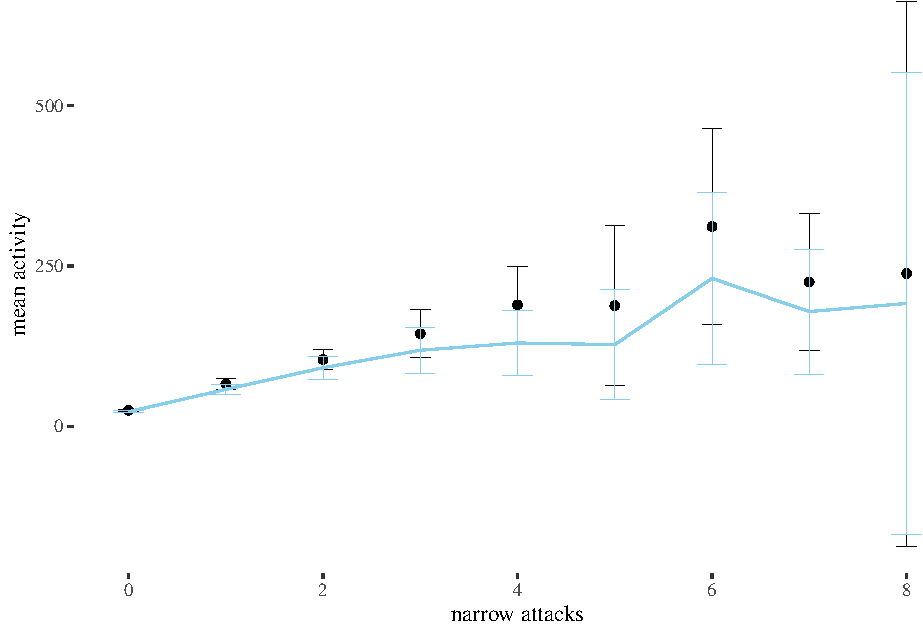
\includegraphics[width=1\linewidth]{redditAnalysisWalkthrough_files/figure-latex/unnamed-chunk-104-1} \end{center}
\end{subfigure}
\hfill
\begin{subfigure}[b]{0.45\textwidth}

\begin{center}\includegraphics[width=1\linewidth]{redditAnalysisWalkthrough_files/figure-latex/unnamed-chunk-105-1} \end{center}
\end{subfigure}

\begin{subfigure}[b]{0.45\textwidth}

\begin{center}\includegraphics[width=1\linewidth]{redditAnalysisWalkthrough_files/figure-latex/unnamed-chunk-106-1} \end{center}
\end{subfigure}
\hfill
\begin{subfigure}[b]{0.45\textwidth}

\begin{center}\includegraphics[width=1\linewidth]{redditAnalysisWalkthrough_files/figure-latex/unnamed-chunk-107-1} \end{center}
\end{subfigure}

\centering
\begin{subfigure}[t]{0.45\textwidth}

\begin{center}\includegraphics[width=1\linewidth]{redditAnalysisWalkthrough_files/figure-latex/unnamed-chunk-108-1} \end{center}
\end{subfigure}

\caption{Predicted effects of selected variables on activity with other variables fixed at their mean values, zero-inflated model.}
\label{fig:effects2}
\end{figure}

Another way to use this information is to inspect the table of activity
counts that the model expects based on the number of personal attacks on
a post received in the before period, assuming all the other input
variables are kept at their mean values:

\footnotesize

\begin{Shaded}
\begin{Highlighting}[]
\NormalTok{EffSumHighTable <-}\StringTok{ }\NormalTok{baseEffDf[}\DecValTok{0}\OperatorTok{:}\DecValTok{20}\NormalTok{, ]}
\NormalTok{EffSumHighTable[, }\DecValTok{4}\NormalTok{] <-}\StringTok{ }\DecValTok{0}\OperatorTok{:}\DecValTok{19}
\NormalTok{EffSumHighTable}\OperatorTok{$}\NormalTok{prediction <-}\StringTok{ }\KeywordTok{predict}\NormalTok{(HNBfull, EffSumHighTable)}
\NormalTok{EffTablePosts <-}\StringTok{ }\KeywordTok{rbind}\NormalTok{(EffSumHighTable}\OperatorTok{$}\NormalTok{sumPhBefore, }\KeywordTok{round}\NormalTok{(EffSumHighTable}\OperatorTok{$}\NormalTok{prediction))}
\KeywordTok{rownames}\NormalTok{(EffTablePosts) <-}\StringTok{ }\KeywordTok{c}\NormalTok{(}\StringTok{"attacks"}\NormalTok{, }\StringTok{"expected activity"}\NormalTok{)}
\KeywordTok{mykable}\NormalTok{(EffTablePosts) }\OperatorTok
\StringTok{    }\KeywordTok{kable_styling}\NormalTok{(}\DataTypeTok{latex_options =} \StringTok{"scale_down"}\NormalTok{)}
\end{Highlighting}
\end{Shaded}

\begin{table}
\centering\begingroup\fontsize{9}{11}\selectfont

\resizebox{\linewidth}{!}{
\begin{tabular}{lrrrrrrrrrrrrrrrrrrrr}
\toprule
\cellcolor{gray!6}{attacks} & \cellcolor{gray!6}{0} & \cellcolor{gray!6}{1} & \cellcolor{gray!6}{2} & \cellcolor{gray!6}{3} & \cellcolor{gray!6}{4} & \cellcolor{gray!6}{5} & \cellcolor{gray!6}{6} & \cellcolor{gray!6}{7} & \cellcolor{gray!6}{8} & \cellcolor{gray!6}{9} & \cellcolor{gray!6}{10} & \cellcolor{gray!6}{11} & \cellcolor{gray!6}{12} & \cellcolor{gray!6}{13} & \cellcolor{gray!6}{14} & \cellcolor{gray!6}{15} & \cellcolor{gray!6}{16} & \cellcolor{gray!6}{17} & \cellcolor{gray!6}{18} & \cellcolor{gray!6}{19}\\
expected activity & 24 & 22 & 19 & 17 & 15 & 13 & 11 & 10 & 9 & 8 & 7 & 6 & 6 & 5 & 5 & 4 & 4 & 3 & 3 & 3\\
\bottomrule
\end{tabular}}
\endgroup{}
\end{table}

\normalsize

The predictions are similar, except for the predicted results of wide
only attacks on posts. This perhaps can be explained by observing that
such cases of personal attacks sometimes represent situations in which
the users actually agree with the original post (see our remark in the
beginning of the section about data gathering and selection), and in
some cases the attacks are critical of the author, so there is much more
variation in this group and precise modeling is harder.

It should be kept in mind that the model is built on up to 27 attacks in
the \textsf{before} period, with really low number of attacks above 8,
so the prediction here is an extrapolation, not an interpolation.
Further studies for longer periods are needed to get a more reliable
estimate allowing for interpolation in this respect.

One might have reasoned about our previous analyses as follows: attacks
in the before period correlate with activity before, and it is activity
before that is the real predictor of activity after. This could be
supported by observing that the \(p\)-value for the hurdle model is
really low for activity before. Pearson correlation coefficient for
narrow attacks before and activity before is \(r(3671)\approx\) 0.437
and \(r(3671)\approx\) 0.332 for activity after. However, activity
before is a much better correlate of activity after, \(r(3671)\approx\)
0.845 --- all correlations with \(p\)-value \(<2.2e-16\), and regression
analysis (inspect the effect plots) indicates that activity before and
high attacks before actually go in the opposite directions.

\section{Regression to the mean?}

Another problem plaguing observational studies is
\textbf{regression to the mean}. If the probability of any particular
message being attacked is fairly low, users who have received an attack
are quite likely to have posted more content than the treatment group,
and perhaps those who posted more content in the \textsf{before} period
are more likely to post less in the \textsf{after} period. This concern
might be elevated by the observation that activity before indeed
increases with the number of attacks received and that the activity drop
increases with \textsf{activity} before.

\footnotesize

\begin{Shaded}
\begin{Highlighting}[]
\NormalTok{attacksb <-}\StringTok{ }\DecValTok{0}\OperatorTok{:}\DecValTok{8}
\NormalTok{maxb <-}\StringTok{ }\KeywordTok{max}\NormalTok{(attacks)}
\NormalTok{lowb <-}\StringTok{ }\KeywordTok{numeric}\NormalTok{(max }\OperatorTok{+}\StringTok{ }\DecValTok{1}\NormalTok{)}
\NormalTok{highb <-}\StringTok{ }\KeywordTok{numeric}\NormalTok{(max }\OperatorTok{+}\StringTok{ }\DecValTok{1}\NormalTok{)}
\NormalTok{mb <-}\StringTok{ }\KeywordTok{numeric}\NormalTok{(max }\OperatorTok{+}\StringTok{ }\DecValTok{1}\NormalTok{)}
\NormalTok{pb <-}\StringTok{ }\KeywordTok{numeric}\NormalTok{(max }\OperatorTok{+}\StringTok{ }\DecValTok{1}\NormalTok{)}
\NormalTok{tb <-}\StringTok{ }\KeywordTok{list}\NormalTok{()}

\ControlFlowTok{for}\NormalTok{ (attacks }\ControlFlowTok{in}\NormalTok{ attacksb) \{}
\NormalTok{    t[[attacks }\OperatorTok{+}\StringTok{ }\DecValTok{1}\NormalTok{]] <-}\StringTok{ }\KeywordTok{t.test}\NormalTok{(data[data}\OperatorTok{$}\NormalTok{sumHighBefore }\OperatorTok{==}\StringTok{ }\NormalTok{attacks,}
\NormalTok{        ]}\OperatorTok{$}\NormalTok{activityBefore)}

\NormalTok{    lowb[attacks }\OperatorTok{+}\StringTok{ }\DecValTok{1}\NormalTok{] <-}\StringTok{ }\NormalTok{t[[attacks }\OperatorTok{+}\StringTok{ }\DecValTok{1}\NormalTok{]]}\OperatorTok{$}\NormalTok{conf.int[}\DecValTok{1}\NormalTok{]}
\NormalTok{    highb[attacks }\OperatorTok{+}\StringTok{ }\DecValTok{1}\NormalTok{] <-}\StringTok{ }\NormalTok{t[[attacks }\OperatorTok{+}\StringTok{ }\DecValTok{1}\NormalTok{]]}\OperatorTok{$}\NormalTok{conf.int[}\DecValTok{2}\NormalTok{]}
\NormalTok{    mb[attacks }\OperatorTok{+}\StringTok{ }\DecValTok{1}\NormalTok{] <-}\StringTok{ }\NormalTok{t[[attacks }\OperatorTok{+}\StringTok{ }\DecValTok{1}\NormalTok{]]}\OperatorTok{$}\NormalTok{estimate}
\NormalTok{    pb[attacks }\OperatorTok{+}\StringTok{ }\DecValTok{1}\NormalTok{] <-}\StringTok{ }\NormalTok{t[[attacks }\OperatorTok{+}\StringTok{ }\DecValTok{1}\NormalTok{]]}\OperatorTok{$}\NormalTok{p.value}
\NormalTok{\}}
\NormalTok{highTableb <-}\StringTok{ }\KeywordTok{as.data.frame}\NormalTok{(}\KeywordTok{round}\NormalTok{(}\KeywordTok{rbind}\NormalTok{(}\DecValTok{0}\OperatorTok{:}\DecValTok{8}\NormalTok{, lowb, mb, highb,}
\NormalTok{    pb), }\DecValTok{3}\NormalTok{))}
\KeywordTok{rownames}\NormalTok{(highTableb) <-}\StringTok{ }\KeywordTok{c}\NormalTok{(}\StringTok{"attacks"}\NormalTok{, }\StringTok{"CIlow"}\NormalTok{, }\StringTok{"estimatedm"}\NormalTok{, }\StringTok{"CIhigh"}\NormalTok{,}
    \StringTok{"p-value"}\NormalTok{)}

\NormalTok{before <-}\StringTok{ }\KeywordTok{as.data.frame}\NormalTok{(}\KeywordTok{t}\NormalTok{(highTableb))}

\NormalTok{attacksa <-}\StringTok{ }\DecValTok{0}\OperatorTok{:}\DecValTok{8}
\NormalTok{maxa <-}\StringTok{ }\KeywordTok{max}\NormalTok{(attacksa)}
\NormalTok{lowa <-}\StringTok{ }\KeywordTok{numeric}\NormalTok{(max }\OperatorTok{+}\StringTok{ }\DecValTok{1}\NormalTok{)}
\NormalTok{higha <-}\StringTok{ }\KeywordTok{numeric}\NormalTok{(max }\OperatorTok{+}\StringTok{ }\DecValTok{1}\NormalTok{)}
\NormalTok{ma <-}\StringTok{ }\KeywordTok{numeric}\NormalTok{(max }\OperatorTok{+}\StringTok{ }\DecValTok{1}\NormalTok{)}
\NormalTok{pa <-}\StringTok{ }\KeywordTok{numeric}\NormalTok{(max }\OperatorTok{+}\StringTok{ }\DecValTok{1}\NormalTok{)}
\NormalTok{ta <-}\StringTok{ }\KeywordTok{list}\NormalTok{()}
\ControlFlowTok{for}\NormalTok{ (attacks }\ControlFlowTok{in}\NormalTok{ attacksa) \{}
\NormalTok{    ta[[attacks }\OperatorTok{+}\StringTok{ }\DecValTok{1}\NormalTok{]] <-}\StringTok{ }\KeywordTok{t.test}\NormalTok{(data[data}\OperatorTok{$}\NormalTok{sumHighBefore }\OperatorTok{==}\StringTok{ }\NormalTok{attacks,}
\NormalTok{        ]}\OperatorTok{$}\NormalTok{activityAfter)}
\NormalTok{    lowa[attacks }\OperatorTok{+}\StringTok{ }\DecValTok{1}\NormalTok{] <-}\StringTok{ }\NormalTok{ta[[attacks }\OperatorTok{+}\StringTok{ }\DecValTok{1}\NormalTok{]]}\OperatorTok{$}\NormalTok{conf.int[}\DecValTok{1}\NormalTok{]}
\NormalTok{    higha[attacks }\OperatorTok{+}\StringTok{ }\DecValTok{1}\NormalTok{] <-}\StringTok{ }\NormalTok{ta[[attacks }\OperatorTok{+}\StringTok{ }\DecValTok{1}\NormalTok{]]}\OperatorTok{$}\NormalTok{conf.int[}\DecValTok{2}\NormalTok{]}
\NormalTok{    ma[attacks }\OperatorTok{+}\StringTok{ }\DecValTok{1}\NormalTok{] <-}\StringTok{ }\NormalTok{ta[[attacks }\OperatorTok{+}\StringTok{ }\DecValTok{1}\NormalTok{]]}\OperatorTok{$}\NormalTok{estimate}
\NormalTok{    pa[attacks }\OperatorTok{+}\StringTok{ }\DecValTok{1}\NormalTok{] <-}\StringTok{ }\NormalTok{ta[[attacks }\OperatorTok{+}\StringTok{ }\DecValTok{1}\NormalTok{]]}\OperatorTok{$}\NormalTok{p.value}
\NormalTok{\}}
\NormalTok{highTablea <-}\StringTok{ }\KeywordTok{as.data.frame}\NormalTok{(}\KeywordTok{round}\NormalTok{(}\KeywordTok{rbind}\NormalTok{(}\DecValTok{0}\OperatorTok{:}\DecValTok{8}\NormalTok{, lowa, ma, higha,}
\NormalTok{    pa), }\DecValTok{3}\NormalTok{))}
\KeywordTok{rownames}\NormalTok{(highTablea) <-}\StringTok{ }\KeywordTok{c}\NormalTok{(}\StringTok{"attacks"}\NormalTok{, }\StringTok{"CIlow"}\NormalTok{, }\StringTok{"estimatedm"}\NormalTok{, }\StringTok{"CIhigh"}\NormalTok{,}
    \StringTok{"p-value"}\NormalTok{)}
\NormalTok{after <-}\StringTok{ }\KeywordTok{as.data.frame}\NormalTok{(}\KeywordTok{t}\NormalTok{(highTablea))}

\KeywordTok{ggplot}\NormalTok{(before, }\KeywordTok{aes}\NormalTok{(}\DataTypeTok{x =}\NormalTok{ attacks, }\DataTypeTok{y =}\NormalTok{ estimatedm)) }\OperatorTok{+}\StringTok{ }\KeywordTok{geom_point}\NormalTok{() }\OperatorTok{+}
\StringTok{    }\KeywordTok{geom_errorbar}\NormalTok{(}\KeywordTok{aes}\NormalTok{(}\DataTypeTok{ymin =}\NormalTok{ CIlow, }\DataTypeTok{ymax =}\NormalTok{ CIhigh), }\DataTypeTok{width =} \FloatTok{0.2}\NormalTok{,}
        \DataTypeTok{size =} \FloatTok{0.2}\NormalTok{, }\DataTypeTok{position =} \KeywordTok{position_dodge}\NormalTok{(}\FloatTok{0.05}\NormalTok{)) }\OperatorTok{+}\StringTok{ }\NormalTok{th }\OperatorTok{+}\StringTok{ }\KeywordTok{xlab}\NormalTok{(}\StringTok{"narrow attacks"}\NormalTok{) }\OperatorTok{+}
\StringTok{    }\KeywordTok{ylab}\NormalTok{(}\StringTok{"mean activity"}\NormalTok{) }\OperatorTok{+}\StringTok{ }\KeywordTok{geom_line}\NormalTok{(}\DataTypeTok{data =}\NormalTok{ after, }\KeywordTok{aes}\NormalTok{(}\DataTypeTok{x =}\NormalTok{ attacks,}
    \DataTypeTok{y =}\NormalTok{ estimatedm), }\DataTypeTok{color =} \StringTok{"skyblue"}\NormalTok{) }\OperatorTok{+}\StringTok{ }\KeywordTok{geom_errorbar}\NormalTok{(}\DataTypeTok{data =}\NormalTok{ after,}
    \KeywordTok{aes}\NormalTok{(}\DataTypeTok{ymin =}\NormalTok{ CIlow, }\DataTypeTok{ymax =}\NormalTok{ CIhigh), }\DataTypeTok{width =} \FloatTok{0.3}\NormalTok{, }\DataTypeTok{size =} \FloatTok{0.2}\NormalTok{,}
    \DataTypeTok{color =} \StringTok{"skyblue"}\NormalTok{, }\DataTypeTok{position =} \KeywordTok{position_dodge}\NormalTok{(}\FloatTok{0.05}\NormalTok{))}
\end{Highlighting}
\end{Shaded}

\normalsize

\begin{figure}

\begin{center}\includegraphics[width=1\linewidth]{redditAnalysisWalkthrough_files/figure-latex/unnamed-chunk-111-1} \end{center}
\caption{Mean activity before (black) with 95\% CI error bars and after (blue) , grouped by the number of narrow attacks.}
\end{figure}

We visually inspect in Figure \ref{fig:regression} the relation between
the distance from the sample mean for \textsf{activityBefore} and the
activity change between week 1 and week 2, grouped by the number of
attacks received (for the cases for which we obtained significant
results in the classical analysis).

\footnotesize

\begin{Shaded}
\begin{Highlighting}[]
\NormalTok{h0 <-}\StringTok{ }\NormalTok{data[data}\OperatorTok{$}\NormalTok{sumHighBefore }\OperatorTok{==}\StringTok{ }\DecValTok{0}\NormalTok{, ]}
\NormalTok{h1 <-}\StringTok{ }\NormalTok{data[data}\OperatorTok{$}\NormalTok{sumHighBefore }\OperatorTok{==}\StringTok{ }\DecValTok{1}\NormalTok{, ]}
\NormalTok{h2 <-}\StringTok{ }\NormalTok{data[data}\OperatorTok{$}\NormalTok{sumHighBefore }\OperatorTok{==}\StringTok{ }\DecValTok{2}\NormalTok{, ]}
\NormalTok{h3 <-}\StringTok{ }\NormalTok{data[data}\OperatorTok{$}\NormalTok{sumHighBefore }\OperatorTok{==}\StringTok{ }\DecValTok{3}\NormalTok{, ]}
\NormalTok{h4 <-}\StringTok{ }\NormalTok{data[data}\OperatorTok{$}\NormalTok{sumHighBefore }\OperatorTok{==}\StringTok{ }\DecValTok{4}\NormalTok{, ]}

\NormalTok{distance <-}\StringTok{ }\ControlFlowTok{function}\NormalTok{(x) \{}
\NormalTok{    x }\OperatorTok{-}\StringTok{ }\KeywordTok{mean}\NormalTok{(data}\OperatorTok{$}\NormalTok{sumHighBefore)}
\NormalTok{\}}

\KeywordTok{library}\NormalTok{(gridExtra)}
\KeywordTok{grid.arrange}\NormalTok{(}\KeywordTok{ggplot}\NormalTok{(h0, }\KeywordTok{aes}\NormalTok{(}\DataTypeTok{x =} \KeywordTok{distance}\NormalTok{(activityBefore), }\DataTypeTok{y =}\NormalTok{ activityDiff)) }\OperatorTok{+}
\StringTok{    }\KeywordTok{geom_point}\NormalTok{(}\DataTypeTok{alpha =} \FloatTok{0.3}\NormalTok{, }\DataTypeTok{size =} \DecValTok{1}\NormalTok{, }\DataTypeTok{position =} \StringTok{"jitter"}\NormalTok{) }\OperatorTok{+}
\StringTok{    }\KeywordTok{geom_smooth}\NormalTok{(}\DataTypeTok{size =} \FloatTok{0.5}\NormalTok{, }\DataTypeTok{alpha =} \FloatTok{0.5}\NormalTok{) }\OperatorTok{+}\StringTok{ }\NormalTok{th }\OperatorTok{+}\StringTok{ }\KeywordTok{xlab}\NormalTok{(}\StringTok{"distance from sample mean"}\NormalTok{) }\OperatorTok{+}
\StringTok{    }\KeywordTok{ggtitle}\NormalTok{(}\StringTok{"0 narrow attacks"}\NormalTok{) }\OperatorTok{+}\StringTok{ }\KeywordTok{ylab}\NormalTok{(}\StringTok{"activity change"}\NormalTok{), }\KeywordTok{ggplot}\NormalTok{(h2,}
    \KeywordTok{aes}\NormalTok{(}\DataTypeTok{x =} \KeywordTok{distance}\NormalTok{(activityBefore), }\DataTypeTok{y =}\NormalTok{ activityDiff)) }\OperatorTok{+}\StringTok{ }\KeywordTok{geom_point}\NormalTok{(}\DataTypeTok{alpha =} \FloatTok{0.3}\NormalTok{,}
    \DataTypeTok{size =} \DecValTok{1}\NormalTok{, }\DataTypeTok{position =} \StringTok{"jitter"}\NormalTok{) }\OperatorTok{+}\StringTok{ }\KeywordTok{geom_smooth}\NormalTok{(}\DataTypeTok{size =} \FloatTok{0.5}\NormalTok{,}
    \DataTypeTok{alpha =} \FloatTok{0.5}\NormalTok{) }\OperatorTok{+}\StringTok{ }\NormalTok{th }\OperatorTok{+}\StringTok{ }\KeywordTok{xlab}\NormalTok{(}\StringTok{"distance from sample mean"}\NormalTok{) }\OperatorTok{+}\StringTok{ }\KeywordTok{ggtitle}\NormalTok{(}\StringTok{"2 narrow attacks"}\NormalTok{) }\OperatorTok{+}
\StringTok{    }\KeywordTok{ylab}\NormalTok{(}\StringTok{"activity change"}\NormalTok{), }\KeywordTok{ggplot}\NormalTok{(h3, }\KeywordTok{aes}\NormalTok{(}\DataTypeTok{x =} \KeywordTok{distance}\NormalTok{(activityBefore),}
    \DataTypeTok{y =}\NormalTok{ activityDiff)) }\OperatorTok{+}\StringTok{ }\KeywordTok{geom_point}\NormalTok{(}\DataTypeTok{alpha =} \FloatTok{0.3}\NormalTok{, }\DataTypeTok{size =} \DecValTok{1}\NormalTok{, }\DataTypeTok{position =} \StringTok{"jitter"}\NormalTok{) }\OperatorTok{+}
\StringTok{    }\KeywordTok{geom_smooth}\NormalTok{(}\DataTypeTok{size =} \FloatTok{0.5}\NormalTok{, }\DataTypeTok{alpha =} \FloatTok{0.5}\NormalTok{) }\OperatorTok{+}\StringTok{ }\NormalTok{th }\OperatorTok{+}\StringTok{ }\KeywordTok{xlab}\NormalTok{(}\StringTok{"distance from sample mean"}\NormalTok{) }\OperatorTok{+}
\StringTok{    }\KeywordTok{ggtitle}\NormalTok{(}\StringTok{"3 narrow attacks"}\NormalTok{) }\OperatorTok{+}\StringTok{ }\KeywordTok{ylab}\NormalTok{(}\StringTok{"activity change"}\NormalTok{), }\KeywordTok{ggplot}\NormalTok{(h4,}
    \KeywordTok{aes}\NormalTok{(}\DataTypeTok{x =} \KeywordTok{distance}\NormalTok{(activityBefore), }\DataTypeTok{y =}\NormalTok{ activityDiff)) }\OperatorTok{+}\StringTok{ }\KeywordTok{geom_point}\NormalTok{(}\DataTypeTok{alpha =} \FloatTok{0.3}\NormalTok{,}
    \DataTypeTok{size =} \DecValTok{1}\NormalTok{, }\DataTypeTok{position =} \StringTok{"jitter"}\NormalTok{) }\OperatorTok{+}\StringTok{ }\KeywordTok{geom_smooth}\NormalTok{(}\DataTypeTok{size =} \FloatTok{0.5}\NormalTok{,}
    \DataTypeTok{alpha =} \FloatTok{0.5}\NormalTok{) }\OperatorTok{+}\StringTok{ }\NormalTok{th }\OperatorTok{+}\StringTok{ }\KeywordTok{xlab}\NormalTok{(}\StringTok{"distance from sample mean"}\NormalTok{) }\OperatorTok{+}\StringTok{ }\KeywordTok{ggtitle}\NormalTok{(}\StringTok{"4 narrow attacks"}\NormalTok{) }\OperatorTok{+}
\StringTok{    }\KeywordTok{ylab}\NormalTok{(}\StringTok{"activity change"}\NormalTok{))}
\end{Highlighting}
\end{Shaded}

\normalsize

\begin{figure}

\begin{center}\includegraphics[width=1\linewidth]{redditAnalysisWalkthrough_files/figure-latex/unnamed-chunk-113-1} \end{center}
\caption{Distance from sample mean vs. activity change, grouped by the number of attacks (plot for 1 narrow attack omitted, as it is visually not very too distinct from the one for 0 attacks).}
\label{fig:regression}
\end{figure}

First, in an inspection of the control group, the smoothing might
suggest some correlation between the distance from the mean and the
activity drop. However, the sharp cut-off at the bottom is there because
one cannot drop their activity below the previous activity level. So
users closer to the mean didn't even have the lower options available,
and this restriction might be partially responsible for the smoothing
line going downwards. Moreover, Spearman correlation between the
distance from the mean and the activity change is -0.269, which is
fairly weak. Pearson's \(\rho\) is not very different ( -0.255), but we
need to be careful here, because the relation doesn't seem very linear
(\(p\)-values for correlation tests are both \(<0.001\)). If, however,
we follow this line of reasoning, the distance from the mean would
explain only \(R^2 =\) 0.065 of the variability in the activity change
in the control group.

The impression of regression to the mean disappears when we look at
\textsf{activityScore}, that is, activity change in proportion to
previous activity (Fig. \ref{fig:regression2}).

\begin{figure}

\begin{center}\includegraphics[width=1\linewidth]{redditAnalysisWalkthrough_files/figure-latex/unnamed-chunk-114-1} \end{center}
\caption{Distance from sample mean vs. activity score, grouped by the number of attacks (plot for 1 narrow attack omitted, as it is visually not too distinct from the one for 0 attacks).}
\label{fig:regression2}
\end{figure}

Plots for \(>0\) attacks with gam smoothing does not suggest regression
to the mean: it is not the case that attacked users with higher activity
before indeed tend to have lower activity in the second week.

Next, notice that restricting the dataset to users with similar activity
before still results in uneven activity change between the groups. We
focus focus on users with \textsf{activityBefore} restricted to the
third quartile of the whole sample (44), narrow attacks in \$\{0,1,2,3,
4\} and estimate their \textsf{activityScore} proportional drop.

\footnotesize

\begin{Shaded}
\begin{Highlighting}[]
\NormalTok{iqr0 <-}\StringTok{ }\NormalTok{data[data}\OperatorTok{$}\NormalTok{sumHighBefore }\OperatorTok{==}\StringTok{ }\DecValTok{0} \OperatorTok{&}\StringTok{ }\NormalTok{data}\OperatorTok{$}\NormalTok{activityBefore }\OperatorTok{<=}
\StringTok{    }\DecValTok{44}\NormalTok{, ]}
\NormalTok{iqr1 <-}\StringTok{ }\NormalTok{data[data}\OperatorTok{$}\NormalTok{sumHighBefore }\OperatorTok{==}\StringTok{ }\DecValTok{1} \OperatorTok{&}\StringTok{ }\NormalTok{data}\OperatorTok{$}\NormalTok{activityBefore }\OperatorTok{<=}
\StringTok{    }\DecValTok{44}\NormalTok{, ]}
\NormalTok{iqr2 <-}\StringTok{ }\NormalTok{data[data}\OperatorTok{$}\NormalTok{sumHighBefore }\OperatorTok{==}\StringTok{ }\DecValTok{2} \OperatorTok{&}\StringTok{ }\NormalTok{data}\OperatorTok{$}\NormalTok{activityBefore }\OperatorTok{<=}
\StringTok{    }\DecValTok{44}\NormalTok{, ]}
\NormalTok{iqr3 <-}\StringTok{ }\NormalTok{data[data}\OperatorTok{$}\NormalTok{sumHighBefore }\OperatorTok{==}\StringTok{ }\DecValTok{3} \OperatorTok{&}\StringTok{ }\NormalTok{data}\OperatorTok{$}\NormalTok{activityBefore }\OperatorTok{<=}
\StringTok{    }\DecValTok{44}\NormalTok{, ]}
\NormalTok{iqr4 <-}\StringTok{ }\NormalTok{data[data}\OperatorTok{$}\NormalTok{sumHighBefore }\OperatorTok{==}\StringTok{ }\DecValTok{4} \OperatorTok{&}\StringTok{ }\NormalTok{data}\OperatorTok{$}\NormalTok{activityBefore }\OperatorTok{<=}
\StringTok{    }\DecValTok{44}\NormalTok{, ]}

\KeywordTok{t.test}\NormalTok{(iqr0}\OperatorTok{$}\NormalTok{activityScore)}
\KeywordTok{t.test}\NormalTok{(iqr1}\OperatorTok{$}\NormalTok{activityScore)}
\KeywordTok{t.test}\NormalTok{(iqr2}\OperatorTok{$}\NormalTok{activityScore)}
\KeywordTok{t.test}\NormalTok{(iqr3}\OperatorTok{$}\NormalTok{activityScore)}
\KeywordTok{t.test}\NormalTok{(iqr4}\OperatorTok{$}\NormalTok{activityScore)}
\end{Highlighting}
\end{Shaded}

\normalsize  The estimated means of proportional changes are
\(0.05, 0.11, -0.09,-0.35, -0.7\) with decreasing p-values falling below
.05 at the number of attacks \(=3, 4\) and \(p\)-value 0.002 for four
attacks (that is, 0.01 with Bonferroni correction for multiple testing),
despite the group sizes for three and four attacks being fairly low (49
for two, 13 for three, 7 for four). By the way, note that with this
activity restriction, receiving one attack does not seem to have much
impact on user's activity.

Further, to adjust for regression to the mean, it is sometimes
recommended to use ANCOVA to correct for prior differences in pretest
measurements. In our case, a statistically significant difference for
different number of attacks received remains after correcting for
differences in activity before.

\footnotesize

\begin{Shaded}
\begin{Highlighting}[]
\KeywordTok{library}\NormalTok{(rstatix)}
\NormalTok{data}\OperatorTok{$}\NormalTok{fhigh <-}\StringTok{ }\KeywordTok{as.factor}\NormalTok{(data}\OperatorTok{$}\NormalTok{sumHighBefore)}
\NormalTok{data }\OperatorTok
\StringTok{    }\KeywordTok{anova_test}\NormalTok{(activityDiff }\OperatorTok{~}\StringTok{ }\NormalTok{activityBefore }\OperatorTok{+}\StringTok{ }\NormalTok{fhigh)}
\end{Highlighting}
\end{Shaded}

\normalsize

\begin{table}
\footnotesize

\begin{tabular}{l|r|r|r|r|l|r}
\hline
Effect & DFn & DFd & F & p & p<.05 & ges\\
\hline
activityBefore & 1 & 3651 & 577.220 & 0 & * & 0.137\\
\hline
fhigh & 20 & 3651 & 10.214 & 0 & * & 0.053\\
\hline
\end{tabular}
\normalsize 
\caption{Results of ANCOVA test of activity difference vs. activity before and the number of narrow attacks received.}
\end{table}

Finally, the model-theoretic analysis already corrects for activity
before, and estimates the effect size of the other variables keeping
activity before fixed at the mean level. So, regression to the mean,
while it might play a small part, does not seem to explain the
differences. However, the potential effects of regression to the mean
have to be kept in mind in future observational studies and replication
attempts.

\newpage

\section*{References}

\hypertarget{refs}{}
\hypertarget{ref-Akaike1974model}{}
Akaike, H. (1974). A new look at the statistical model identification.
\emph{IEEE Transactions on Automatic Control}, \emph{19}(6), 716--723.

\hypertarget{ref-Kruschke2015}{}
Kruschke, J. (2015). \emph{Doing Bayesian data analysis; a tutorial with
R, JAGS, and Stan}.

\hypertarget{ref-ptaszynski2018cyberbullying}{}
Ptaszyński, M., Leliwa, G., Piech, M., \& Smywiński-Pohl, A. (2018).
Cyberbullying detection--technical report 2/2018, Department of Computer
Science AGH, University of Science and Technology. \emph{arXiv preprint
arXiv:1808.00926}.

\hypertarget{ref-Tukey1949}{}
Tukey, J. W. (1949). Comparing individual means in the analysis of
variance. \emph{Biometrics}, \emph{5}(2), 99. JSTOR. Retrieved from
\url{https://doi.org/10.2307/3001913}

\hypertarget{ref-valkenburg2006friend}{}
Valkenburg, P. M., Peter, J., \& Schouten, A. P. (2006). Friend
networking sites and their relationship to adolescents' well-being and
social self-esteem. \emph{CyberPsychology \& behavior}, \emph{9}(5),
584--590. Mary Ann Liebert, Inc. 2 Madison Avenue Larchmont, NY 10538
USA.

\hypertarget{ref-wise2006moderation}{}
Wise, K., Hamman, B., \& Thorson, K. (2006). Moderation, response rate,
and message interactivity: Features of online communities and their
effects on intent to participate. \emph{Journal of Computer-Mediated
Communication}, \emph{12}(1), 24--41. Oxford University Press Oxford,
UK.

\hypertarget{ref-wroczynski2019system}{}
Wroczynski, M., \& Leliwa, G. (2019, sep\textasciitilde{}5). System and
method for detecting undesirable and potentially harmful online
behavior. Google Patents.

\hypertarget{ref-zong2019social}{}
Zong, W., Yang, J., \& Bao, Z. (2019). Social network fatigue affecting
continuance intention of social networking services. \emph{Data
Technologies and Applications}. Emerald Publishing Limited.

\end{document}
